\part{Introduction}
\label{introduction}

\chapter{Sociocracy 3.0{\ldots}}
\label{sociocracy3.0...}

{\ldots}is a method for growing \textbf{effective, agile and resilient organization}s of \textbf{any size,} from small start-ups to large international networks and nationwide, multi-agency collaboration.

{\ldots}provides a collection of \textbf{principles and patterns} to \textbf{dynamically steer and evolve organizations}.

{\ldots}incrementally processes \textbf{available information} into \textbf{continuous improvement of products, processes and skills}.

{\ldots}helps organizations making \textbf{the best use of the talent already present}, and to grow flexible organizational \textbf{structures that support effective travel of information}.

{\ldots}contains a \textbf{soft, iterative approach to implementation} that \textbf{meets organizations where they} are and helps them move forward at their own pace.

{\ldots}draws on the \emph{collective intelligence} of the group

{\ldots}facilitates the development of strategies that are “\emph{good enough for now}” and “\emph{safe enough to try}”

{\ldots}fosters accountability and a sense of engagement
{\ldots}is a transformational mechanism for both individuals and the whole organization

Sociocracy 3.0 may be applied within{\ldots}

\begin{itemize}
\item {\ldots}startups

\item {\ldots}small and medium businesses

\item {\ldots}large international, networked organizations

\item {\ldots}families

\item {\ldots}investor-funded organizations

\item {\ldots}communities

\end{itemize}

\textbf{What’s in a word?}

\begin{itemize}
\item \emph{socio}

\begin{itemize}
\item from Latin \emph{socius} - companion, friend

\end{itemize}

\item \emph{-cracy}

\begin{itemize}
\item from Ancient Greek krátos - “power, rule”

\end{itemize}

\item different to the rule of the \emph{demos}

\begin{itemize}
\item the general mass of people with voting privileges

\end{itemize}

\end{itemize}

\chapter{A Brief History of Sociocracy From 1851 to Today}
\label{abriefhistoryofsociocracyfrom1851totoday}

\begin{figure}[htbp]
\centering
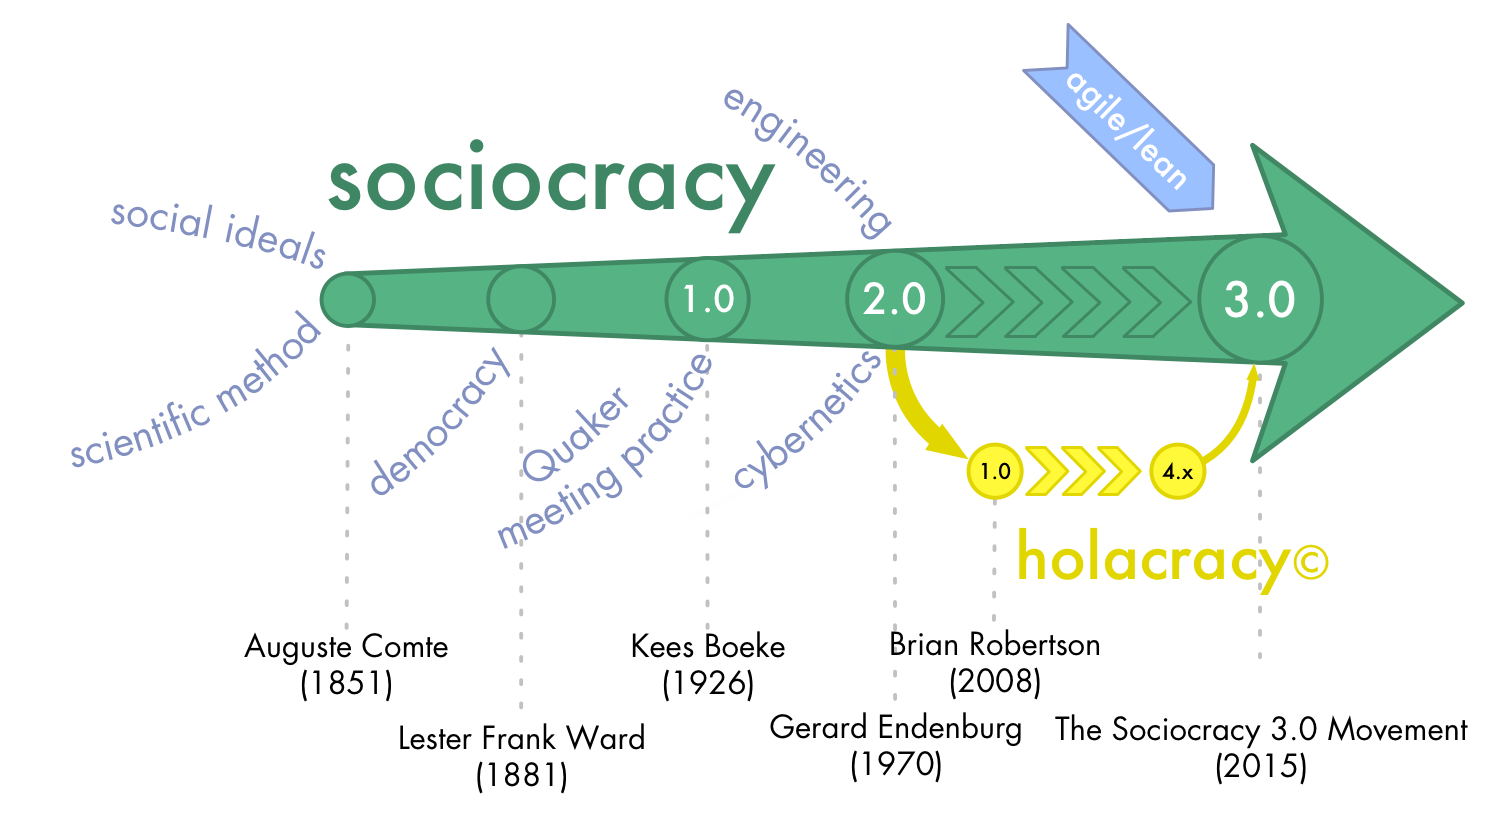
\includegraphics[keepaspectratio,width=\textwidth,height=0.75\textheight]{img/general/history.png}
\end{figure}

\begin{itemize}
\item 1851 – Auguste Comte

\begin{itemize}
\item Scientific method applied to society

\item Sociocracy is “\emph{the social order of the future}” - not yet achievable but inevitable

\end{itemize}

\item 1881 – Lester Frank Ward

\begin{itemize}
\item redefined the term Sociocracy to describe the rule of the people with relationships with each other

\end{itemize}

\item 1926 --1954 - Kees Boeke

\begin{itemize}
\item Established the first sociocracy in his residential school (based on Quaker consensus principles)

\item Book “\emph{Sociocracy: Democracy as it might be}” (1945)

\end{itemize}

\item 1970's - Gerard Endenburg

\begin{itemize}
\item Student in Kees Boeke’s school

\item Integrated principles from Engineering and Cybernetics

\item In his company Endenburg Electrotechniek he evolved “\emph{The Sociocratic Circle-Organization Method}” (later becoming ``\emph{The Sociocratic Method}'')

\end{itemize}

\item 1978 - Sociocratisch Centrum Utrecht

\begin{itemize}
\item created to promote ``\emph{The Sociocratic Method}''

\end{itemize}

\item 1994 - New law in the Netherlands

\begin{itemize}
\item Sociocratic organizations are no longer required to have a worker’s council

\end{itemize}

\item 2000 - emergence of a now wide-spread grassroots movement

\item 2007 - \emph{We the People}

\begin{itemize}
\item John Buck \slash  Sharon Villines make Sociocracy accessible to the English-speaking world

\end{itemize}

\item 2014 The Sociocracy 3.0 Movement is born

\end{itemize}

\textbf{The Sociocracy 3.0 Movement{\ldots}}

\begin{itemize}
\item {\ldots}develops and evolves Sociocracy 3.0 to make it available and applicable to as many organizations as possible.

\item {\ldots}provides resources under a Creative Commons Free Culture License to learn, practice and teach Sociocracy 3.0.

\item {\ldots}is a distributed network of pioneering consultants and trainers from a variety of fields, who:

\begin{itemize}
\item share a deep appreciation for the transformational potential of sociocracy to help organizations and their members thrive

\item dedicate some of their time to developing and evolving Sociocracy 3.0

\end{itemize}

\end{itemize}

\chapter{Why ``Sociocracy 3.0''}
\label{whysociocracy3.0}

Respect to the lineage, and a step forward.

\begin{itemize}
\item un-centralized distribution

\begin{itemize}
\item \textbf{open}: principle-based and modular patterns make it easy to adapt the method

\item \textbf{free}: eliminates barriers to entry

\end{itemize}

\item a change method that meets organizations where they are

\item condensed to the essentials

\item integrated with lean and agile thinking

\item new ways to evolve organizational structure

\end{itemize}

\chapter{Design Goals}
\label{designgoals}

\begin{figure}[htbp]
\centering
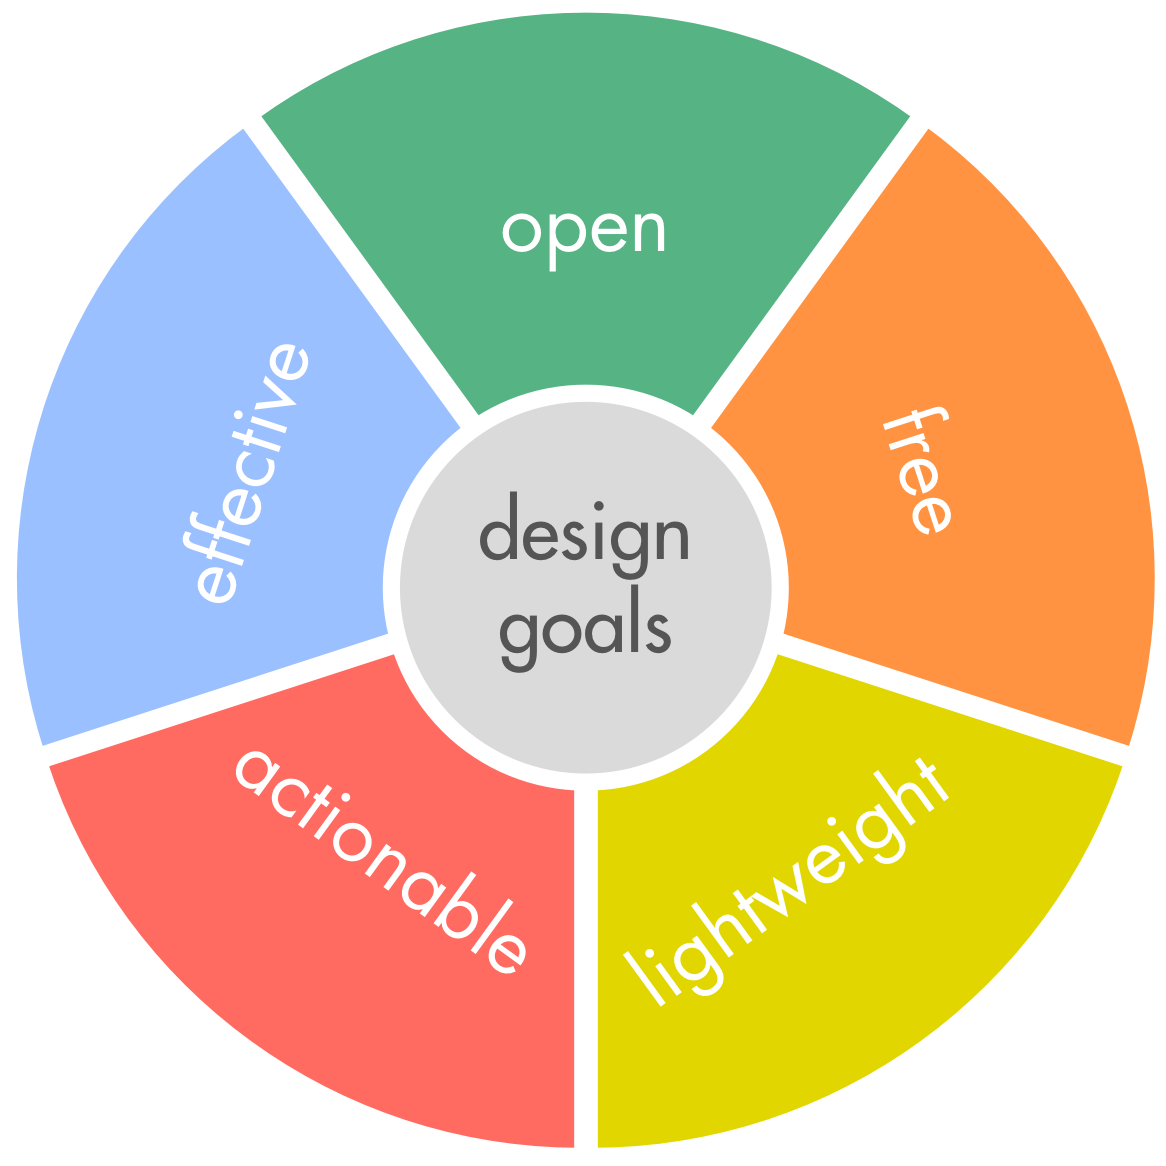
\includegraphics[keepaspectratio,width=\textwidth,height=0.75\textheight]{img/general/design-goals.png}
\end{figure}

\begin{itemize}
\item \textbf{open}:

\begin{itemize}
\item Do with it what you want

\item Take just what you need

\item Remix, extend and adapt it as you like

\end{itemize}

\item \textbf{free}

\begin{itemize}
\item Free resources

\item no hidden fees

\item no certifications

\item no small print!

\end{itemize}

\item \textbf{effective}:

\begin{itemize}
\item Principles and tools have been tried and tested for decades in many organizations.

\item need-driven, value-driven, customer focus

\end{itemize}

\item \textbf{actionable}:

\begin{itemize}
\item There's something that YOU can use right now, regardless of your unique context

\item Sociocracy 3.0 contains lots of ideas you can try out within your area of influence.

\end{itemize}

\item \textbf{lightweight}:

\begin{itemize}
\item just the essentials: Common-sense practices, bare-bone processes.

\item no stuff that gets in the way

\item no busywork

\end{itemize}

\end{itemize}

\chapter{Patterns}
\label{patterns}

\textbf{Definition}: \emph{A pattern is a template for successfully navigating a specific context.}

\begin{itemize}
\item patterns are discovered through observing many organizations as they solve problems

\item patterns may need to be adapted and evolved to suit differing contexts.

\end{itemize}

\chapter{Principles behind Sociocracy 3.0}
\label{principlesbehindsociocracy3.0}

\begin{itemize}
\item Sociocracy is built on 7 core principles

\item the core principles are also values that shape organizational culture

\item understanding these principles is paramount to adopting and adapting Sociocracy 3.0 patterns

\item practicing Sociocracy 3.0 helps people appreciate the essential value that these core principles bring, both to individuals and organizations

\end{itemize}

\begin{figure}[htbp]
\centering
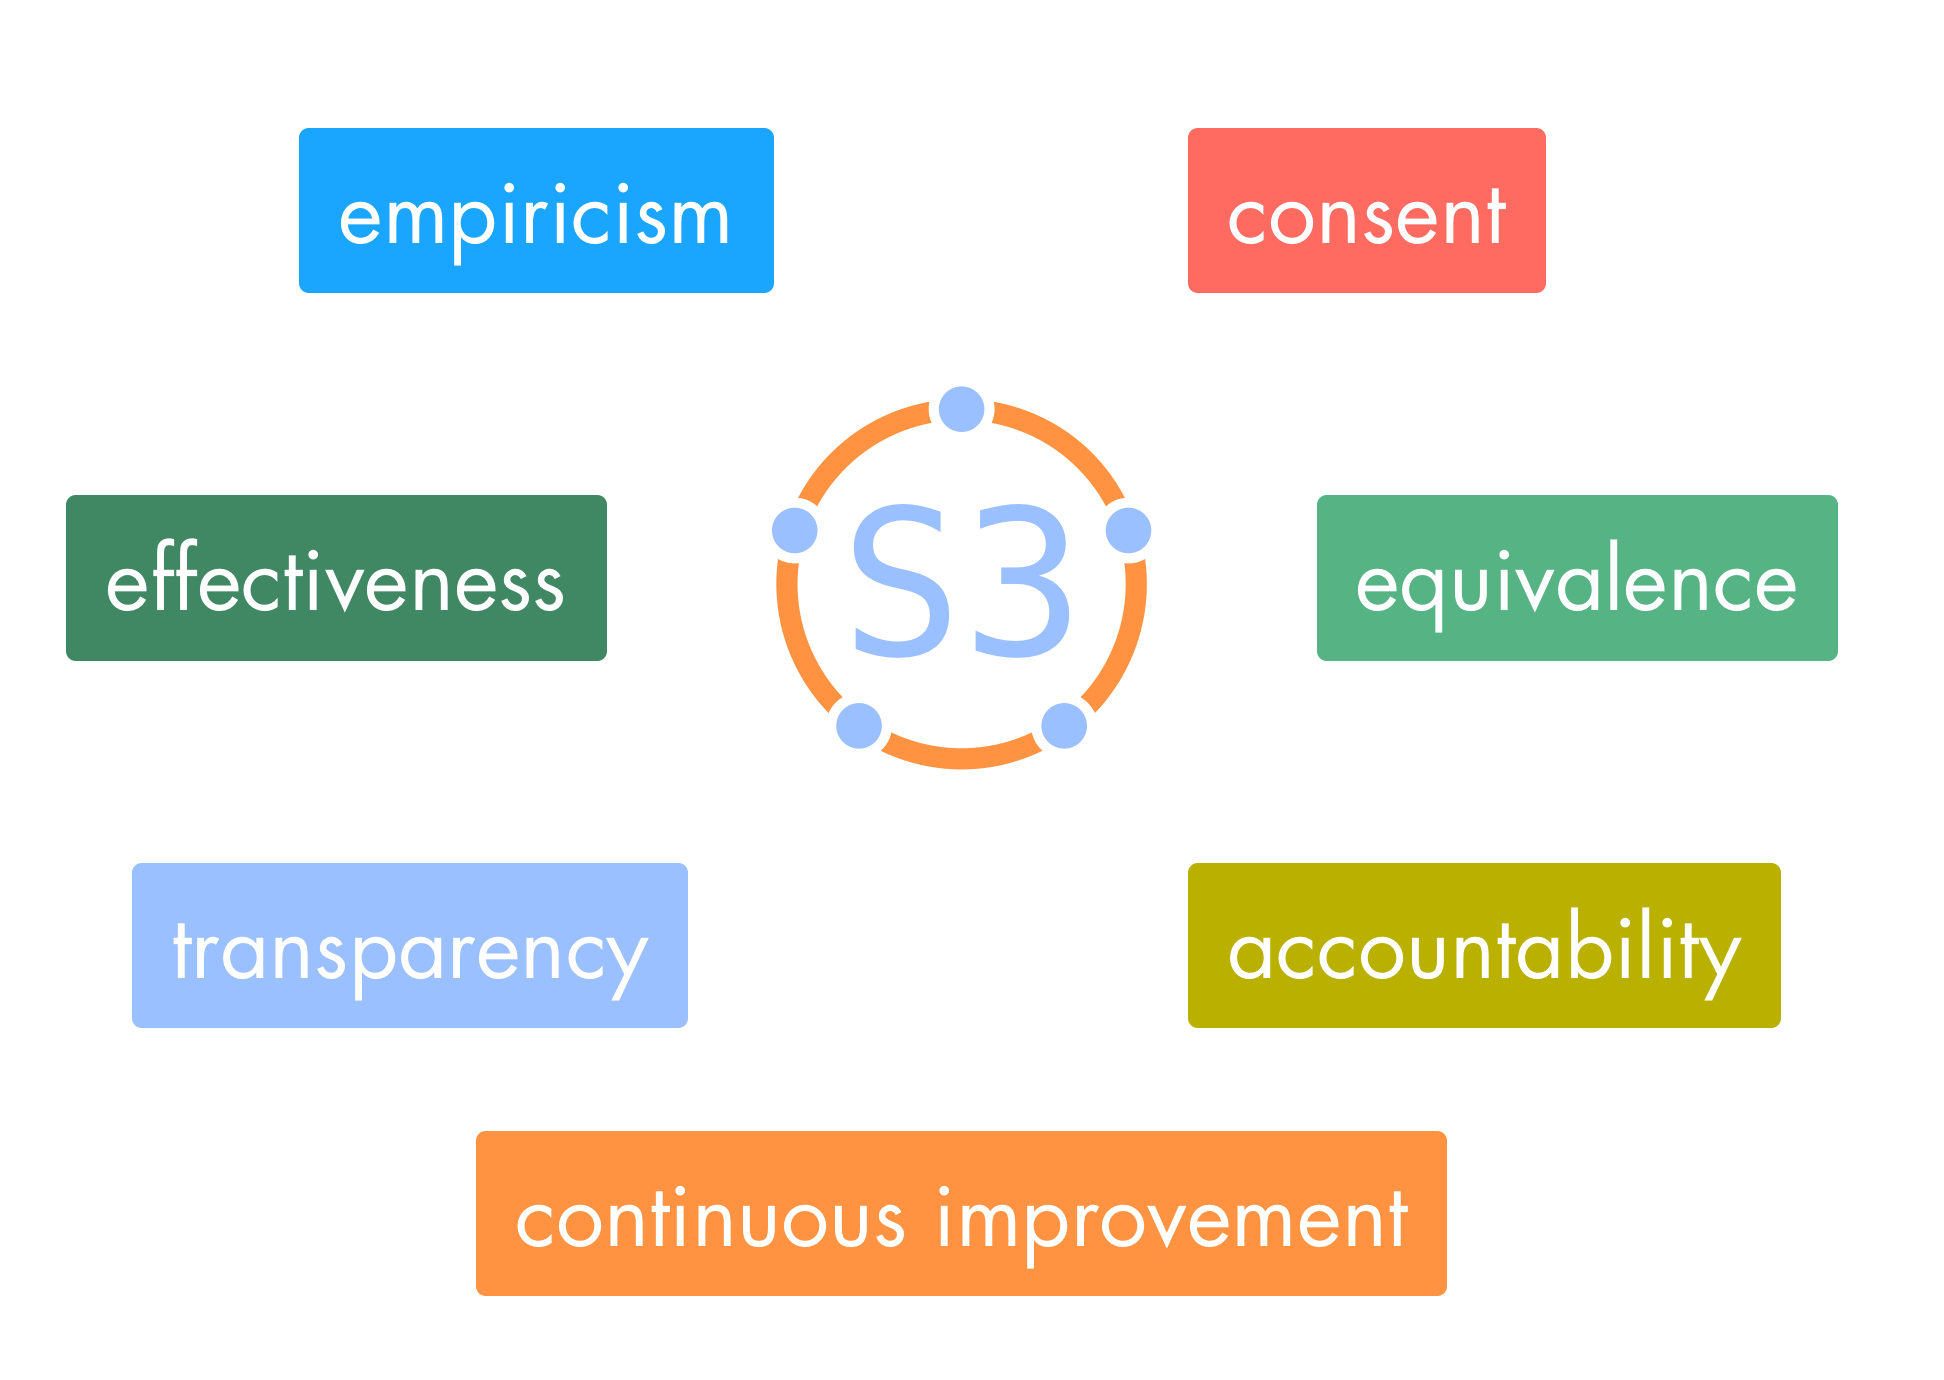
\includegraphics[keepaspectratio,width=\textwidth,height=0.75\textheight]{img/general/s3-principles-plain.png}
\end{figure}

\section{Principle: Empiricism}
\label{principle:empiricism}

\textbf{Knowledge in an organization can only be gained through experience, as it is highly dependent on context.}

\begin{itemize}
\item basis of the scientific method

\item in a complex adaptive system all knowledge is tentative

\item embrace change: continuous revision and falsification

\item reality vs. assumptions

\item learning organization

\end{itemize}

\section{Principle: Consent}
\label{principle:consent}

\textbf{Decisions are made only in the absence of reasoned objection from those affected by them.}

\begin{itemize}
\item when dealing with complexity, group wisdom exceeds individual abilities

\item deliberately seeking objections invites collective intelligence:

\begin{itemize}
\item allows for harvesting information to improve the decision

\item helps identify misunderstanding early

\item fosters support and accountability for decisions

\end{itemize}

\end{itemize}

\section{Principle: Effectiveness}
\label{principle:effectiveness}

\textbf{Devote time only to that which brings you closer to achieving your objectives.}

\begin{itemize}
\item avoid waste

\item remove impediments

\item good enough for now, safe enough to try

\end{itemize}

\section{Principle: Equivalence}
\label{principle:equivalence}

\textbf{Everyone affected by a decision has the power to withdraw consent on the basis of reasoned objection.}

\begin{itemize}
\item position, rank, function or role has no special influence in decision making

\end{itemize}

\section{Principle: Transparency}
\label{principle:transparency}

\textbf{All information is accessible to anyone in an organization. Confidentiality requires consent.}

\begin{itemize}
\item all relevant information is kept up-to-date

\item historical information is archived for reference

\end{itemize}

\section{Principle: Continuous Improvement}
\label{principle:continuousimprovement}

\textbf{Evolution is more effective than revolution (most of the time).}

\begin{itemize}
\item applies to everything (e.g. strategies, guidelines, products, skills, processes and tools)

\item respond to change by building on and transforming what is already there

\item small steps create less resistance, lower risk, and accommodate steady empirical learning

\end{itemize}

\section{Principle: Accountability}
\label{principle:accountability}

\textbf{The process of entering and keeping agreements, and managing expectations in any relationship.}

\begin{itemize}
\item an obligation or willingness to do what we agree to and to answer for when we don’t

\item a principle relevant to groups, organizations and individuals

\item a shift from being \emph{held to account}, and towards a culture of \emph{self-accountability}

\end{itemize}

\chapter{Organizations}
\label{organizations}

An organization is defined by its values, driver and strategy.

\begin{itemize}
\item an organizations values define \textbf{culture} and set parameters for \textbf{action}

\item an organizations \textbf{existence} is motivated by its driver

\item an organizations \textbf{service} is defined by its strategy

\item organizations are aligned towards values, driver and strategy

\item with Sociocracy 3.0, \emph{purpose} is implicit (to satisfy drivers)

\item to transition towards Sociocracy 3.0 an organization:

\begin{itemize}
\item identifies values and driver of the organization

\item incorporates vision, mission, aims or objectives in the strategy

\item seeks out drivers for all existing policy and agreements (including circles and roles)

\end{itemize}

\end{itemize}

\part{The Patterns}
\label{thepatterns}

\chapter{Making And Evolving Agreements}
\label{makingandevolvingagreements}

{\ldots}

\section{Agreements}
\label{agreements}

We respond to drivers through agreements.

\textbf{Definition:} \emph{A agreement is an agreed upon guideline, pattern, process or protocol designed to guide the flow of value.}

\begin{itemize}
\item agreements are created in order to satisfy drivers

\item agreements are the \textbf{accountability of the circle} that created them

\item each agreement includes \textbf{evaluation criteria} and is subject to \textbf{regular review}

\begin{itemize}
\item review dates are specific to each agreement

\item agreements are reviewed in context to its driver

\end{itemize}

\end{itemize}

\begin{figure}[htbp]
\centering
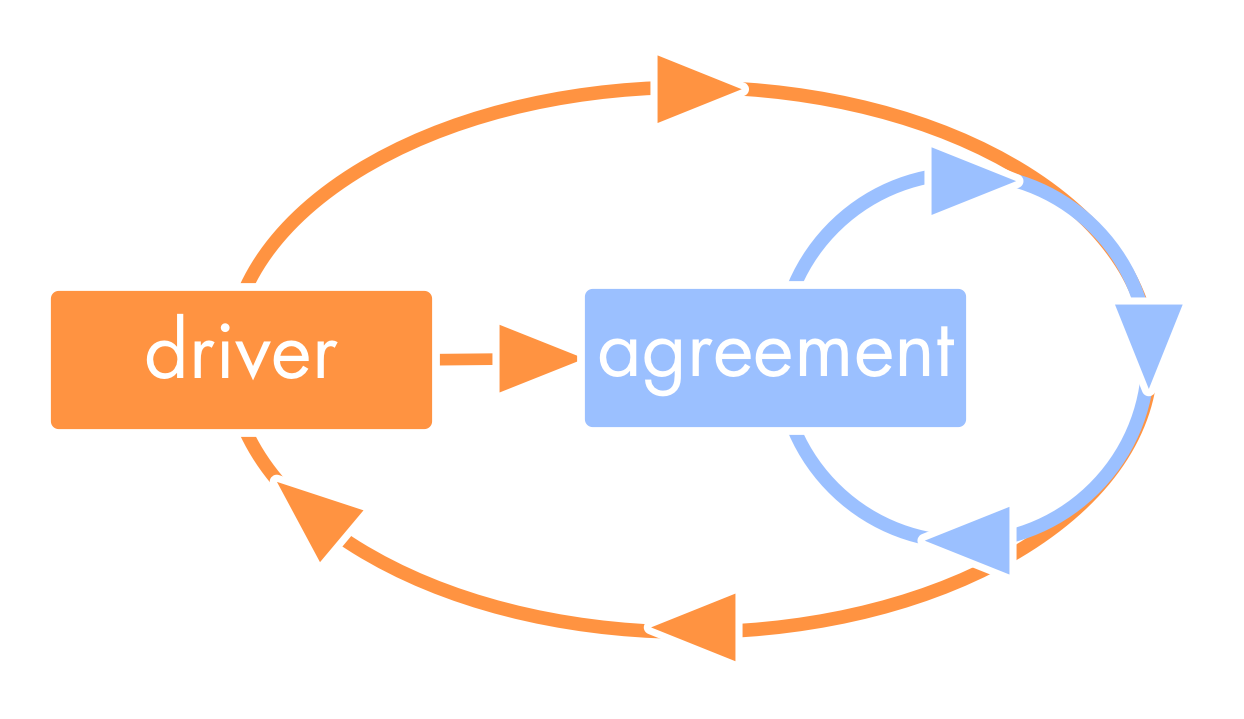
\includegraphics[keepaspectratio,width=\textwidth,height=0.75\textheight]{img/tension-driver-domain/driver-agreement-improvement.png}
\end{figure}

\subsection{Template for Agreements}
\label{templateforagreements}

\begin{figure}[htbp]
\centering
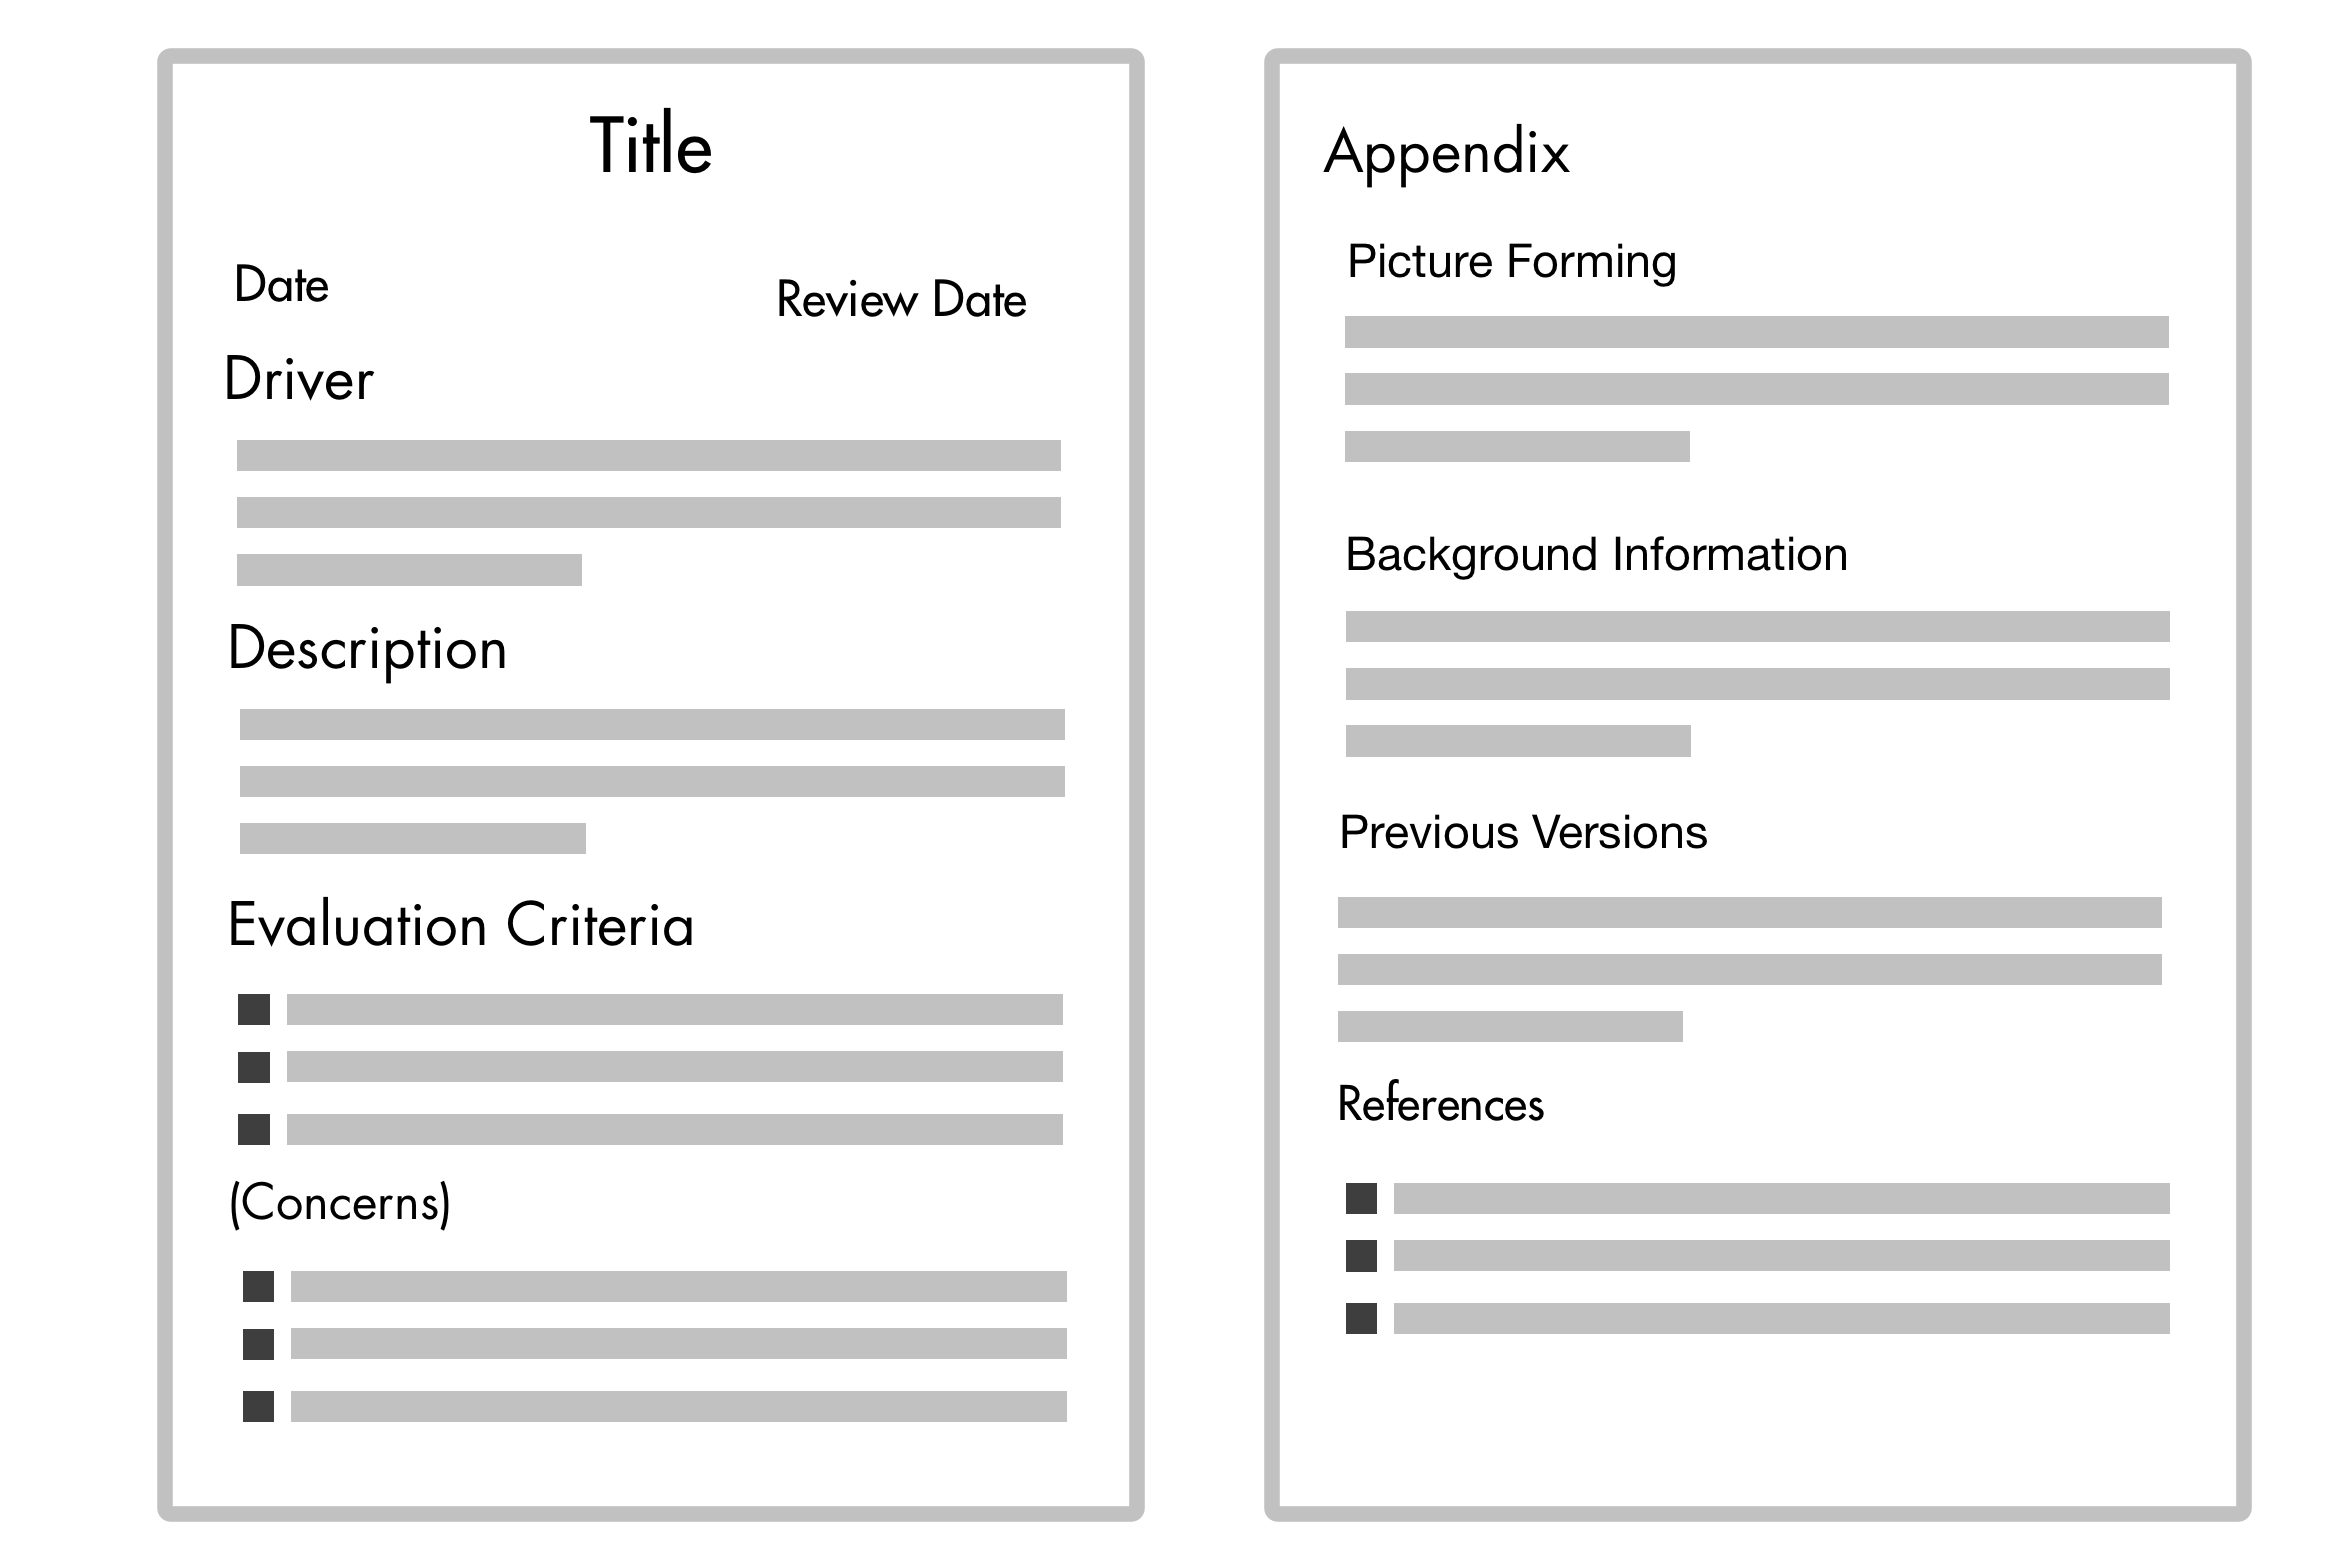
\includegraphics[keepaspectratio,width=\textwidth,height=0.75\textheight]{img/agreements/agreement-template.png}
\end{figure}

\section{Circle}
\label{circle}

A circle{\ldots}

\begin{itemize}
\item {\ldots}is the basic building block of an organization

\item {\ldots}is a group of people gathered around a driver (permanent or temporary)

\item {\ldots}makes all agreements by consent

\item {\ldots}is accountable for its own development

\end{itemize}

\textbf{Definition:} \emph{A circle is a semi-autonomous, self-organizing and self-governing group of people gathering around a driver.}

\begin{figure}[htbp]
\centering
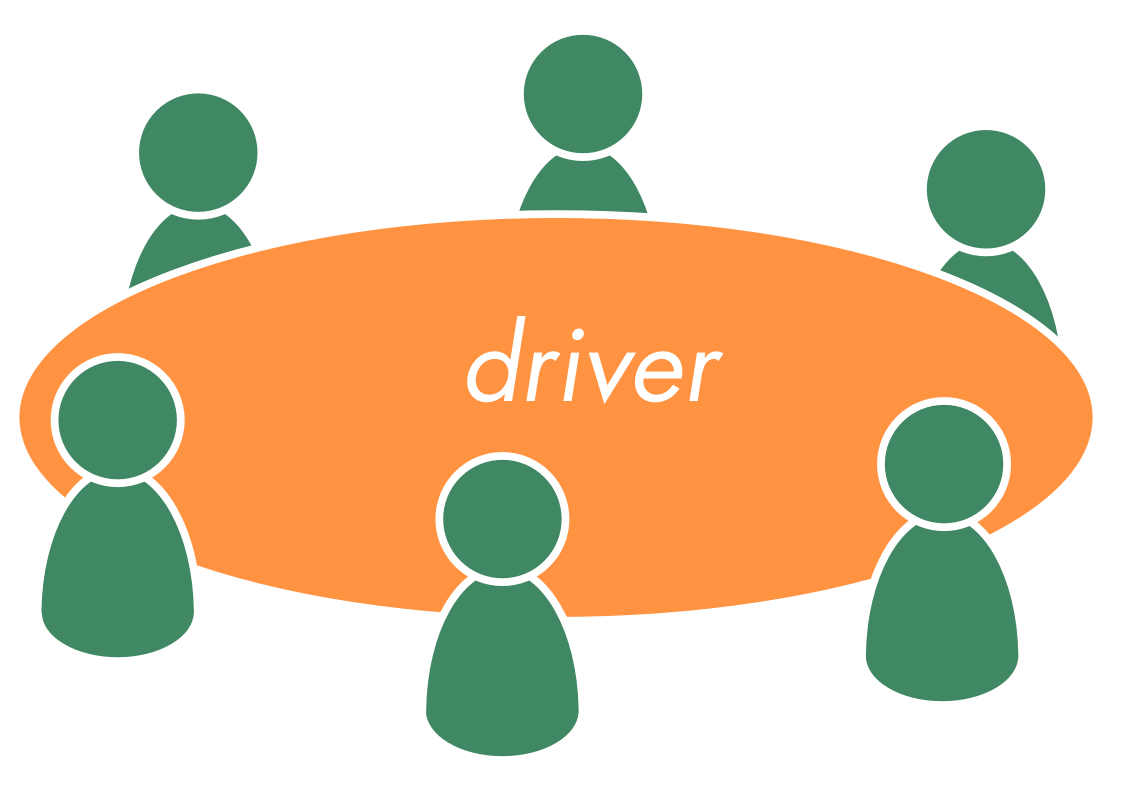
\includegraphics[keepaspectratio,width=\textwidth,height=0.75\textheight]{img/circle/circle-driver.png}
\end{figure}

\begin{itemize}
\item {\ldots}\textbf{semi-autonomous}:

\begin{itemize}
\item each has a unique driver and can create value independently

\end{itemize}

\item {\ldots}\textbf{self-organizing}:

\begin{itemize}
\item independent in organizing day-to-day-work

\end{itemize}

\item {\ldots}\textbf{self-governing}:

\begin{itemize}
\item independent in creating strategy and agreements

\end{itemize}

\end{itemize}

\section{Consent Decision Making}
\label{consentdecisionmaking}

\begin{itemize}
\item Consent is the absence of objections

\begin{itemize}
\item everyone affected by a decision can ``live with it''

\item consent is not consensus with unanimity

\end{itemize}

\item Consent is used to make and evolve all agreements in a circle

\item Objections stop proposals becoming agreements

\item Withholding objections could harm the aims of a group or organization

\item Being able to raise objections at any time means that proposals only need to be \emph{good enough for now, safe enough to try}

\item Every agreement has a review date

\end{itemize}

Consent Decision Making{\ldots}

\begin{itemize}
\item is a facilitated decision making process

\item deliberately harvests reasoned objections in order to integrate the wisdom they contain in proposals or existing agreements

\item helps balance equivalence and effectiveness

\item experienced groups can move quickly through the stages of Consent Decision Making

\end{itemize}

\subsection{Harvesting Objections to Capture Emergent Wisdom}
\label{harvestingobjectionstocaptureemergentwisdom}

\begin{figure}[htbp]
\centering
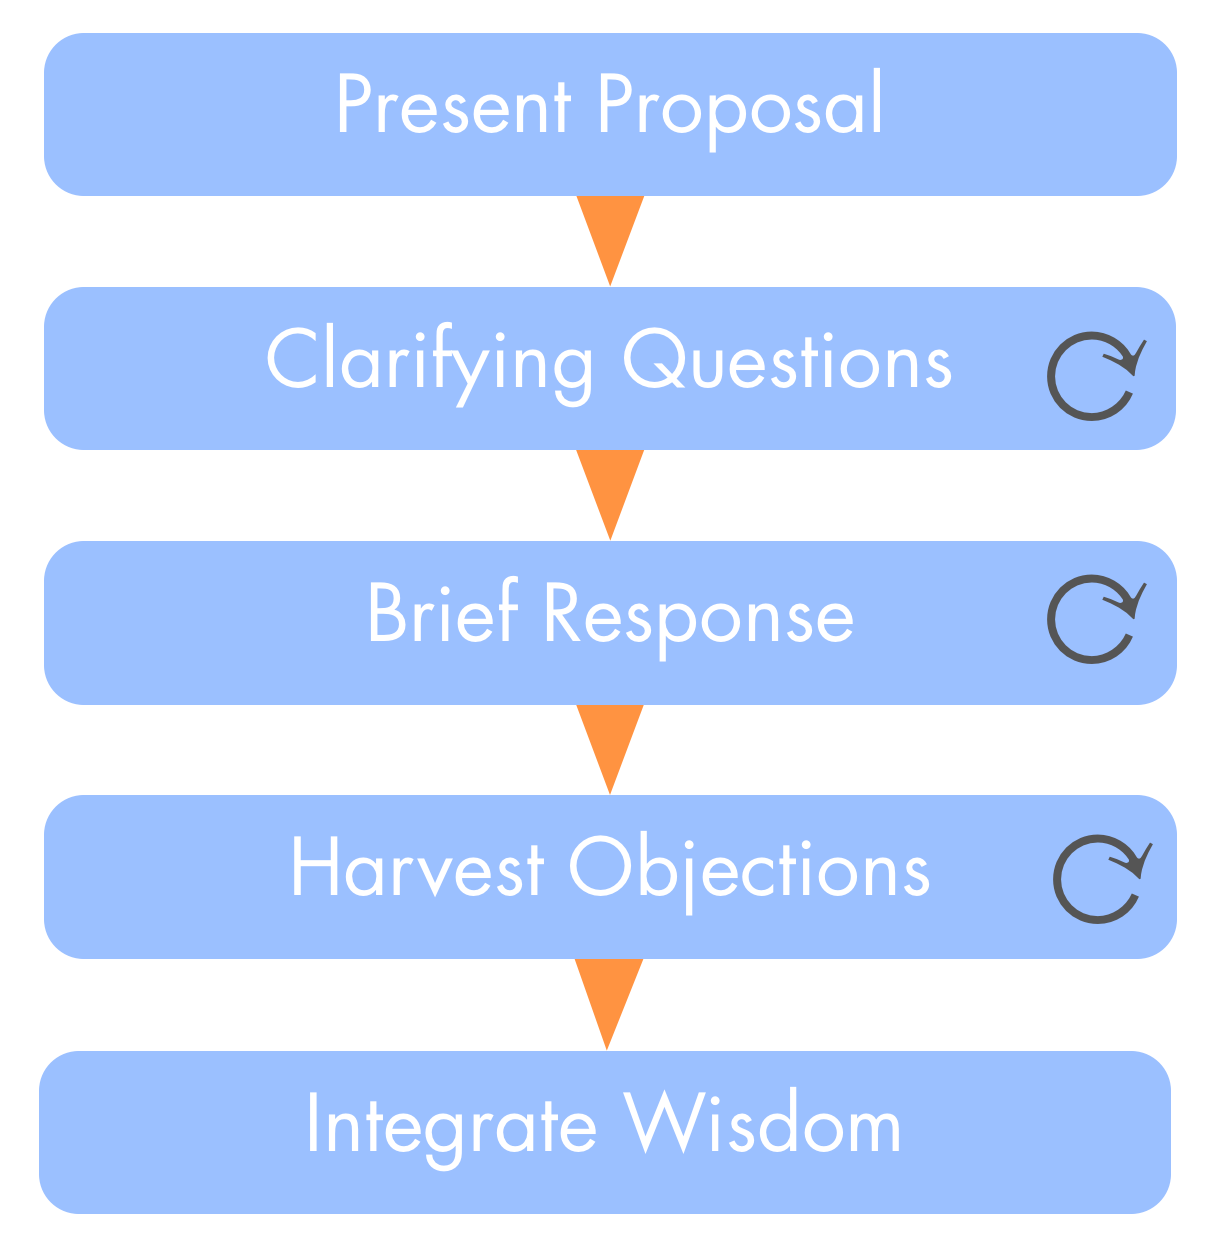
\includegraphics[keepaspectratio,width=\textwidth,height=0.75\textheight]{img/agreements/cdm-condensed.png}
\end{figure}

\section{Deliverables}
\label{deliverables}

{\ldots}

\section{Driver}
\label{driver}

\textbf{Definition:}: \emph{A driver is that which motivates us into action: what is happening in a specific situation and what’s needed.}

\section{Responses to a Driver}
\label{responsestoadriver}

\begin{itemize}
\item the response to a driver always involves the \textbf{adaptation of an existing agreement, or creation of a new one}, including:

\begin{itemize}
\item changing the plan: adding a task or project

\item adaptation or creation of a role

\item creation of a new circle

\begin{itemize}
\item driver review is delegated to new circle

\end{itemize}

\end{itemize}

\end{itemize}

\subsection{Drivers Are Subject to Regular Review}
\label{driversaresubjecttoregularreview}

\begin{itemize}
\item Is the description of the current reality correct?

\item Do we still associate the same needs with the current reality?

\item Is the driver still within our domain?

\item Is the driver still relevant?

\end{itemize}

\subsection{Sociocracy 3.0 and Lean Thinking}
\label{sociocracy3.0andleanthinking}

\subsubsection{Value and Waste}
\label{valueandwaste}

\textbf{Definition}: \emph{The importance, worth or usefulness of something for satisfaction of a driver.}

\textbf{Value}:

\begin{itemize}
\item value is \textbf{not} an \textbf{inherent} property as it only exists in relation to a driver

\item value can be quantified by \textbf{measuring the progression} towards satisfaction of a driver

\begin{itemize}
\item value is not necessarily expressed in currency or time

\end{itemize}

\item \textbf{continuous improvement of processes is focused on optimizing the flow of value through an organization}

\end{itemize}

\textbf{Definition:} \emph{Waste is anything not necessary (essential) for - or standing in the way of - effective satisfaction of a driver.}

Adopting the concept of value and waste makes many tools and ideas from \textbf{lean production} and \textbf{lean software development} available to support organizations running on Sociocracy 3.0:

\begin{itemize}
\item value stream mapping

\item various strategies for eliminating waste

\item the Kanban Method

\end{itemize}

\subsubsection{Waste and Continuous Improvement}
\label{wasteandcontinuousimprovement}

\begin{itemize}
\item Establishing a process for ongoing elimination of waste enables natural evolution of an organization towards greater effectiveness

\item Adaptation to changing environment is built into the process

\end{itemize}

\subsubsection{Identifying Waste}
\label{identifyingwaste}

\begin{figure}[htbp]
\centering
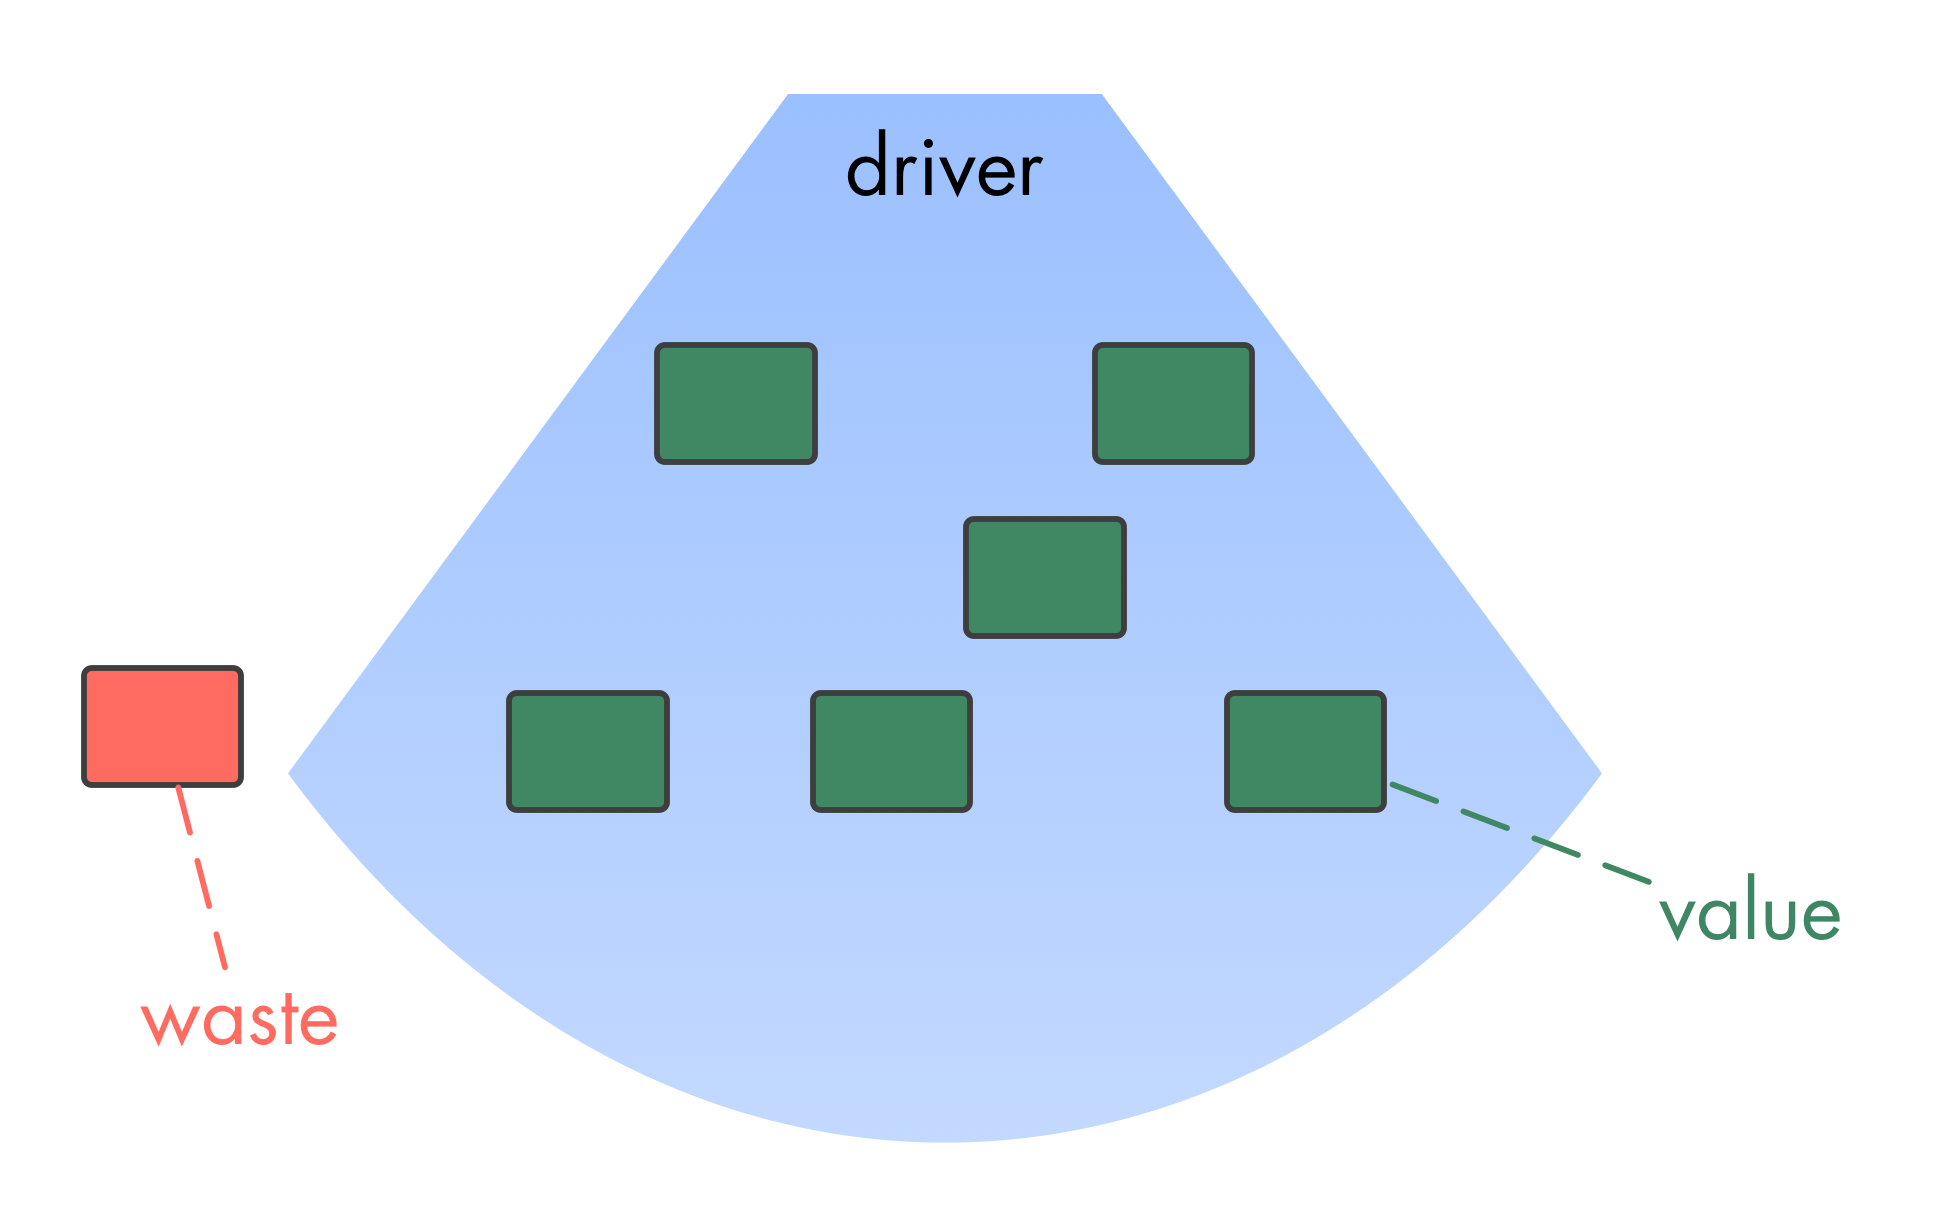
\includegraphics[keepaspectratio,width=\textwidth,height=0.75\textheight]{img/workflow-and-value/drivers-value-waste.png}
\end{figure}

\begin{itemize}
\item waste exist in many different forms and on different levels of abstraction

\begin{itemize}
\item tasks, processes, organizational structure, mental models{\ldots}

\end{itemize}

\item some tensions reveal waste

\item learning to identify waste is a journey

\begin{itemize}
\item along the way we also learn how to evolve our drivers

\end{itemize}

\end{itemize}

\section{Evaluate Agreements}
\label{evaluateagreements}

{\ldots}

\section{Evaluation Criteria}
\label{evaluationcriteria}

\begin{figure}[htbp]
\centering
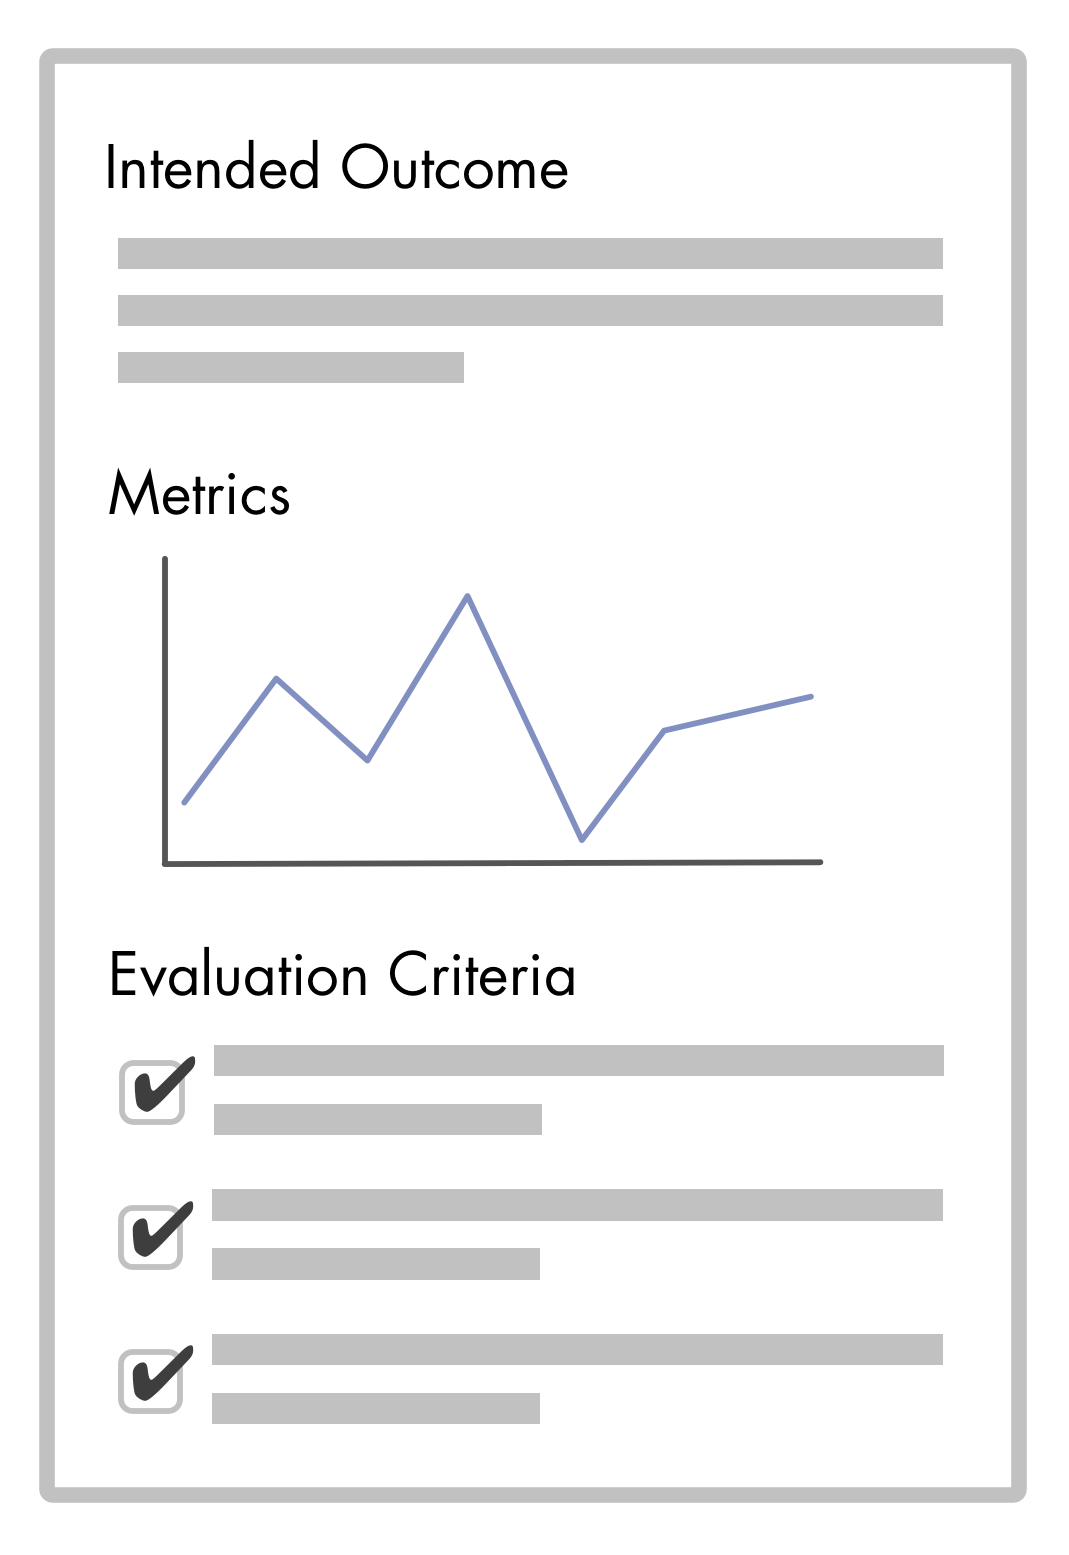
\includegraphics[keepaspectratio,width=\textwidth,height=0.75\textheight]{img/agreements/outcome-and-criteria.png}
\end{figure}

\section{Intended Outcome}
\label{intendedoutcome}

\begin{figure}[htbp]
\centering
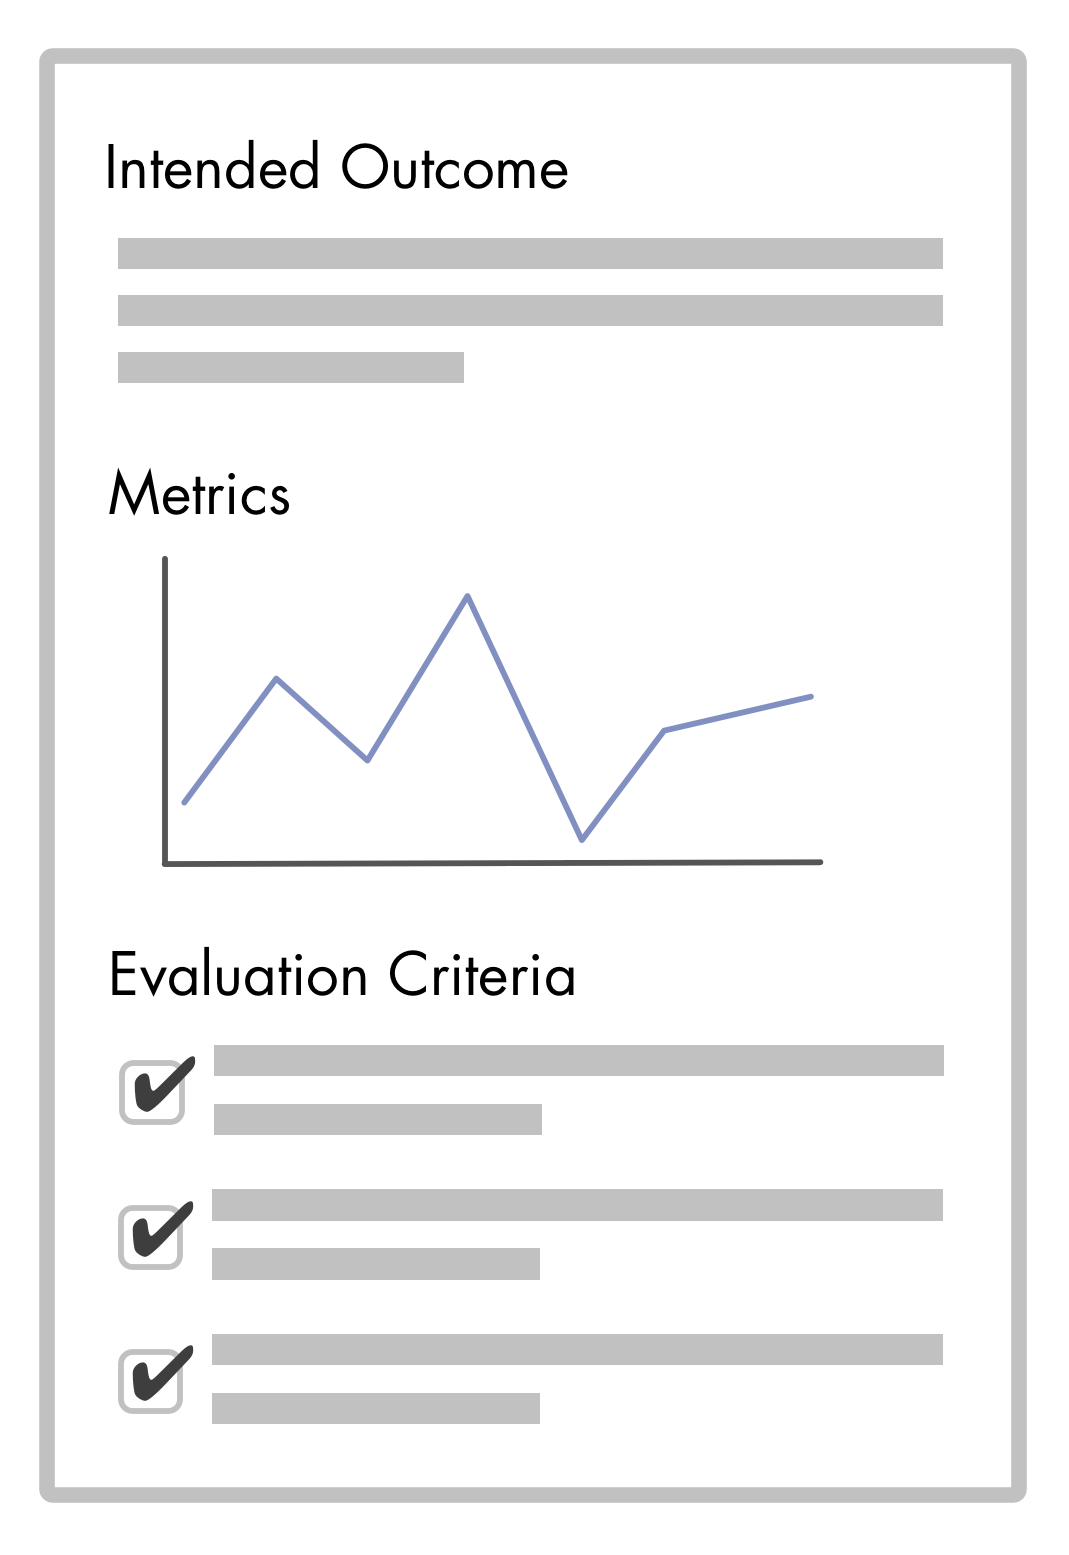
\includegraphics[keepaspectratio,width=\textwidth,height=0.75\textheight]{img/agreements/outcome-and-criteria.png}
\end{figure}

\section{Objections}
\label{objections}

\textbf{Definition:} \emph{An objection is a reason why doing what is proposed stands in the way of (more) effective satisfaction of an existing driver.}

In sociocracy we deliberately seek objections as they reveal
wisdom that can be used to improve proposals and agreements.

Objections{\ldots}

\begin{itemize}
\item {\ldots}are gifts

\item {\ldots}reveal wisdom seeking expression into the consciousness of a circle

\item {\ldots}reveal opportunities or impediments

\item {\ldots}emerge through individuals and belong to the whole circle

\item we love objections in sociocracy

\end{itemize}

\subsection{Questions That Help to Validate Objections}
\label{questionsthathelptovalidateobjections}

\begin{itemize}
\item Does the objection relate to this specific proposal or agreement?

\item Does this objection reveal how a (proposed or existing) \textbf{agreement}{\ldots}

\begin{itemize}
\item {\ldots}jeopardizes the satisfaction of a driver?

\item {\ldots}is in conflict with the organization's values?

\item {\ldots}prevents or diminishes someone's contribution to satisfying a driver?

\item {\ldots}can be improved significantly?

\end{itemize}

\end{itemize}

\section{Concerns{\ldots}}
\label{concerns...}

\begin{itemize}
\item {\ldots}are not objections

\item {\ldots}don't stop us from making agreements

\item {\ldots}often contain wisdom

\item {\ldots}can be recorded in the logbook

\begin{itemize}
\item {\ldots}to further evolve agreements

\item {\ldots}to set evaluation criteria (including review date)

\end{itemize}

\end{itemize}

\section{Proposal Forming}
\label{proposalforming}

Proposal Forming{\ldots}

\begin{itemize}
\item {\ldots}is similar to condensed design thinking process

\item {\ldots}taps the collective intelligence of a group

\item {\ldots}involves people in co-creating agreements

\item {\ldots}fosters accountability and a sense of ownership

\end{itemize}

\begin{figure}[htbp]
\centering
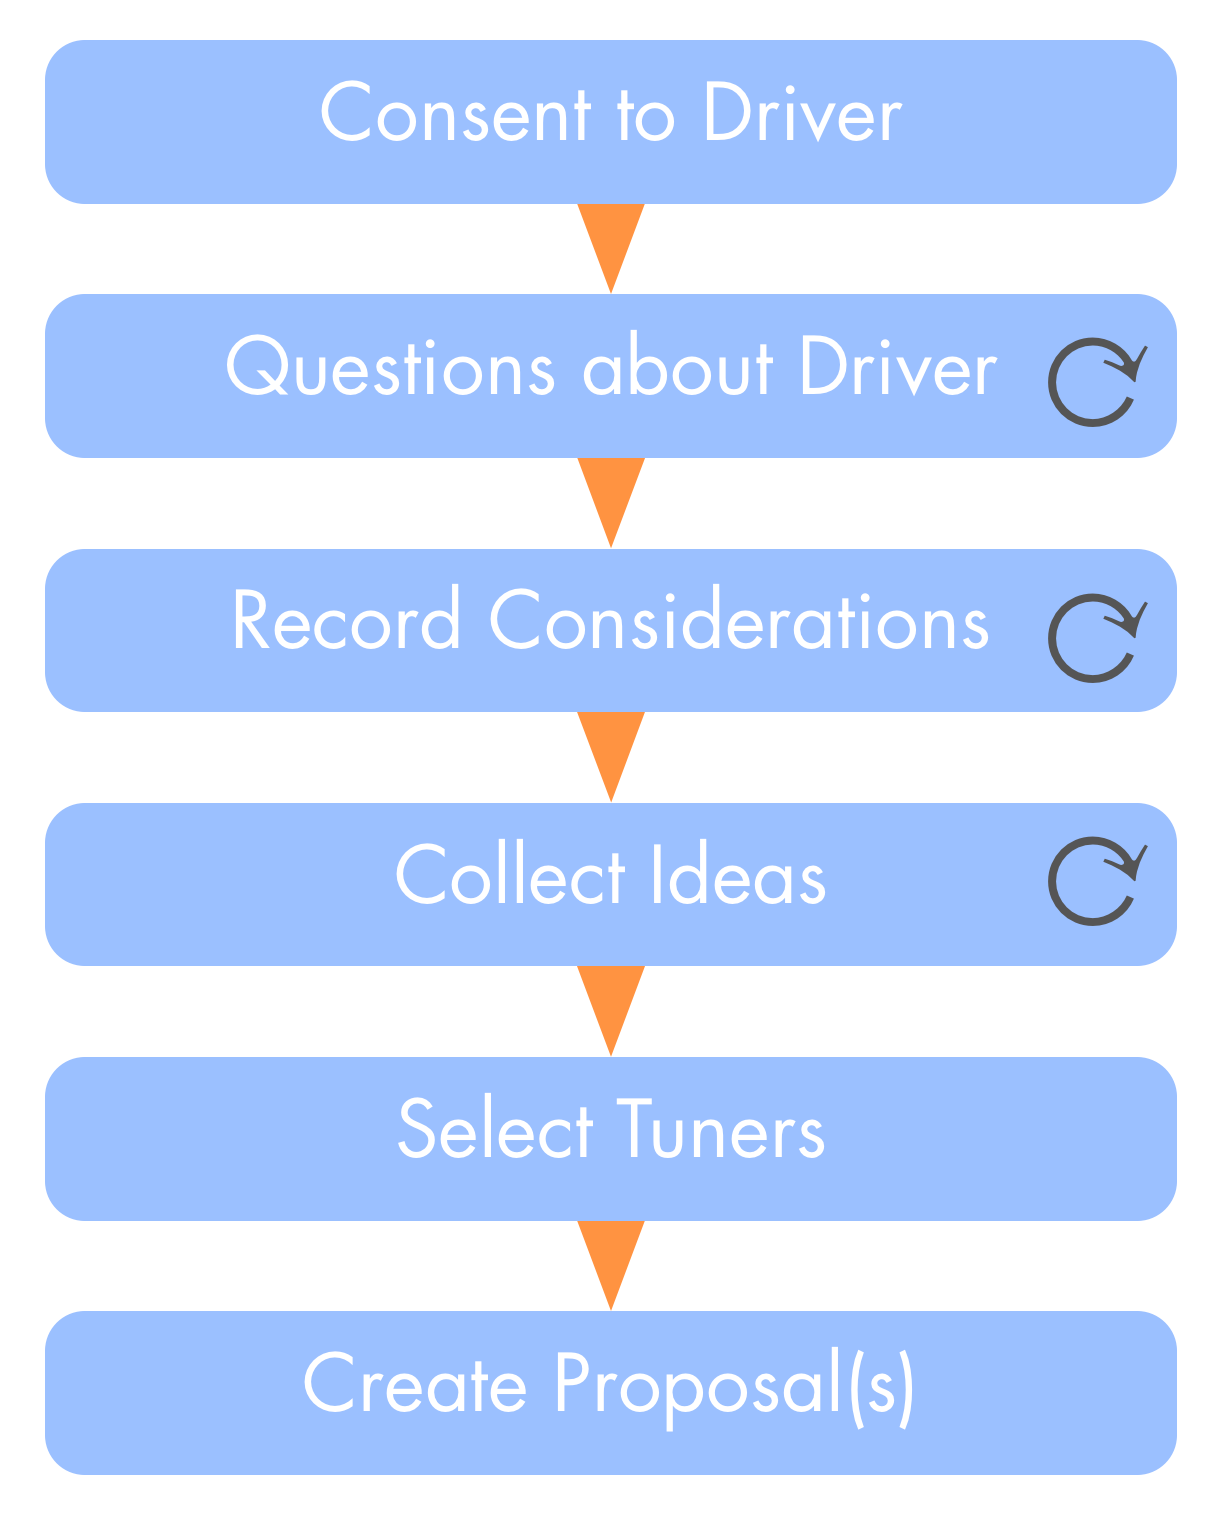
\includegraphics[keepaspectratio,width=\textwidth,height=0.75\textheight]{img/agreements/proposal-forming-medium.png}
\caption{Co-Creating a Response to a Drivers}
\end{figure}

\subsection{Proposal Forming Process}
\label{proposalformingprocess}

\begin{enumerate}
\item \textbf{Identify} the driver

\item \textbf{Consider}: Collect considerations as questions that reveal the scope of the issue

\item \textbf{Create}: Gather ingredients\slash ideas for solutions

\item \textbf{Refine}: Design a proposal from some or all of the ingredients

\item \textbf{Review}: process with consent decision making

\end{enumerate}

\section{Qualifying Drivers}
\label{qualifyingdrivers}

** {\ldots}in order to avoid action bias**

\begin{quote}

\emph{Between stimulus and response there is a space. In that space is our power to choose our response. In our response lies our growth and our freedom.} (Viktor E. Frankl)
\end{quote}

We consider why, how and when to respond to a stimulus, instead of defaulting to action.

\section{Resolve Objections}
\label{resolveobjections}

\section{Methods for Resolving Objections}
\label{methodsforresolvingobjections}

\begin{itemize}
\item ask proposal owner

\item ask member with objection to amend proposal

\item facilitator amends proposal

\item ``How would you solve this'' – round

\item Brief Dialogue – 2 or 3 people

\item Brief group discussion

\item refer to proposal forming

\item drop the proposal

\item Re-work – Send back to higher \slash  lower circle

\item Form a temporary circle to review, research, revise

\end{itemize}

\section{Strategy}
\label{strategy}

\begin{figure}[htbp]
\centering
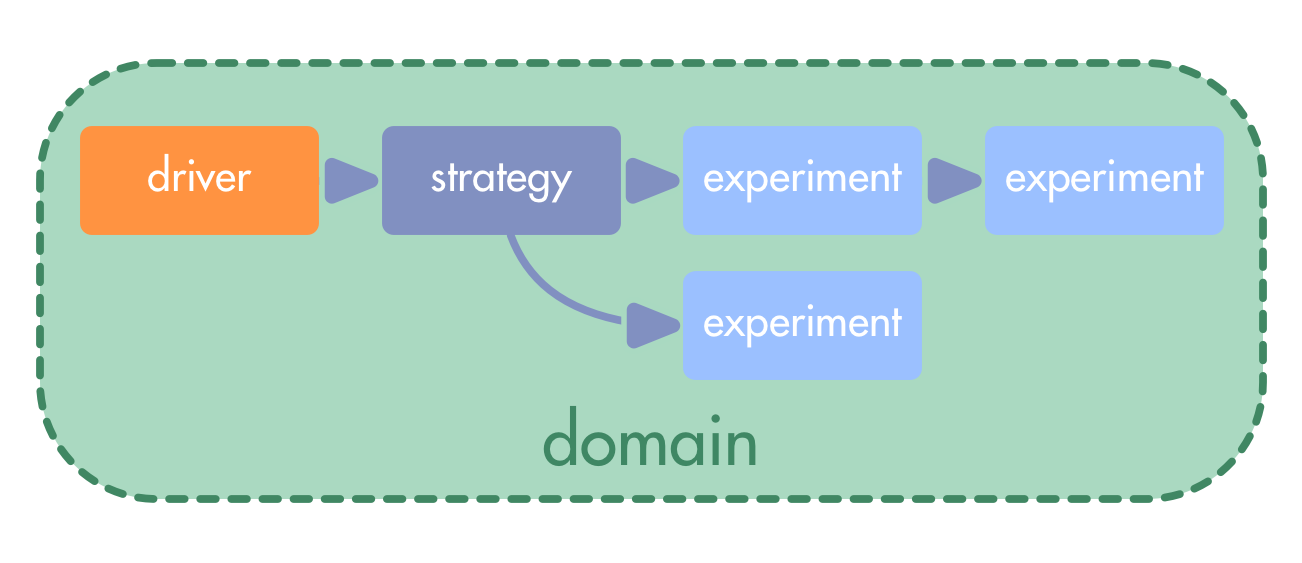
\includegraphics[keepaspectratio,width=\textwidth,height=0.75\textheight]{img/drivers-and-subdrivers/driver-and-domains.png}
\end{figure}

\section{Those Affected Decide}
\label{thoseaffecteddecide}

{\ldots}

\chapter{Navigation}
\label{navigation}

Governance is the process of creating and evolving agreements in response to drivers.

\section{Governance Backlog}
\label{governancebacklog}

{\ldots}

\section{Governance Meeting}
\label{governancemeeting}

Circles meet at regular intervals to create and evolve agreements in response to drivers.

\begin{itemize}
\item usually \ensuremath{\sim}60 min

\item regular cadence, usually 2--4 weeks

\end{itemize}

\subsection{Navigation Meeting Structure}
\label{navigationmeetingstructure}

\begin{itemize}
\item Opening Round

\begin{itemize}
\item attune to one another and to the driver the circle serves

\end{itemize}

\item Administrative Matters

\begin{itemize}
\item consent to last minutes, dates, consent to agenda

\end{itemize}

\item Agenda Items

\begin{itemize}
\item Short Reports

\item Processing Tensions

\item Proposal Forming and Consent to Proposals

\item Review of Agreements, Strategy and Driver

\item Defining Roles and Selecting People for Roles

\item Consent to Role Improvement Plans

\end{itemize}

\item Closing Round

\begin{itemize}
\item evaluation of meeting and results, future agenda items

\end{itemize}

\end{itemize}

\section{Navigating via tension}
\label{navigatingviatension}

\textbf{Definition}: \emph{A tension is the subjective experience of contradiction between reality and that which we desire or anticipate.}

\begin{itemize}
\item individuals act as sensors (nerve endings) for the organization

\item tension is experienced whenever our perception of our environment is in conflict with:

\begin{itemize}
\item that which we desire or had anticipated

\item our values (and principles)

\end{itemize}

\item problems, challenges, and feelings of unease are all tensions

\end{itemize}

\begin{figure}[htbp]
\centering
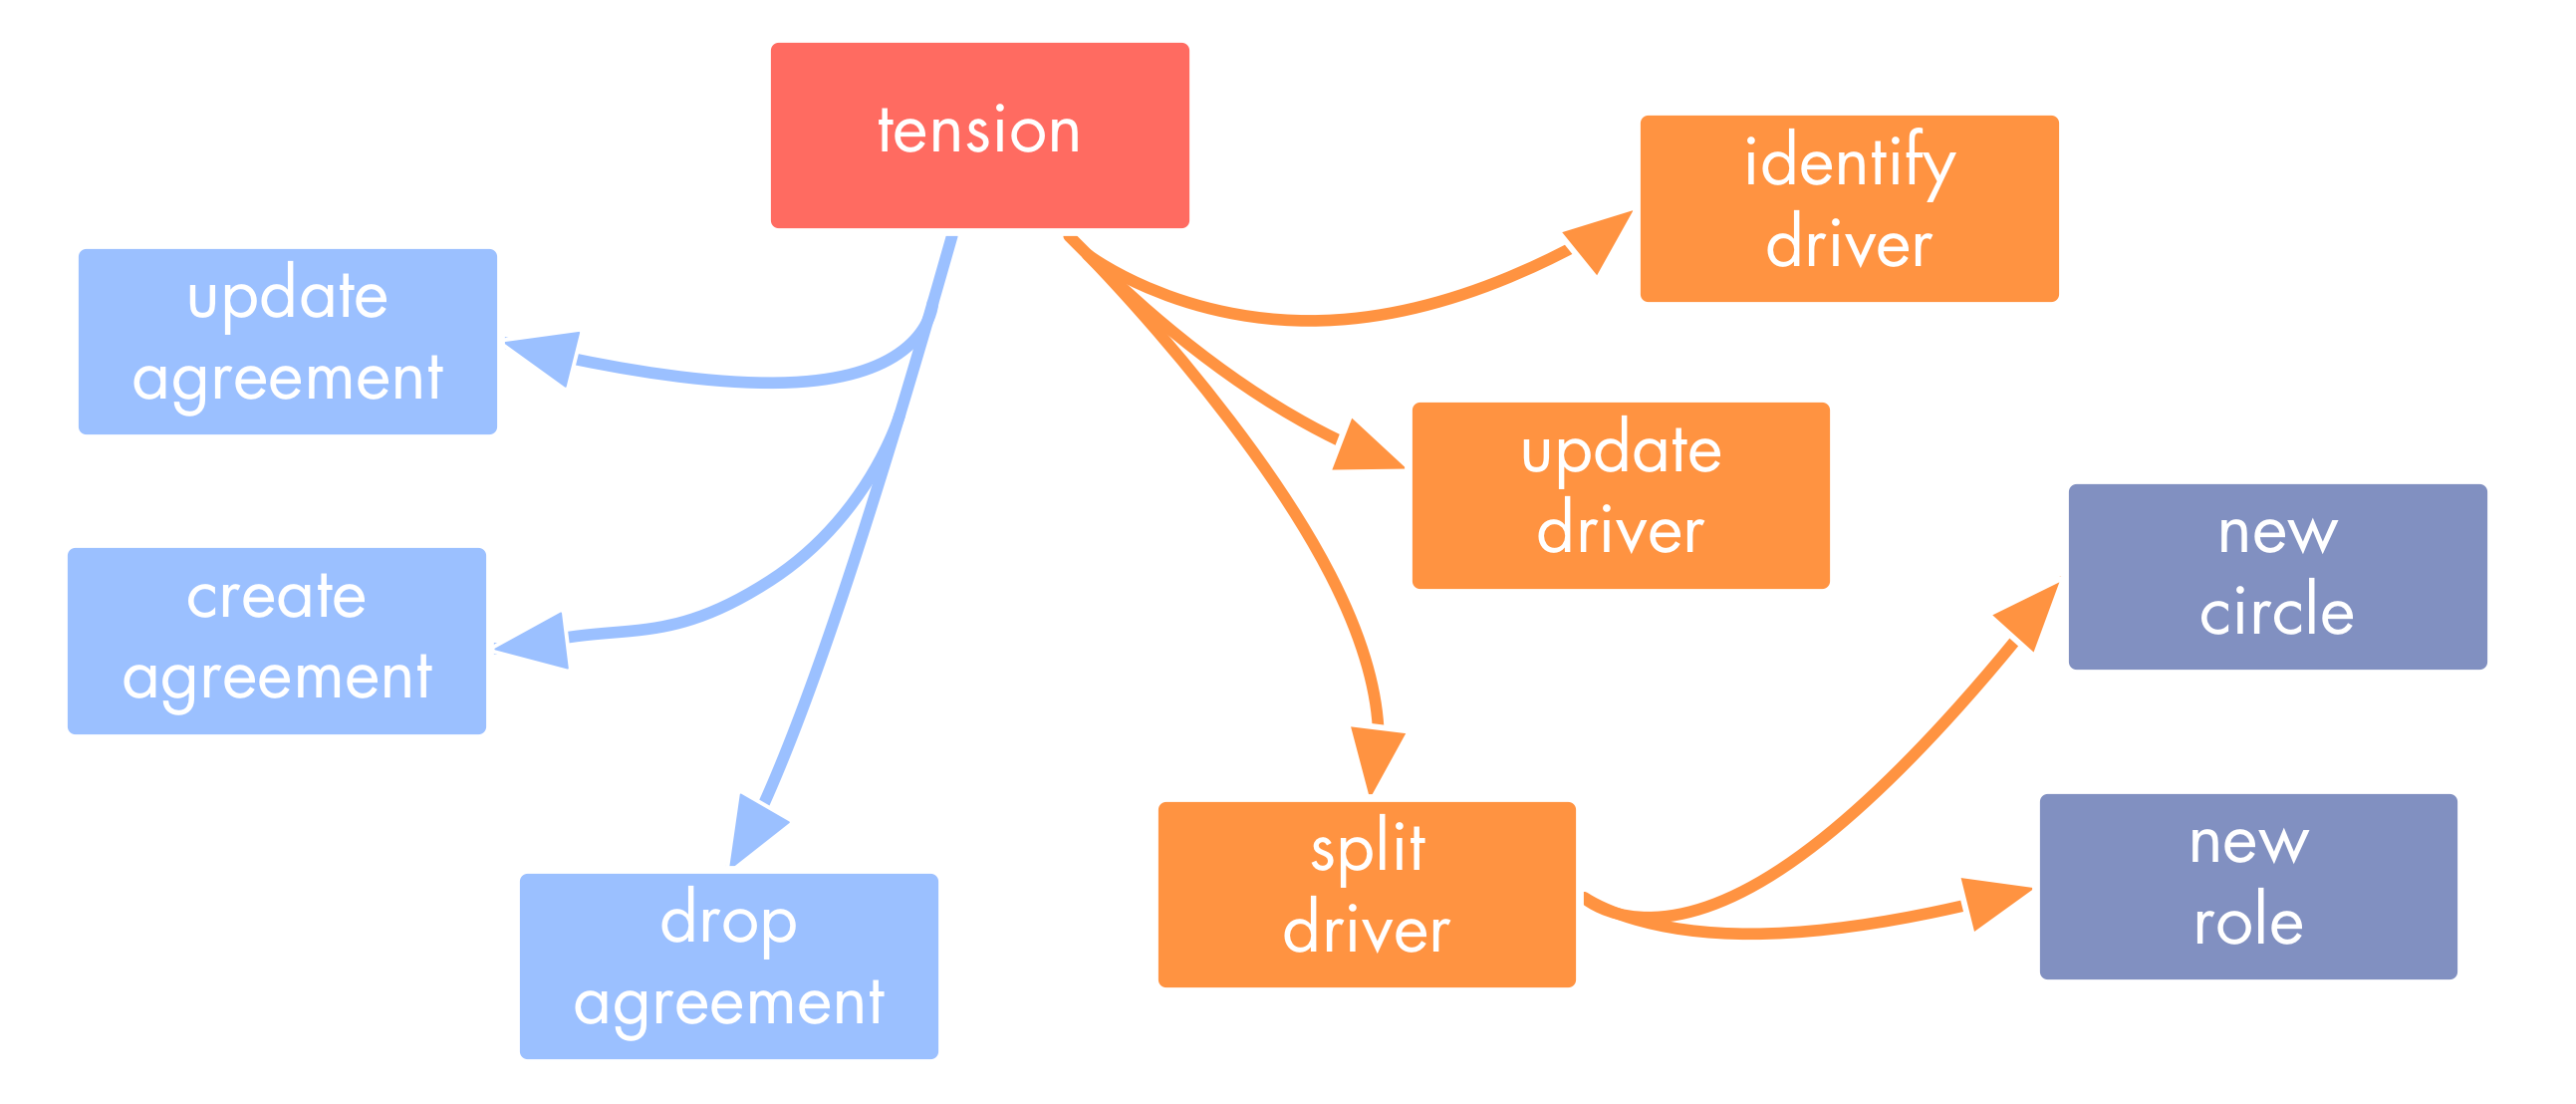
\includegraphics[keepaspectratio,width=\textwidth,height=0.75\textheight]{img/tension-driver-domain/navigate-via-tensions.png}
\end{figure}

\subsection{From Tension to Driver}
\label{fromtensiontodriver}

\begin{itemize}
\item investigating tension leads to the discovery of drivers

\item to identify a possible driver behind a tension we:

\begin{itemize}
\item \textbf{describe} the current reality

\item \textbf{identify} the needs we associate with that reality

\end{itemize}

\item in the process, we resolve some tensions as \textbf{misunderstandings}

\item we validate drivers

\begin{itemize}
\item some tensions are \textbf{outside the domain} we can address

\end{itemize}

\end{itemize}

\chapter{Effective Meetings}
\label{effectivemeetings}

{\ldots}

\section{S3 Facilitator}
\label{s3facilitator}

\begin{figure}[htbp]
\centering
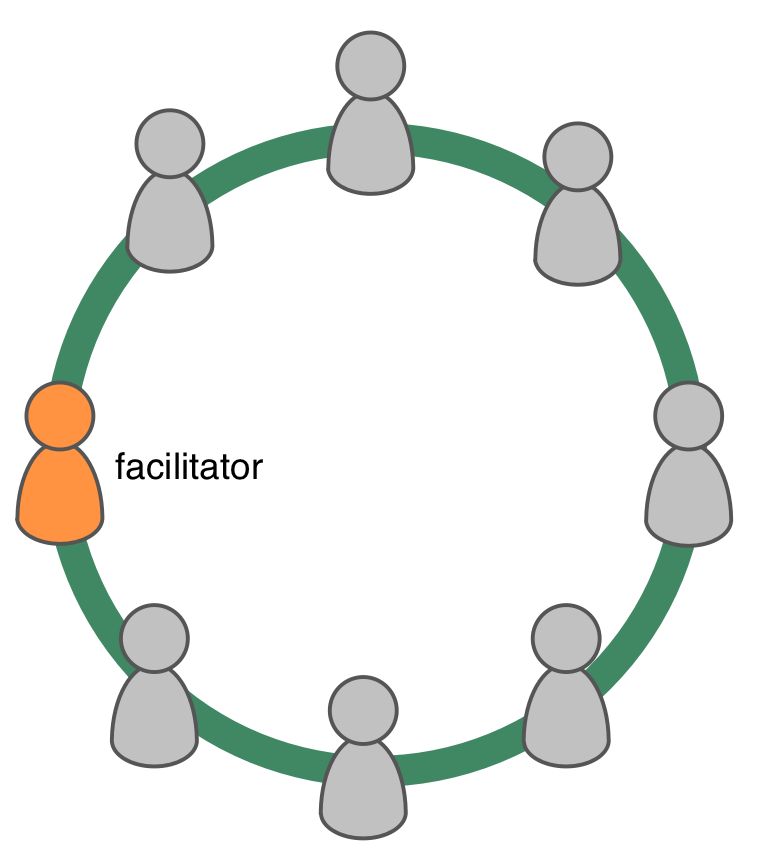
\includegraphics[keepaspectratio,width=\textwidth,height=0.75\textheight]{img/circle/facilitator.png}
\end{figure}

\section{Artful Participation}
\label{artfulparticipation}

{\ldots}

\section{Logbook}
\label{logbook}

\begin{itemize}
\item Organization:

\begin{itemize}
\item driver, strategy

\item organizational values

\item organizational structure

\item agreements

\end{itemize}

\item Circle:

\begin{itemize}
\item driver, strategy

\item agreements

\item role definitions and role improvement plans

\end{itemize}

\item Personal logbooks

\begin{itemize}
\item role descriptions

\item tasks

\item personal strategy and personal policy

\end{itemize}

\end{itemize}

\section{Logbook Keeper}
\label{logbookkeeper}

{\ldots}

\section{Meeting Evaluation}
\label{meetingevaluation}

\begin{figure}[htbp]
\centering
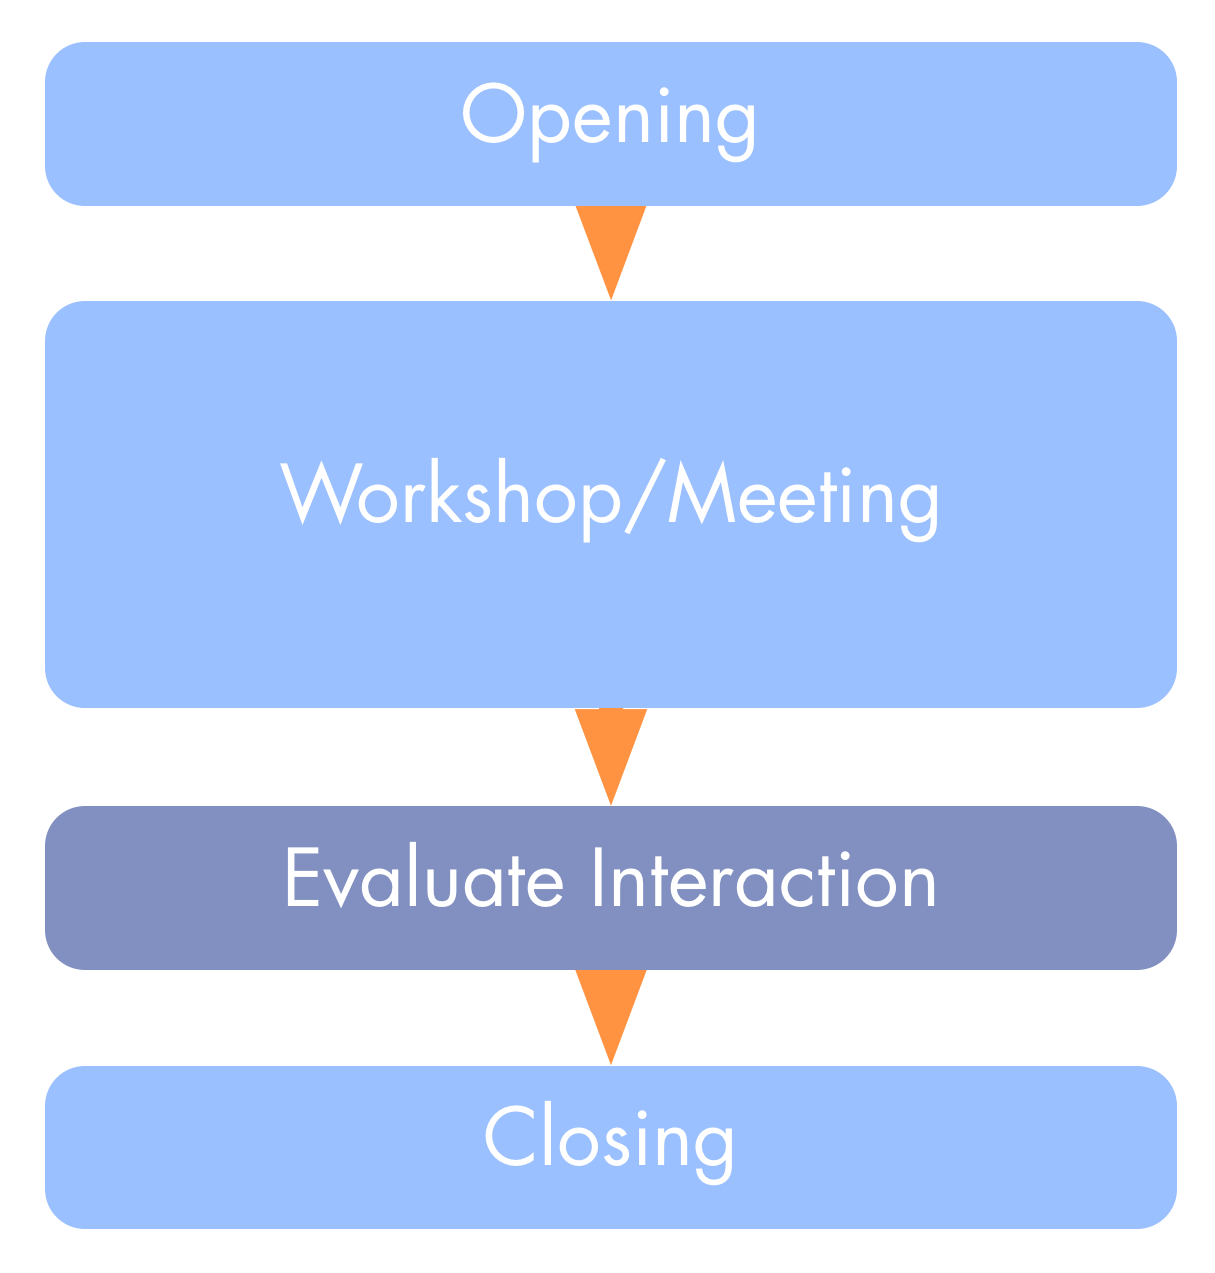
\includegraphics[keepaspectratio,width=\textwidth,height=0.75\textheight]{img/meetings/evaluate-interactions.png}
\end{figure}

\section{Meeting Facilitation}
\label{meetingfacilitation}

{\ldots}

\section{Meeting Host}
\label{meetinghost}

{\ldots}

\section{Rounds}
\label{rounds}

A group facilitation technique to maintain equivalence.

\begin{enumerate}
\item Pick a random person to start

\begin{itemize}
\item begin with a different person each time to maintain equivalence

\end{itemize}

\item Go around the circle, give everyone the chance to speak

\end{enumerate}

There's a number of ways that experienced groups can fast track certain rounds.

\begin{figure}[htbp]
\centering
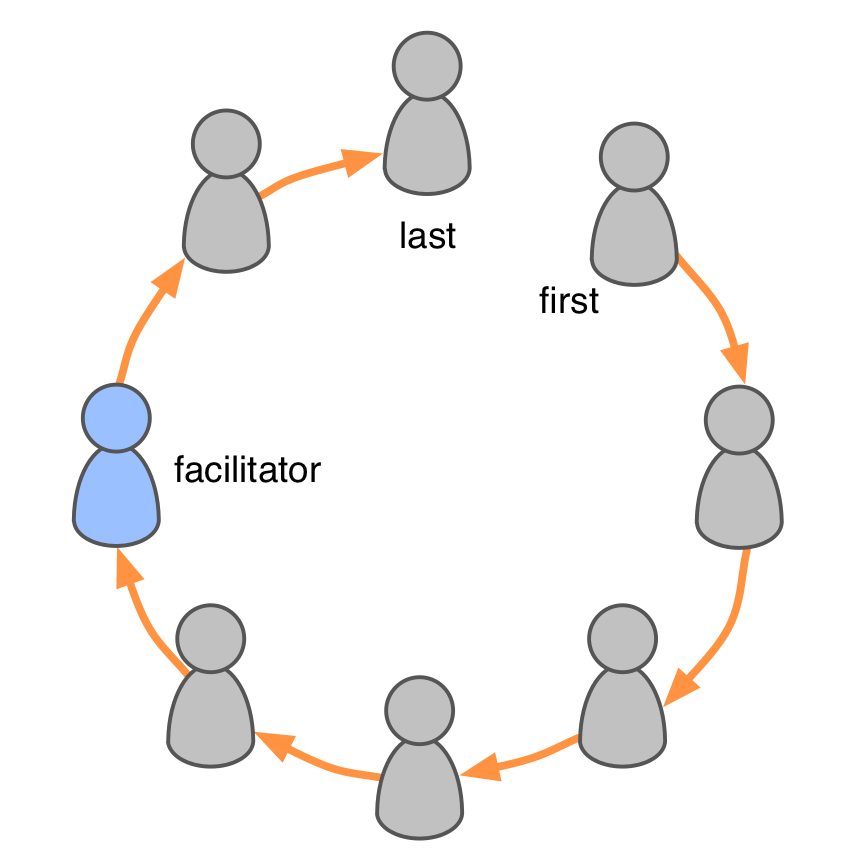
\includegraphics[keepaspectratio,width=\textwidth,height=0.75\textheight]{img/circle/rounds.png}
\end{figure}

\chapter{Coordinating Work}
\label{coordinatingwork}

{\ldots}

\section{Coordination Meeting}
\label{coordinationmeeting}

{\ldots}

\section{Coordinator Role}
\label{coordinatorrole}

{\ldots}

\section{Daily Standup}
\label{dailystandup}

\textbf{Speed up learning and improvement.}

\begin{itemize}
\item \ensuremath{\sim}15 min

\item every day at the same time

\item circle gathers around the task board

\item coordination of daily work

\item adaptation of existing agreements or creation of new agreements on the spot

\end{itemize}

\section{Planning And Review Meetings}
\label{planningandreviewmeetings}

{\ldots}

\section{Prioritized Backlog}
\label{prioritizedbacklog}

{\ldots}

\section{Pull-System For Work}
\label{pull-systemforwork}

{\ldots}

\section{Retrospective}
\label{retrospective}

\textbf{Reflect on a longer period of work and improve agreements.}

\begin{itemize}
\item \ensuremath{\sim}60 min

\item cadence, usually 2--4 weeks

\item helps seeing the bigger picture, and identifying more complex types of waste

\item What can we learn from the last iteration of work?

\item Are our tools still sharp enough?

\item Are we still going in the right direction?

\end{itemize}

\textbf{Building in continuous improvement of process:}

\begin{itemize}
\item goal: reflection on the past to guide process improvement

\item output: proposals for agreements, tensions, drivers or tasks

\item facilitated meeting (\ensuremath{\sim}1hr)

\item regular intervals (1--4 weeks)

\item adapt to situation and context:

\begin{itemize}
\item 5 phases with many different patterns for each phase

\end{itemize}

\end{itemize}

\subsection{A time to reflect on process improvement}
\label{atimetoreflectonprocessimprovement}

\begin{figure}[htbp]
\centering
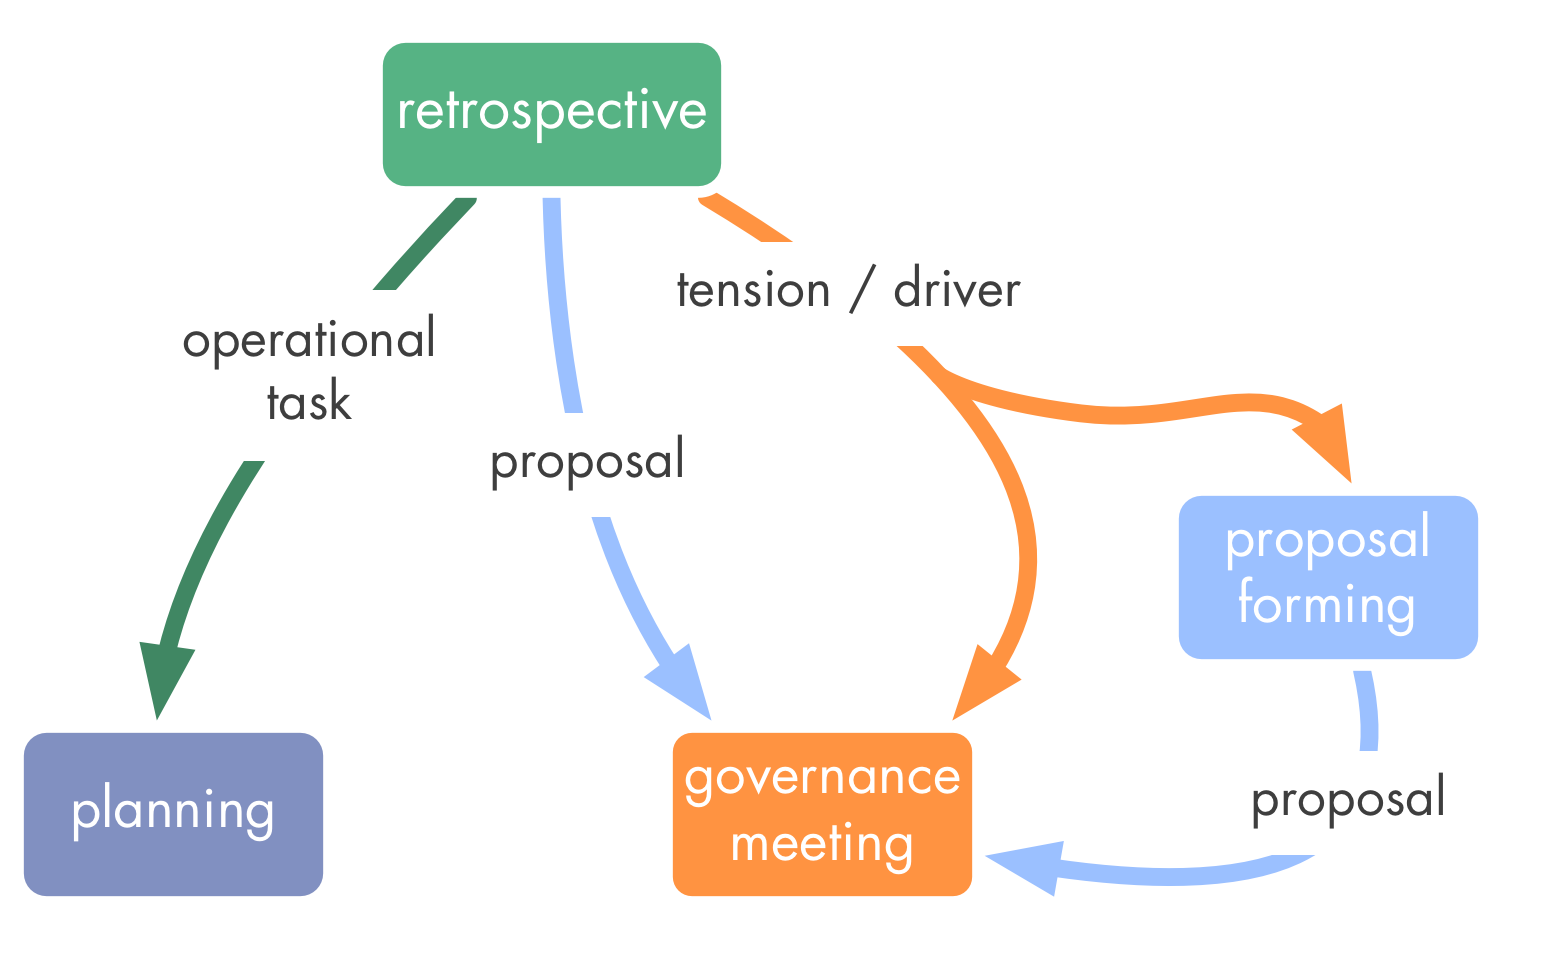
\includegraphics[keepaspectratio,width=\textwidth,height=0.75\textheight]{img/meetings/retrospective.png}
\end{figure}

\subsection{5 Phases of a Retrospective Meeting}
\label{5phasesofaretrospectivemeeting}

\begin{enumerate}
\item Set the Stage

\item Gather Data

\item Generate Insights

\item Decide What to Do

\item Close the Retrospective

\end{enumerate}

Activities for each phase can be found at \href{http://www.plans-for-retrospectives.com/}{plans-for-retrospectives.com}\footnote{\href{http://www.plans-for-retrospectives.com/}{http:/\slash www.plans-for-retrospectives.com\slash }}

\section{Visualize Work}
\label{visualizework}

{\ldots}

\chapter{Building Organizations}
\label{buildingorganizations}

{\ldots}

\section{Align Flow}
\label{alignflow}

\subsection{Flow of Value}
\label{flowofvalue}

\begin{itemize}
\item flow of value is guided by agreements (explicit and implicit), and assumptions

\item work in progress is considered waste as it ties up resources

\item continuous flow of value prevents accumulation of waste

\begin{itemize}
\item it also makes for shorter feedback loops and amplifies learning

\end{itemize}

\end{itemize}

\subsection{Flow of Value and Flow of Information}
\label{flowofvalueandflowofinformation}

\begin{figure}[htbp]
\centering
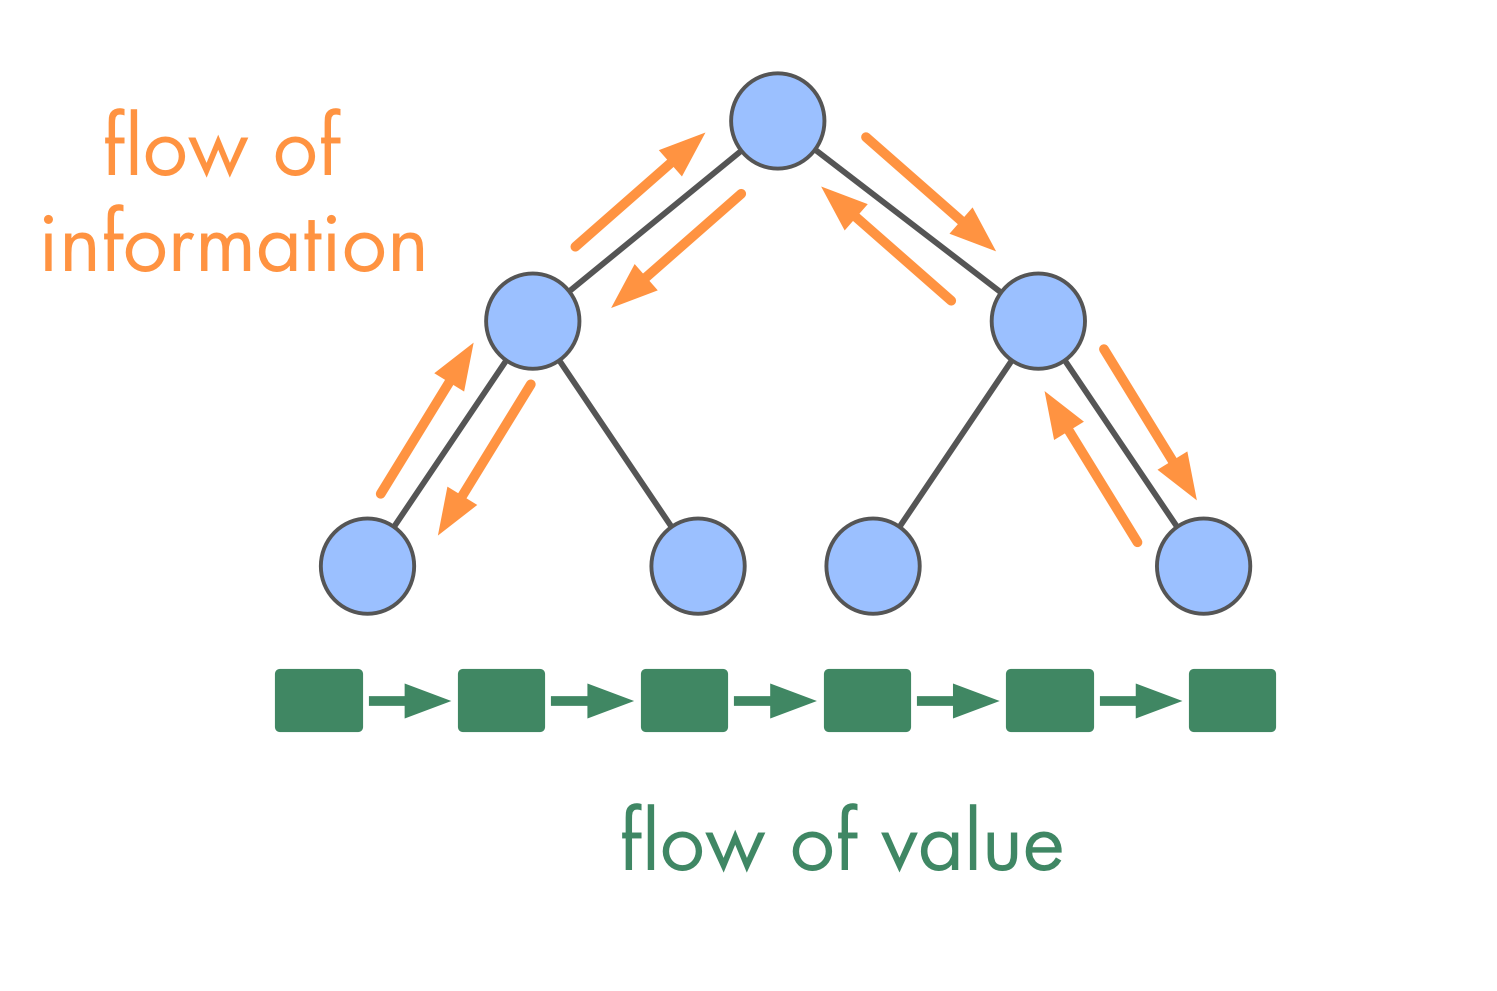
\includegraphics[keepaspectratio,width=\textwidth,height=0.75\textheight]{img/workflow-and-value/types-of-flow.png}
\end{figure}

\begin{itemize}
\item in an effective organization, the \textbf{flow of information and influence supports the continuous flow of value}

\item alignment is achieved and maintained through continuous improvement of agreements

\end{itemize}

\section{Open Systems}
\label{opensystems}

{\ldots}

\section{Organize in nested domains}
\label{organizeinnesteddomains}

{\ldots}

\chapter{People and Roles}
\label{peopleandroles}

\begin{figure}[htbp]
\centering
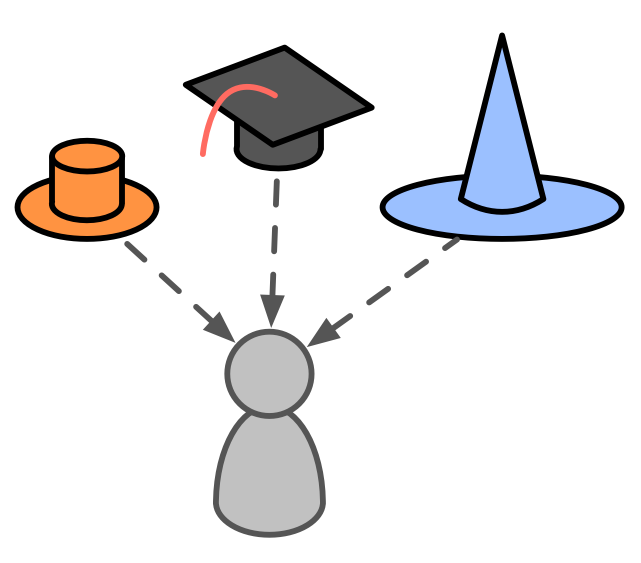
\includegraphics[keepaspectratio,width=\textwidth,height=0.75\textheight]{img/people-and-roles/roles.png}
\end{figure}

\section{People, Functions and Roles}
\label{peoplefunctionsandroles}

\begin{itemize}
\item identify functions required to respond to a driver

\item if a function is best addressed by a role:

\begin{itemize}
\item define the role

\item select people for the role

\item support development of people in the role

\end{itemize}

\end{itemize}

\section{Role Definition and Improvement}
\label{roledefinitionandimprovement}

\begin{figure}[htbp]
\centering
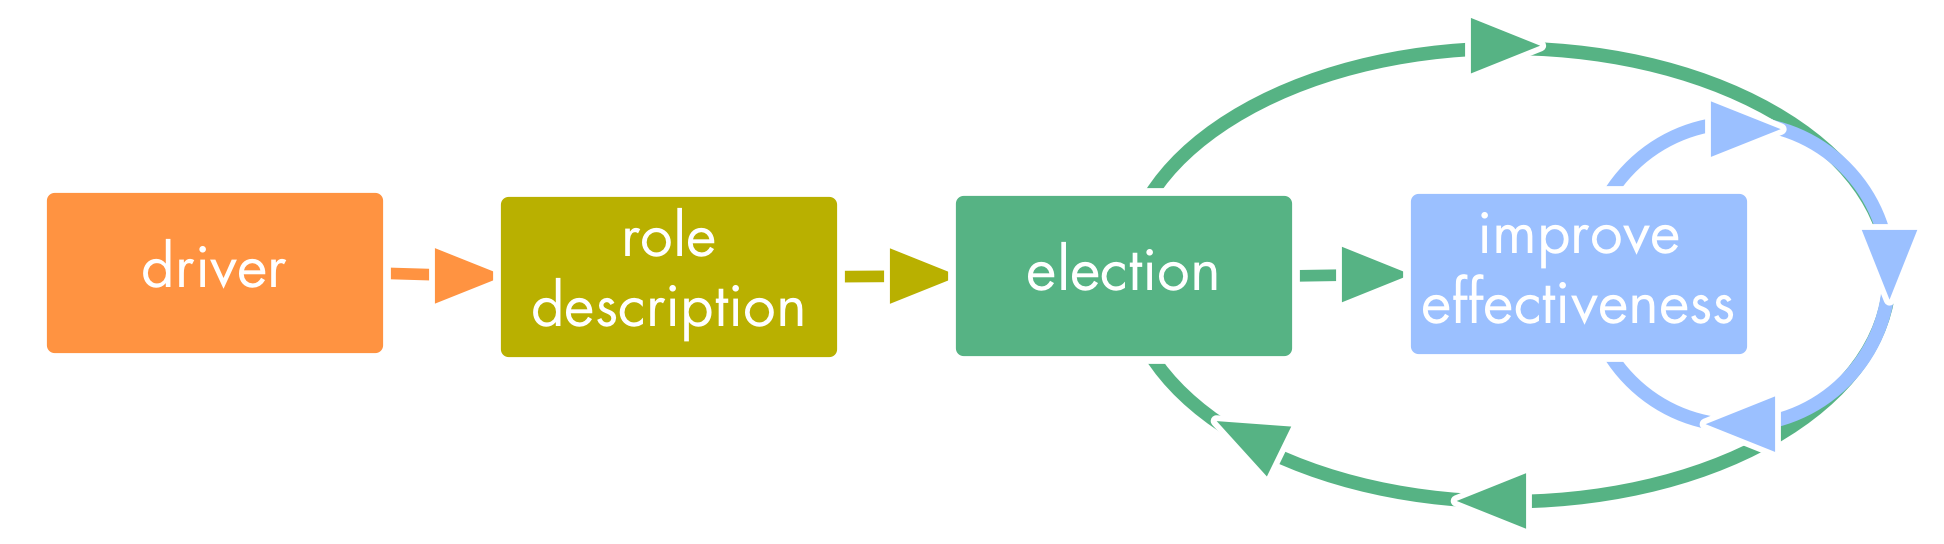
\includegraphics[keepaspectratio,width=\textwidth,height=0.75\textheight]{img/people-and-roles/role-improvement.png}
\end{figure}

\section{Performance Improvement Process}
\label{performanceimprovementprocess}

Continuous improvement of the effectiveness of people in roles \#\#

\begin{enumerate}
\item Conduct effectiveness review

\item Create development plan

\item Full circle consents to development plan

\item Act on the plan

\end{enumerate}

\begin{figure}[htbp]
\centering
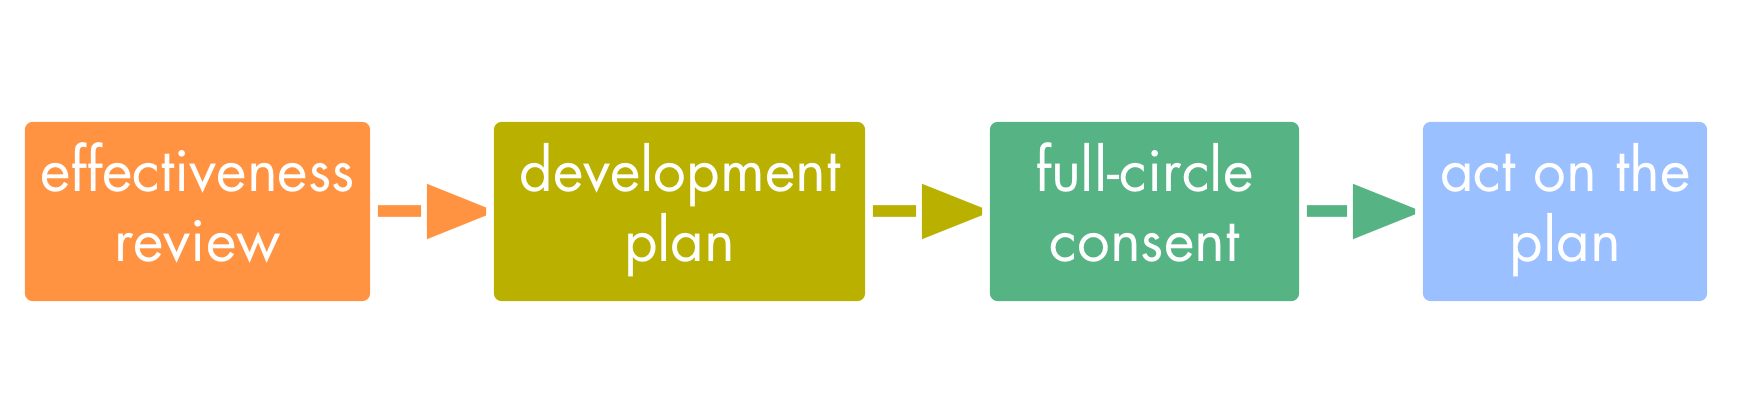
\includegraphics[keepaspectratio,width=\textwidth,height=0.75\textheight]{img/people-and-roles/performance-improvement-process.png}
\end{figure}

{\ldots}

\section{Development Plan}
\label{developmentplan}

\textbf{Contents:}

\begin{itemize}
\item current role description

\item appreciations

\item areas for improvement

\item action items to improve effectiveness

\item evaluation criteria

\item suggested amendments to role description

\end{itemize}

\section{Effectiveness Review}
\label{effectivenessreview}

\begin{itemize}
\item a process to harvest appreciations, identify opportunities for improvement and evolve the role

\item the individual holding the role initiates the process and begins each step

\end{itemize}

\subsection{Steps}
\label{steps}

\begin{enumerate}
\item Invite people with complementing perspectives to contribute to the review, and a facilitator

\item Collect appreciations

\item Identify areas for improvement

\begin{itemize}
\item personal development

\item updates to role description, function or driver

\end{itemize}

\item Co-create and consent to a development plan

\end{enumerate}

\begin{figure}[htbp]
\centering
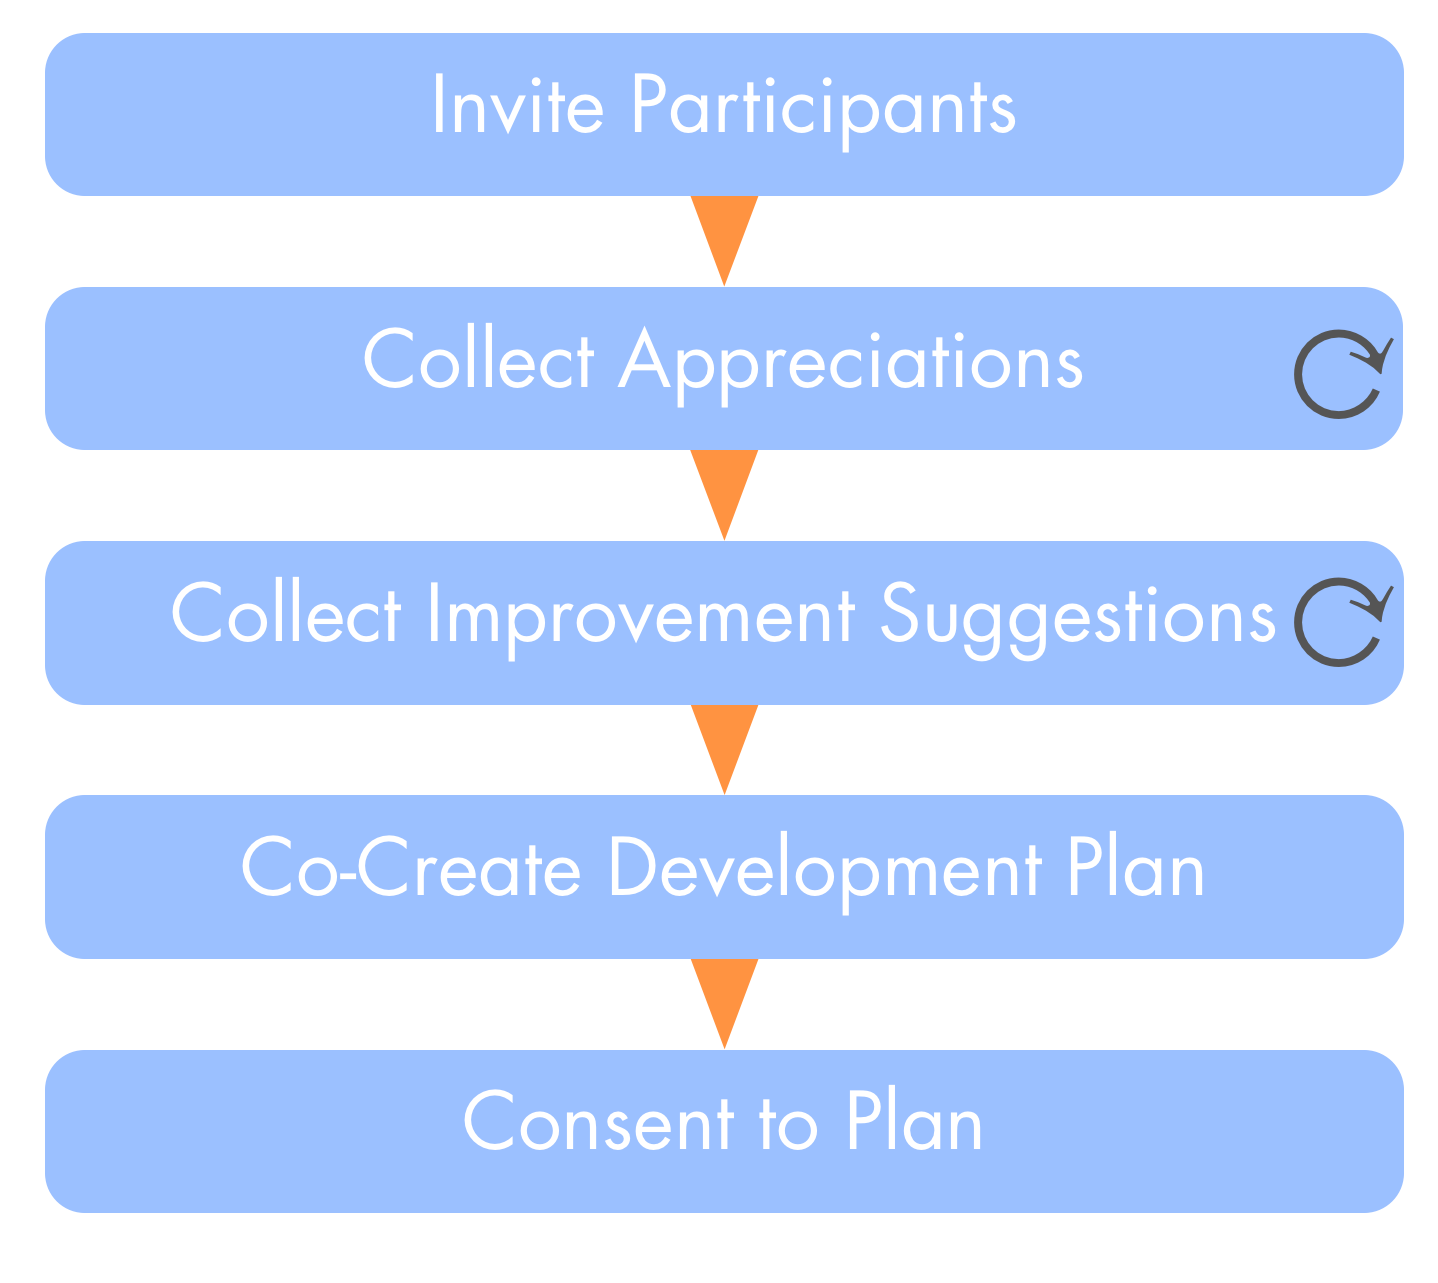
\includegraphics[keepaspectratio,width=\textwidth,height=0.75\textheight]{img/people-and-roles/effectiveness-review.png}
\end{figure}

\section{Role}
\label{role}

{\ldots}

\section{Role Description}
\label{roledescription}

\begin{itemize}
\item role descriptions can be created using proposal forming

\item a minimal role description contains:

\begin{itemize}
\item driver

\item term

\item key responsibilities

\item preferable skills, experience and qualities

\item cadence of effectiveness reviews

\end{itemize}

\end{itemize}

\subsection{Template for Role Descriptions}
\label{templateforroledescriptions}

\begin{figure}[htbp]
\centering
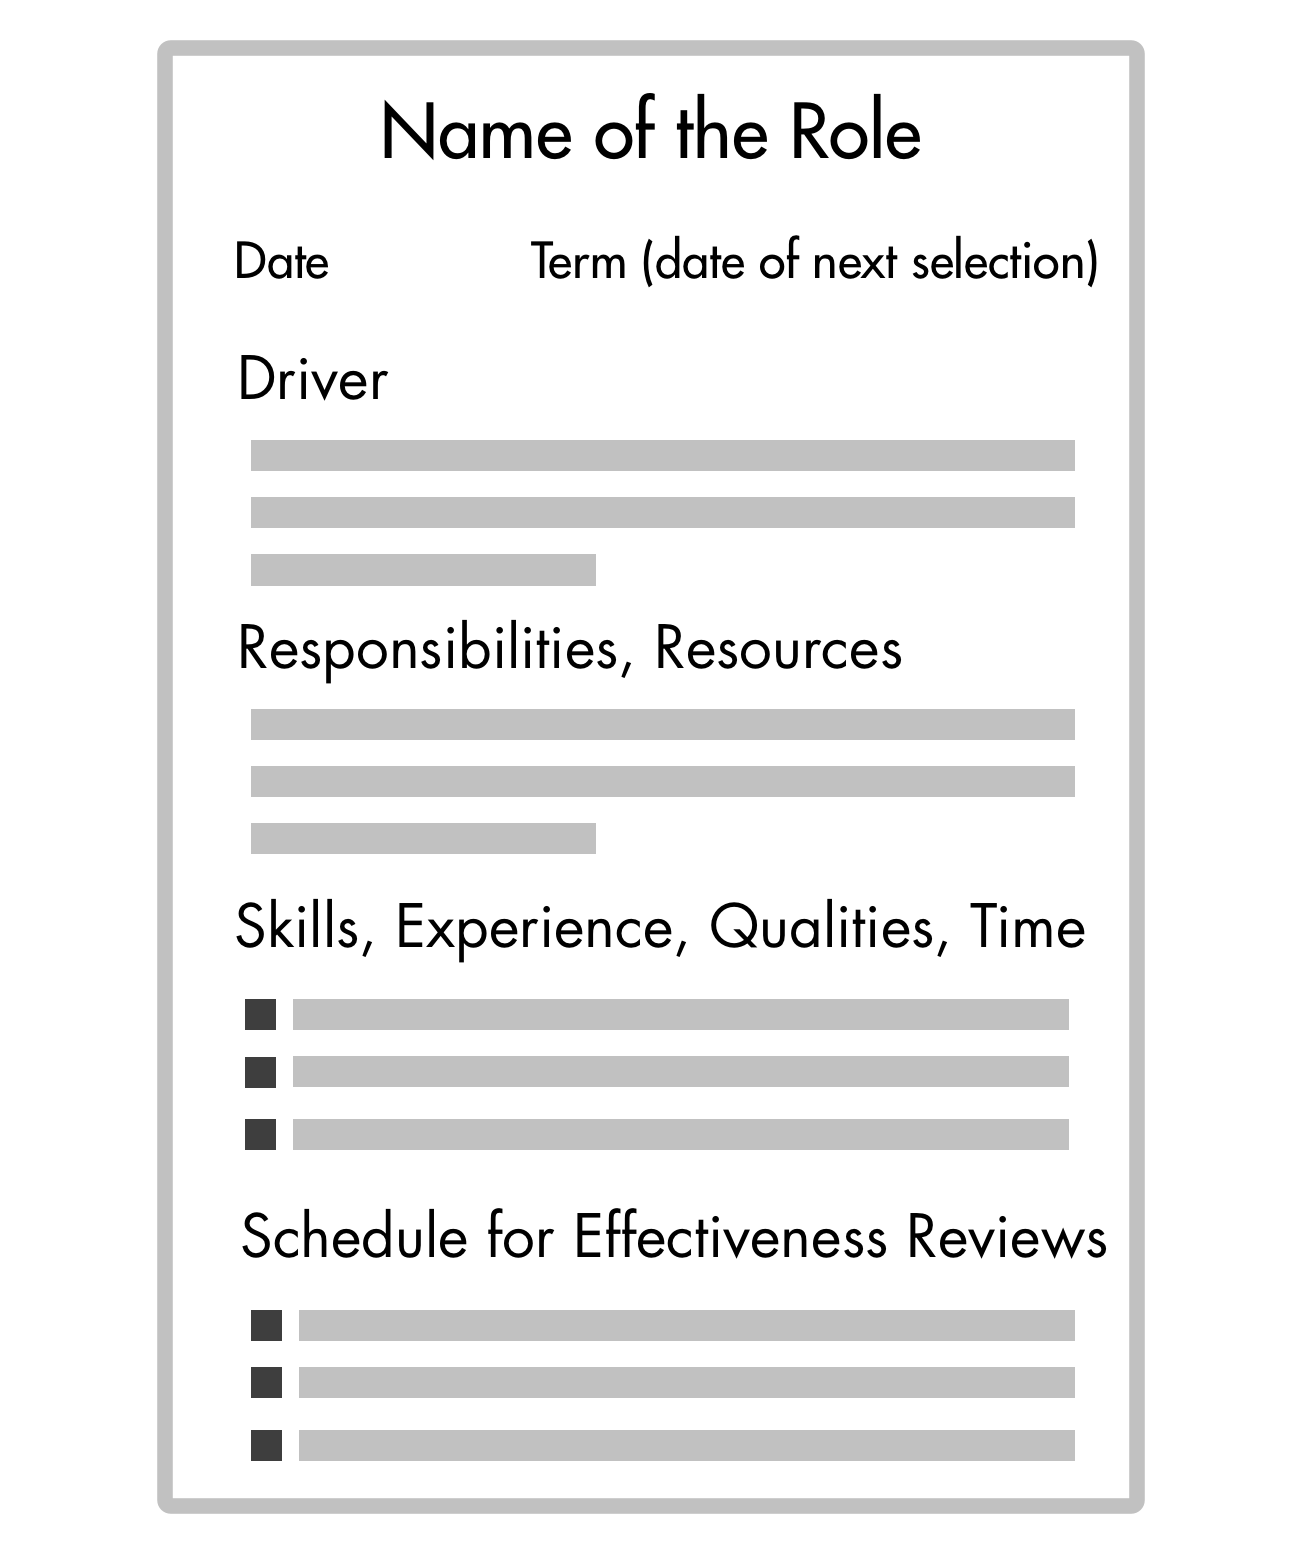
\includegraphics[keepaspectratio,width=\textwidth,height=0.75\textheight]{img/people-and-roles/role-description-template.png}
\end{figure}

\section{Role Selection}
\label{roleselection}

\begin{figure}[htbp]
\centering
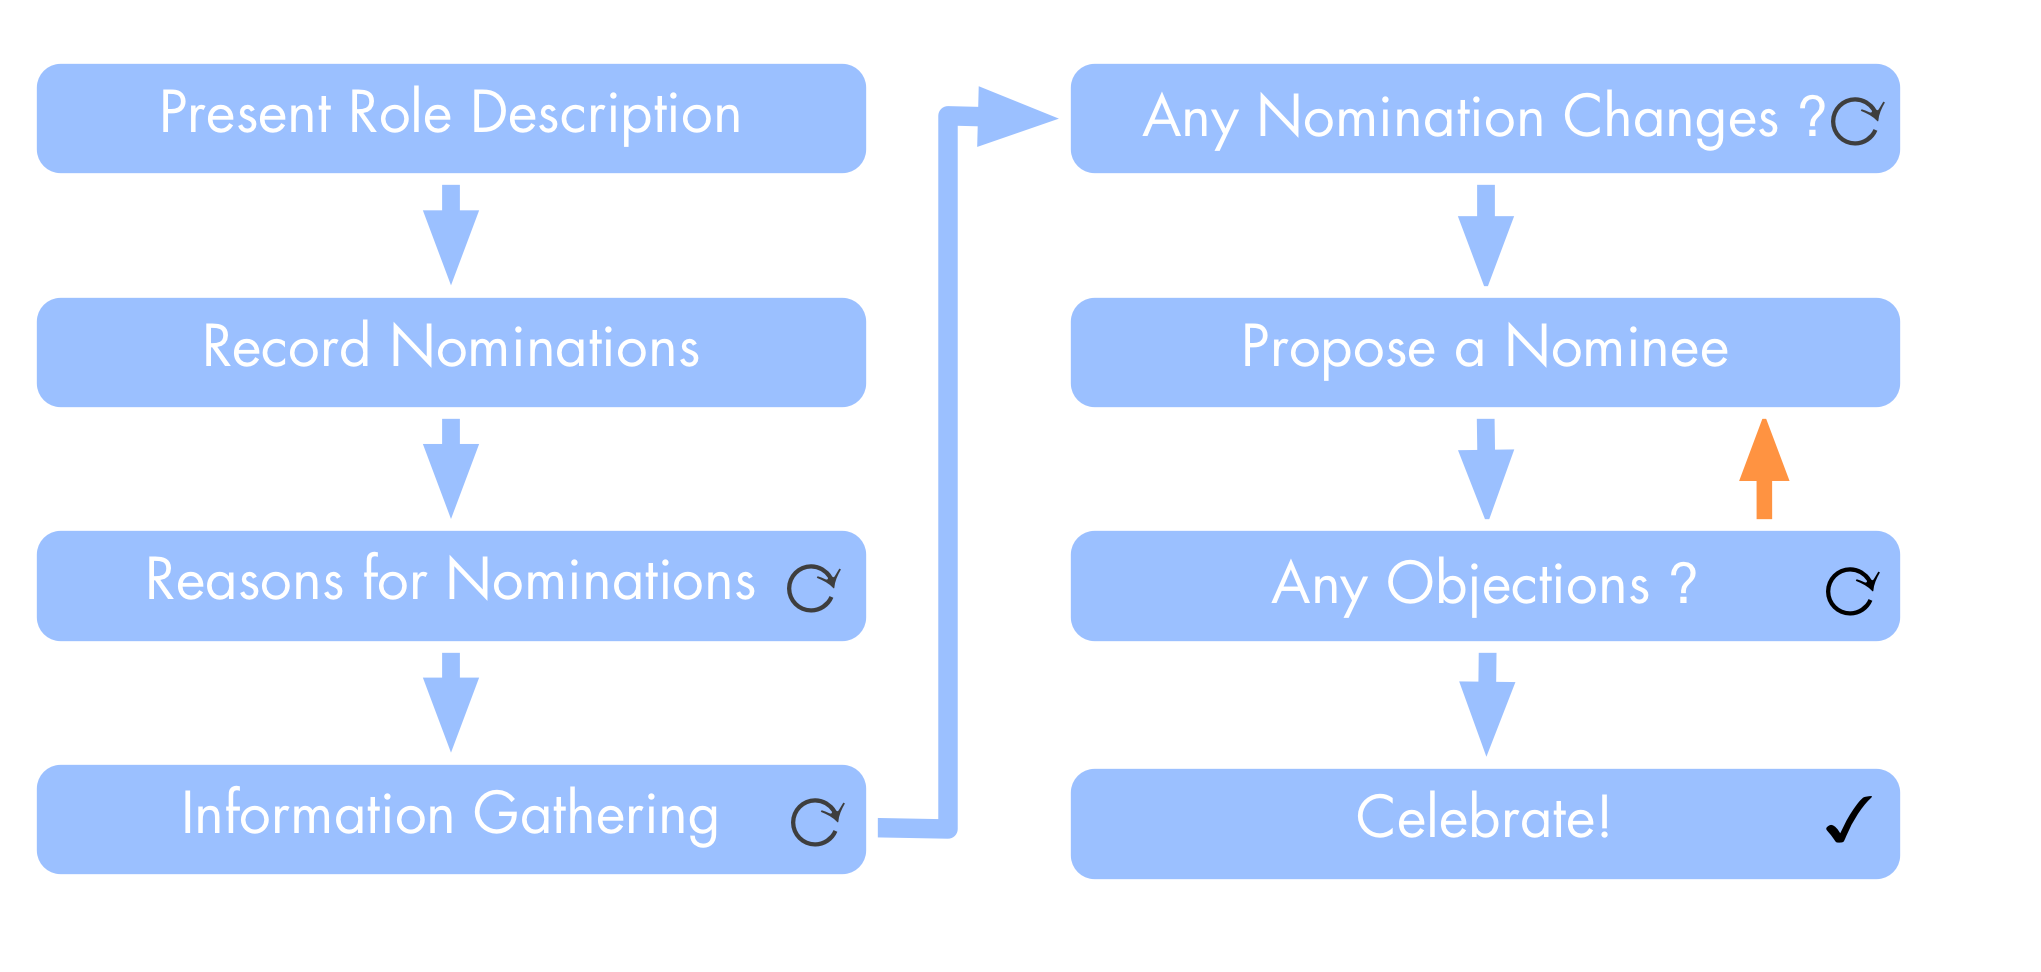
\includegraphics[keepaspectratio,width=\textwidth,height=0.75\textheight]{img/people-and-roles/selection.png}
\end{figure}

\begin{itemize}
\item People avoid expressing interest before elections

\item Nominations are made on the strength of the reason

\begin{itemize}
\item not according to the majority

\end{itemize}

\item You can nominate yourself or pass

\item When harvesting objections, ask the candidate last

\item Objections may be resolved by amending the role description or by nominating someone else

\end{itemize}

\section{Support Roles}
\label{supportroles}

{\ldots}

\chapter{Organizational Structure}
\label{organizationalstructure}

The primary function of organizational structure is \textbf{to enable effective collaboration} by aligning the flow of information to support the flow of value..

\textbf{Organizational structure needs to evolve continuously} in order to adapt to a changing environment.

\textbf{Semi-autonomous, self-organizing and self-governing circles} are the basic building blocks for organizational structure.

\section{Structural Patterns}
\label{structuralpatterns}

\begin{itemize}
\item Sociocracy 3.0 describes a variety of patterns to grow organizational structure

\item patterns apply to different layers of abstraction (basic, micro, macro and meta)

\item different patterns serve different drivers

\item patterns can be combined as needed

\item more patterns are out there and will be discovered

\end{itemize}

\section{Backbone Organization}
\label{backboneorganization}

A pattern for multi-stakeholder projects or services.

\begin{figure}[htbp]
\centering
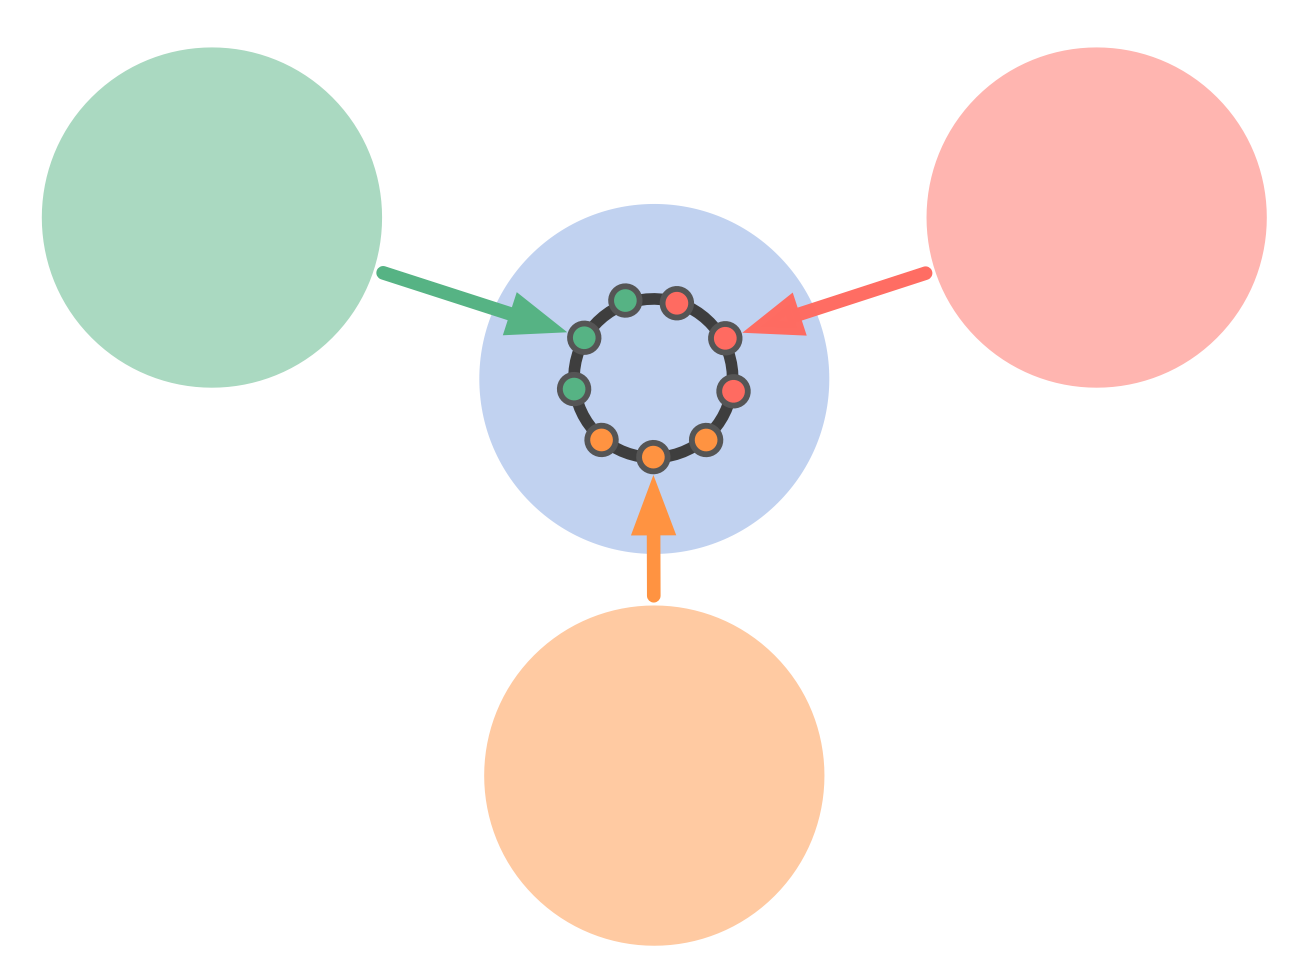
\includegraphics[keepaspectratio,width=\textwidth,height=0.75\textheight]{img/structural-patterns/backbone-organization.png}
\end{figure}

\section{Coordination Circle}
\label{coordinationcircle}

{\ldots}

\section{Delegate Circle}
\label{delegatecircle}

A pattern for coordination

\begin{figure}[htbp]
\centering
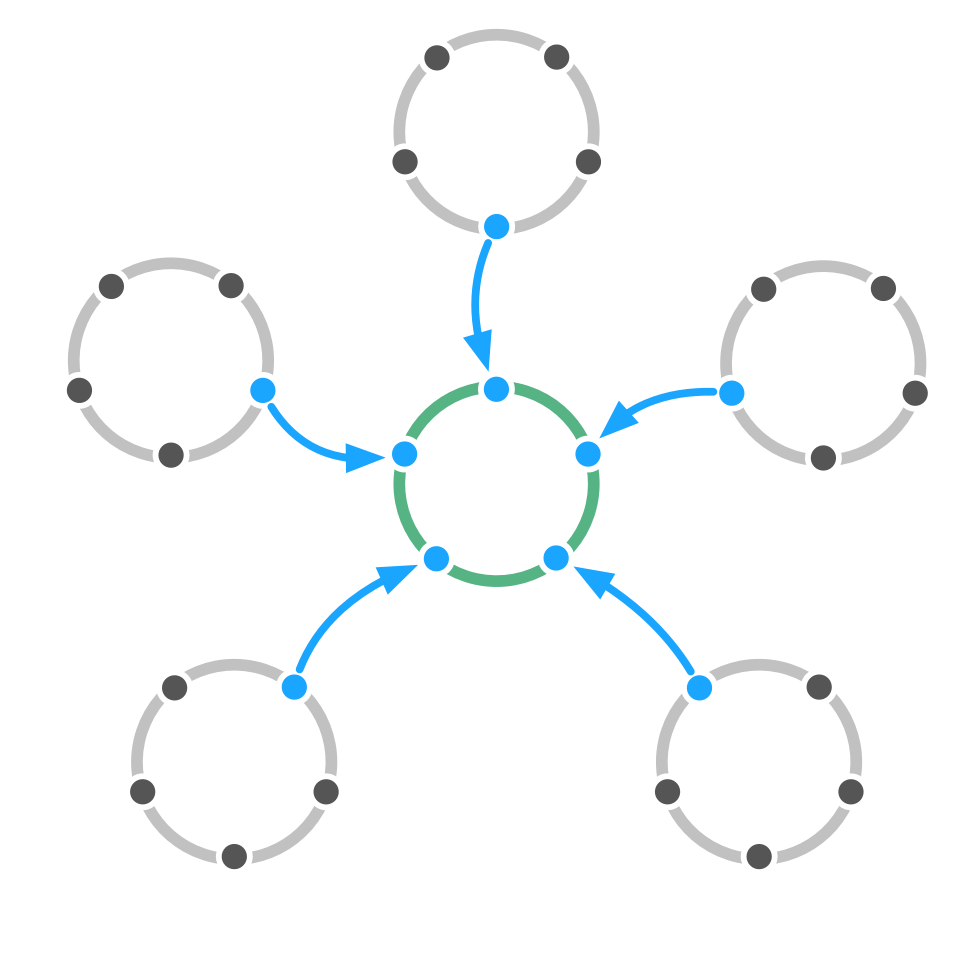
\includegraphics[keepaspectratio,width=\textwidth,height=0.75\textheight]{img/structural-patterns/delegate-circle.png}
\end{figure}

\section{Double Linking}
\label{doublelinking}

\begin{figure}[htbp]
\centering
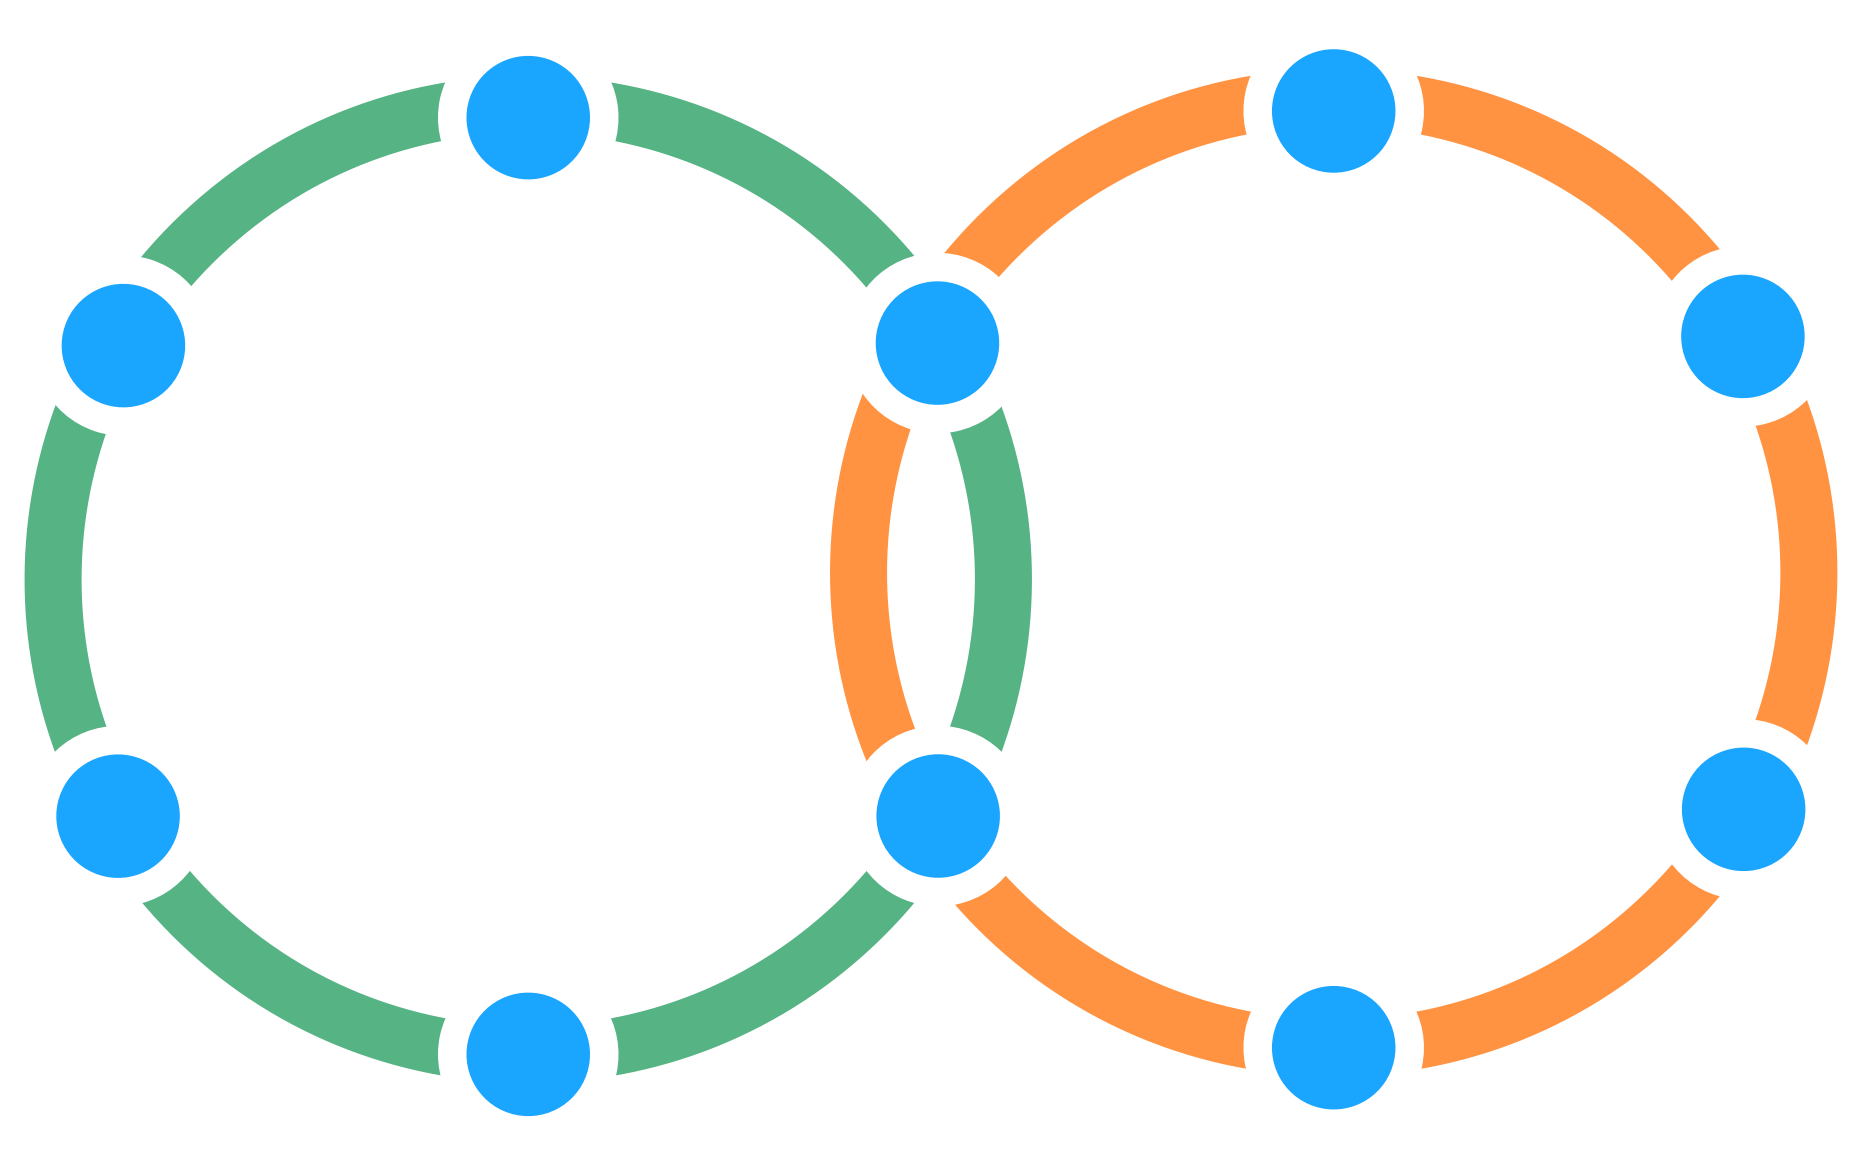
\includegraphics[keepaspectratio,width=\textwidth,height=0.75\textheight]{img/structural-patterns/double-link.png}
\end{figure}

\subsection{Facilitate two-way flow of information and influence}
\label{facilitatetwo-wayflowofinformationandinfluence}

\begin{itemize}
\item Two interdependent circles each elect a representative to participate as full members in both circles' governance meetings

\item can be used to prevent tensions in hierarchical structures

\end{itemize}

\section{Double-Linked Hierarchy}
\label{double-linkedhierarchy}

A pattern for the early phase of a transformation \#\#

\begin{figure}[htbp]
\centering
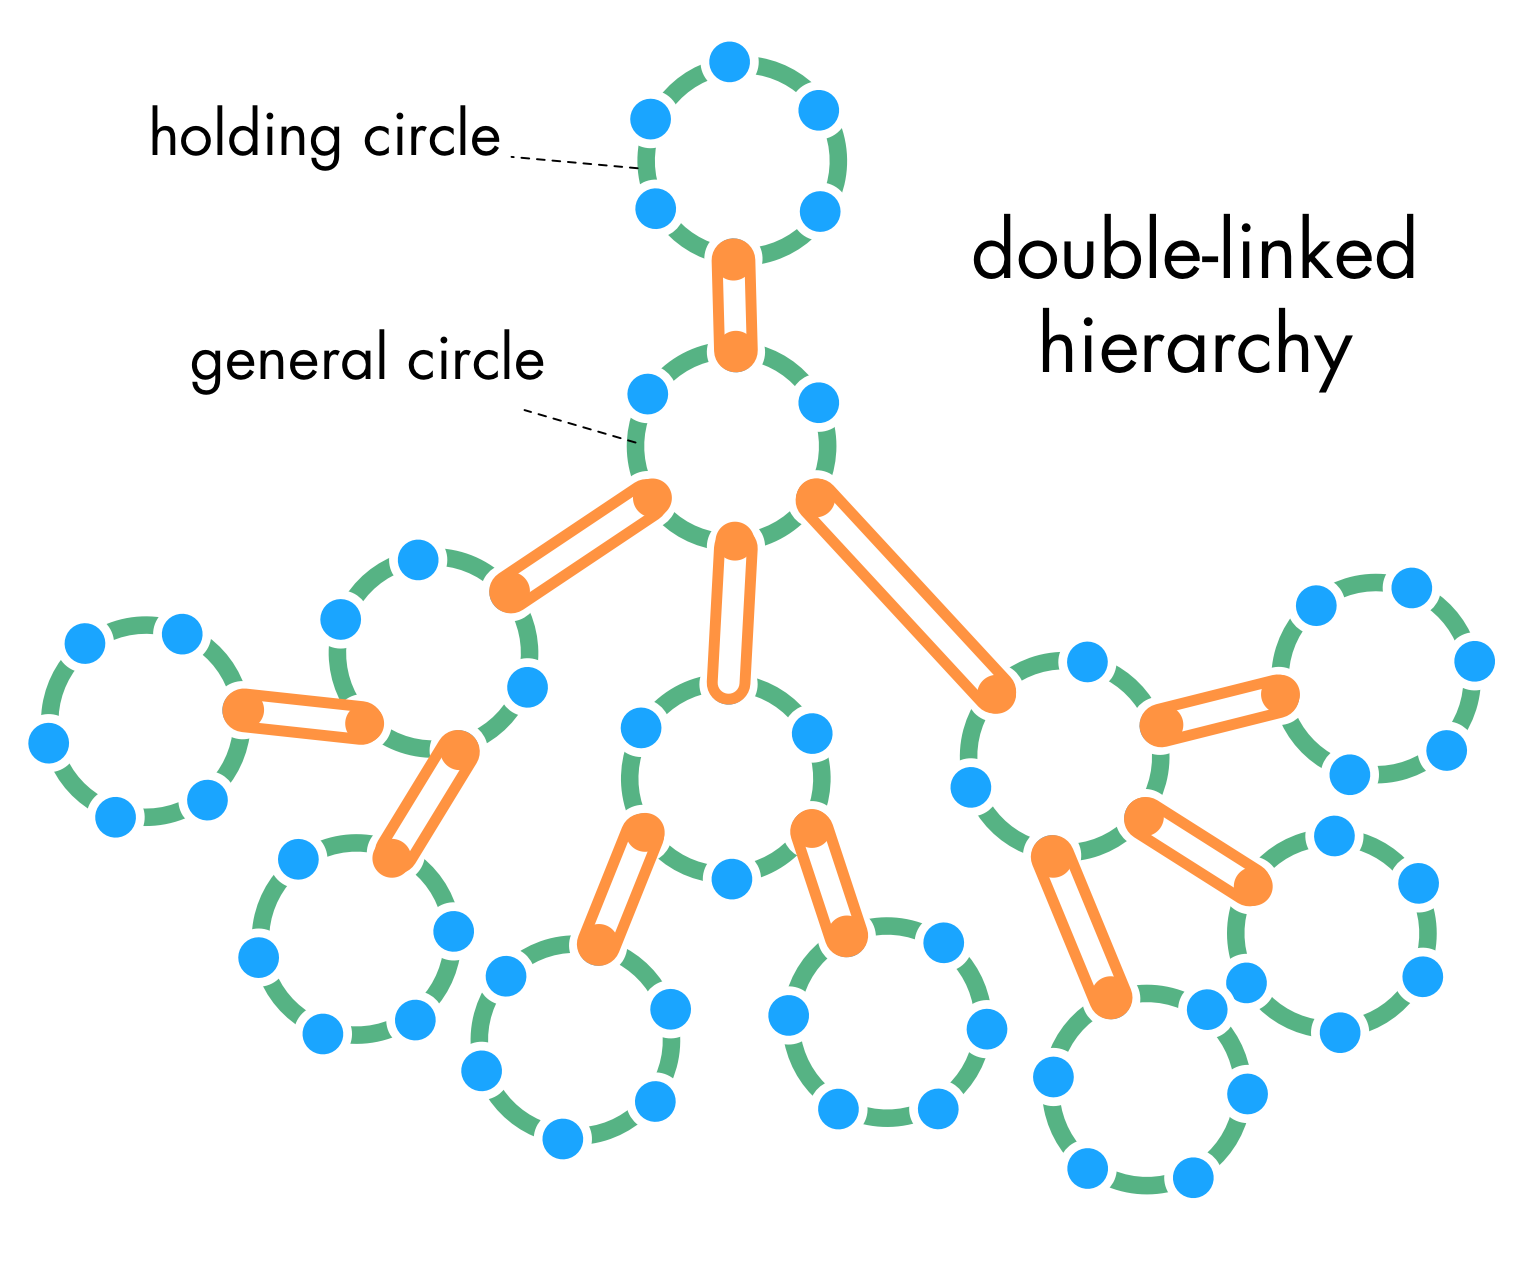
\includegraphics[keepaspectratio,width=\textwidth,height=0.75\textheight]{img/structural-patterns/double-linked-hierarchy.png}
\end{figure}

\section{Fractal Organization}
\label{fractalorganization}

A Pattern for learning, coordination and alignment across organizational boundaries.

\begin{figure}[htbp]
\centering
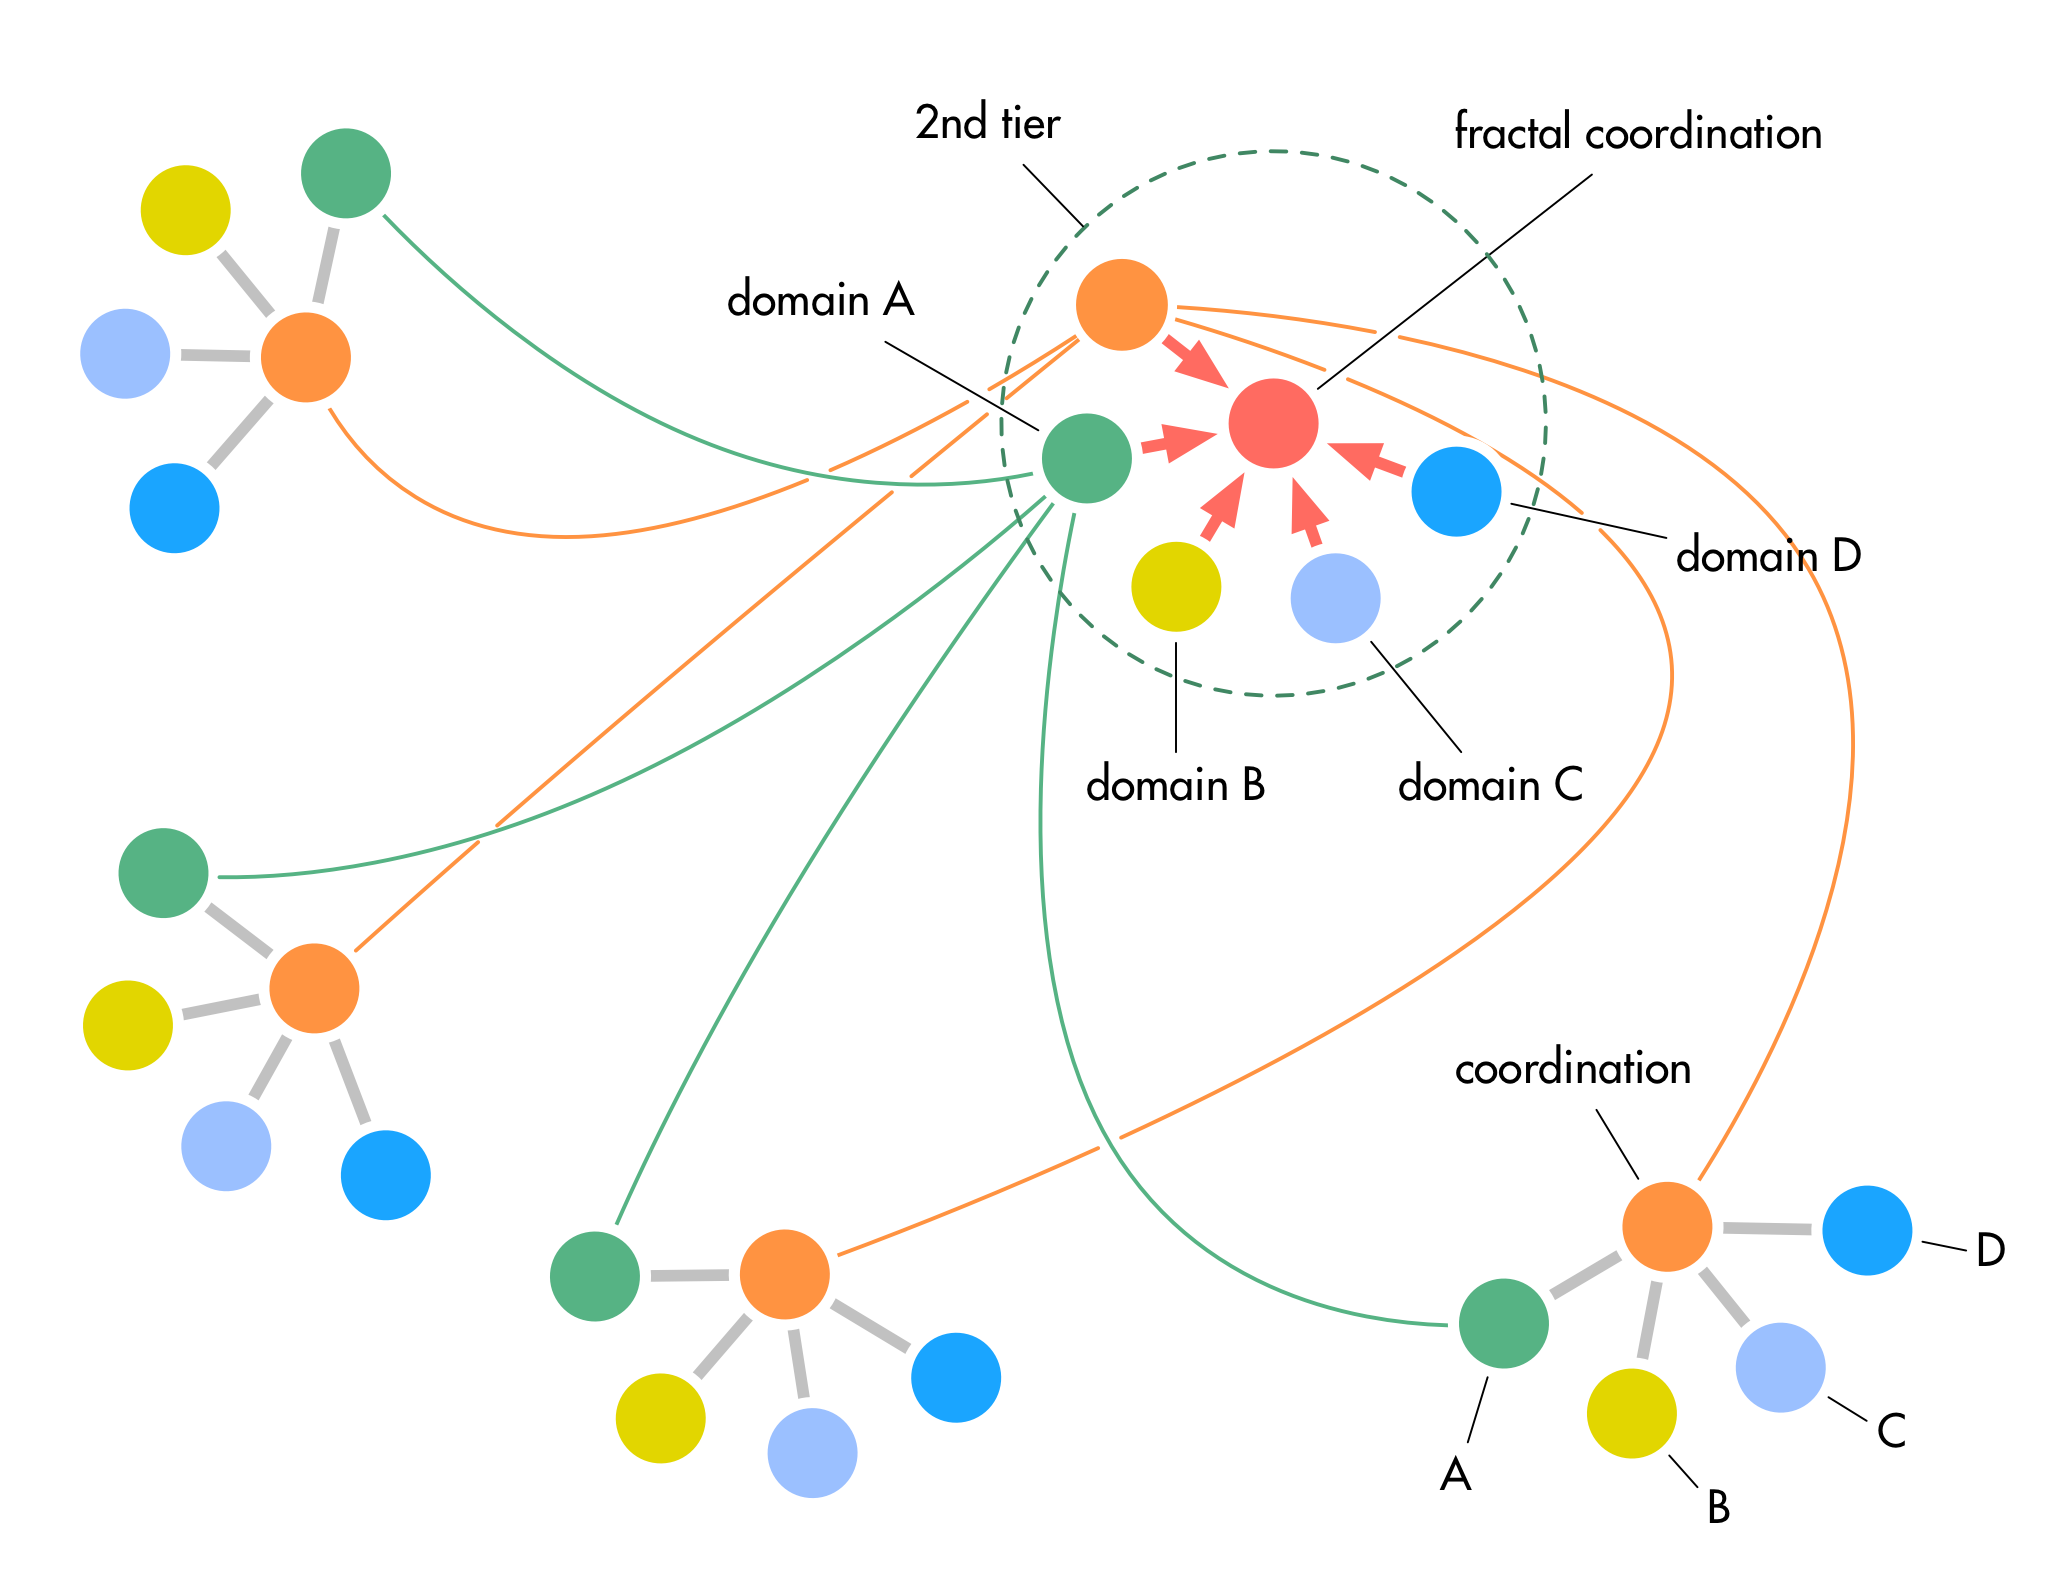
\includegraphics[keepaspectratio,width=\textwidth,height=0.75\textheight]{img/structural-patterns/fractal-organization.png}
\end{figure}

\section{Helping Circle}
\label{helpingcircle}

{\ldots}

\section{Nested Circle}
\label{nestedcircle}

A pattern for expanding functions

\begin{figure}[htbp]
\centering
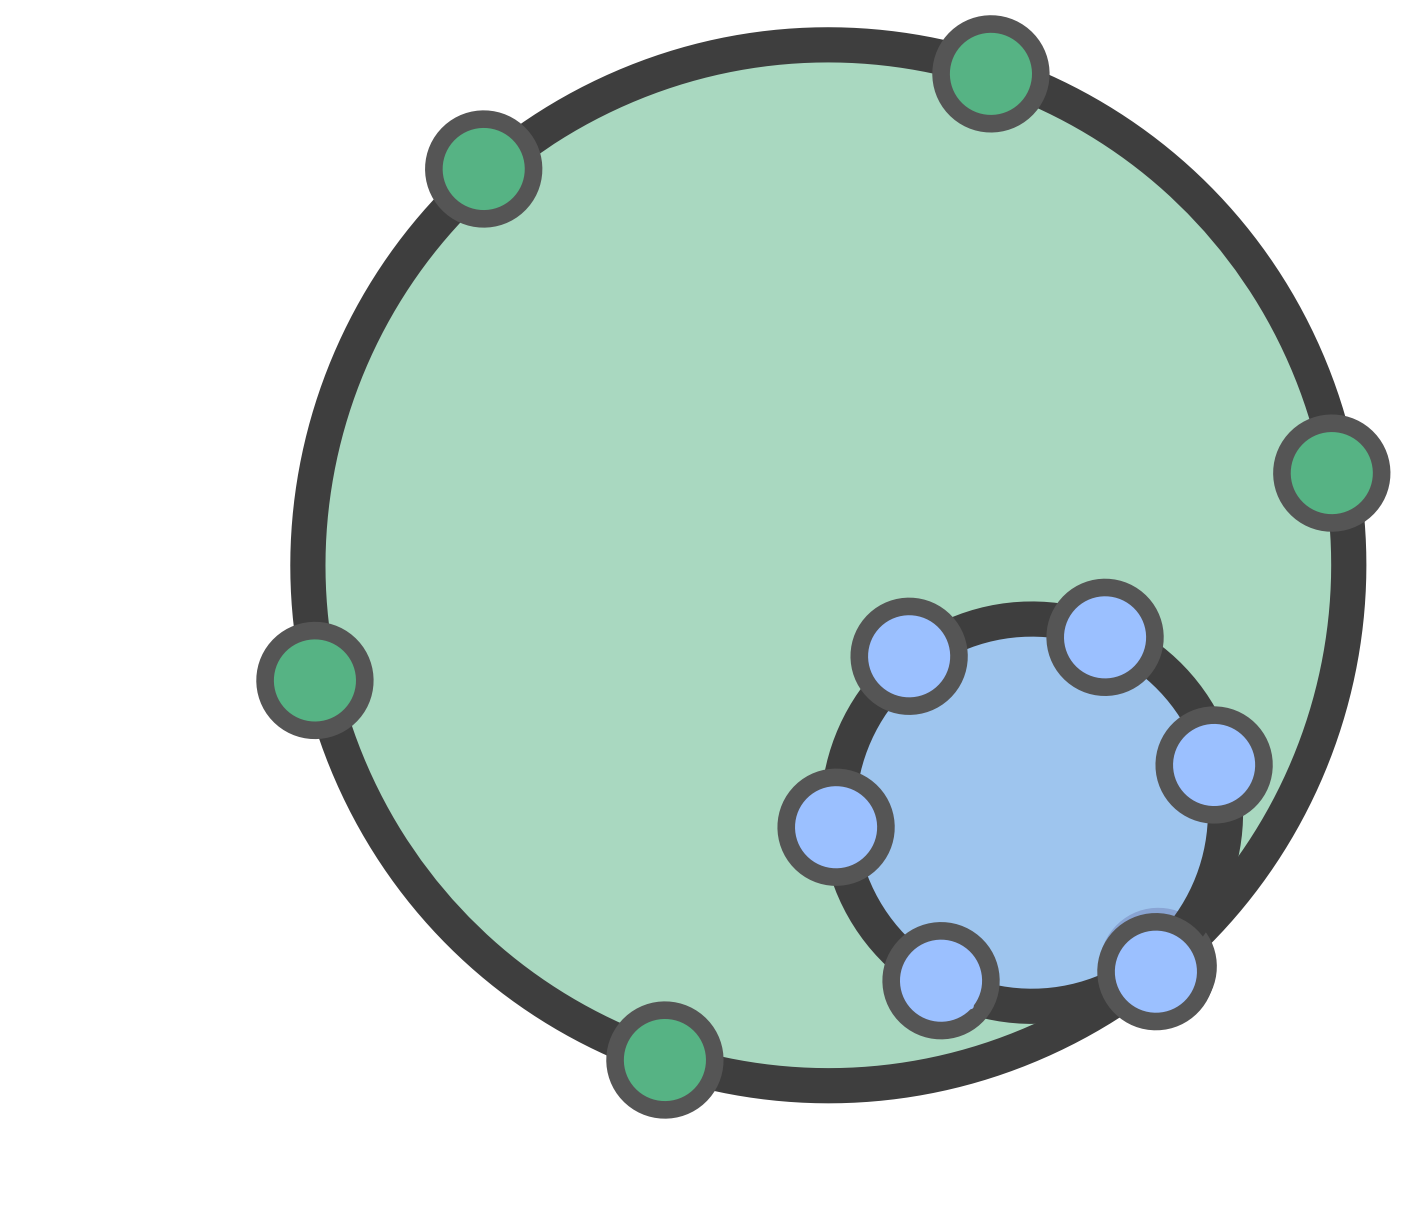
\includegraphics[keepaspectratio,width=\textwidth,height=0.75\textheight]{img/structural-patterns/nested-circle.png}
\end{figure}

\section{Peach Organization}
\label{peachorganization}

Periphery drives the organization, the center provides services.

\begin{figure}[htbp]
\centering
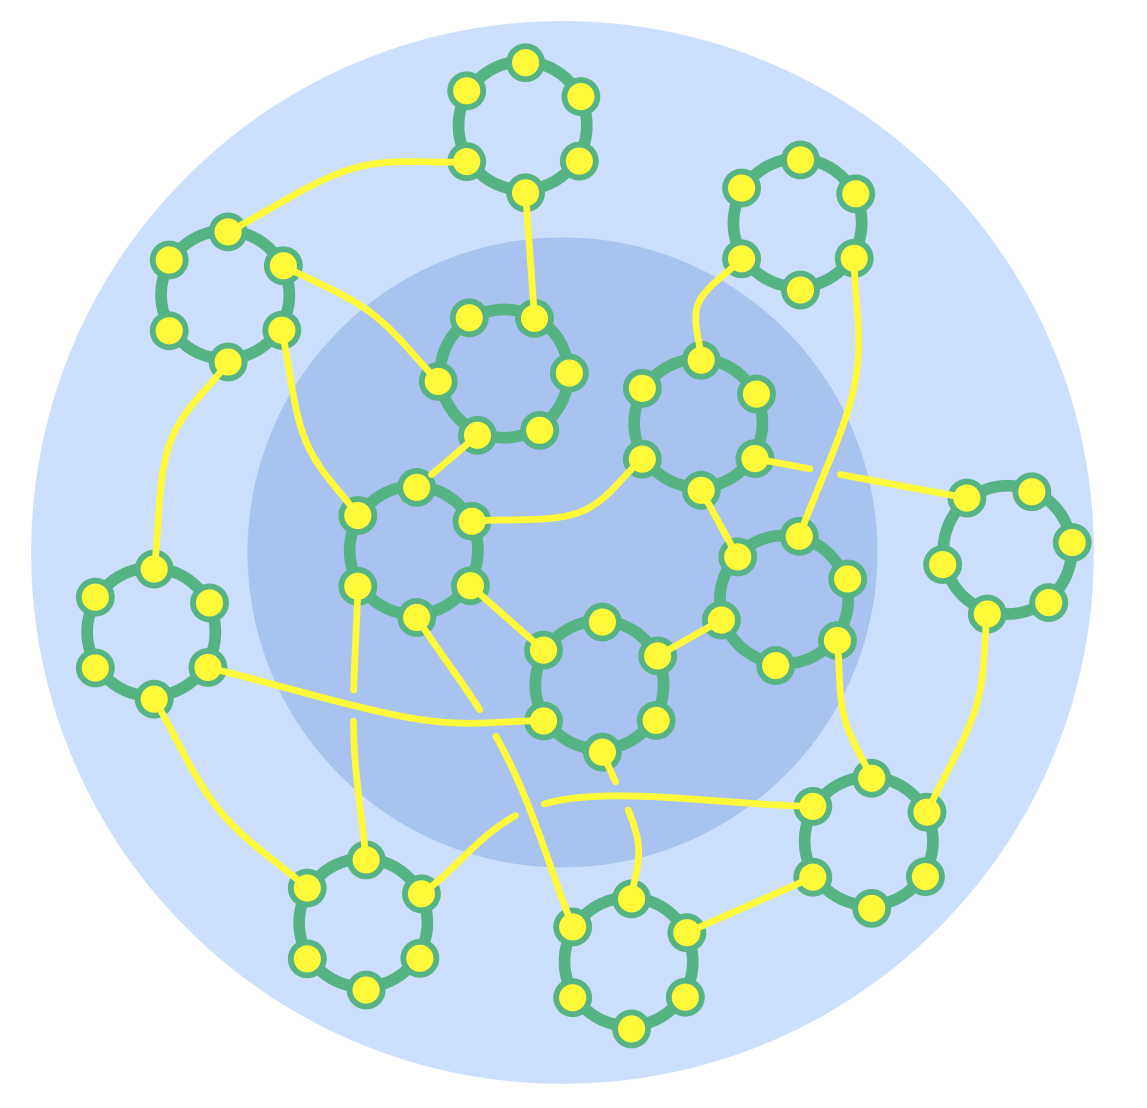
\includegraphics[keepaspectratio,width=\textwidth,height=0.75\textheight]{img/structural-patterns/peach-organization.png}
\end{figure}

\section{Representative}
\label{representative}

Representatives (a.k.a Links){\ldots}:

\begin{itemize}
\item {\ldots}stand for the interests of one circle in another circle

\item {\ldots}are elected for a limited term

\item {\ldots}participate as full members in governance meetings of the other circle and can:

\begin{itemize}
\item raise items for the agenda

\item object to agreements and proposals

\end{itemize}

\end{itemize}

\section{Service Circle}
\label{servicecircle}

A pattern for outsourcing shared services

\begin{figure}[htbp]
\centering
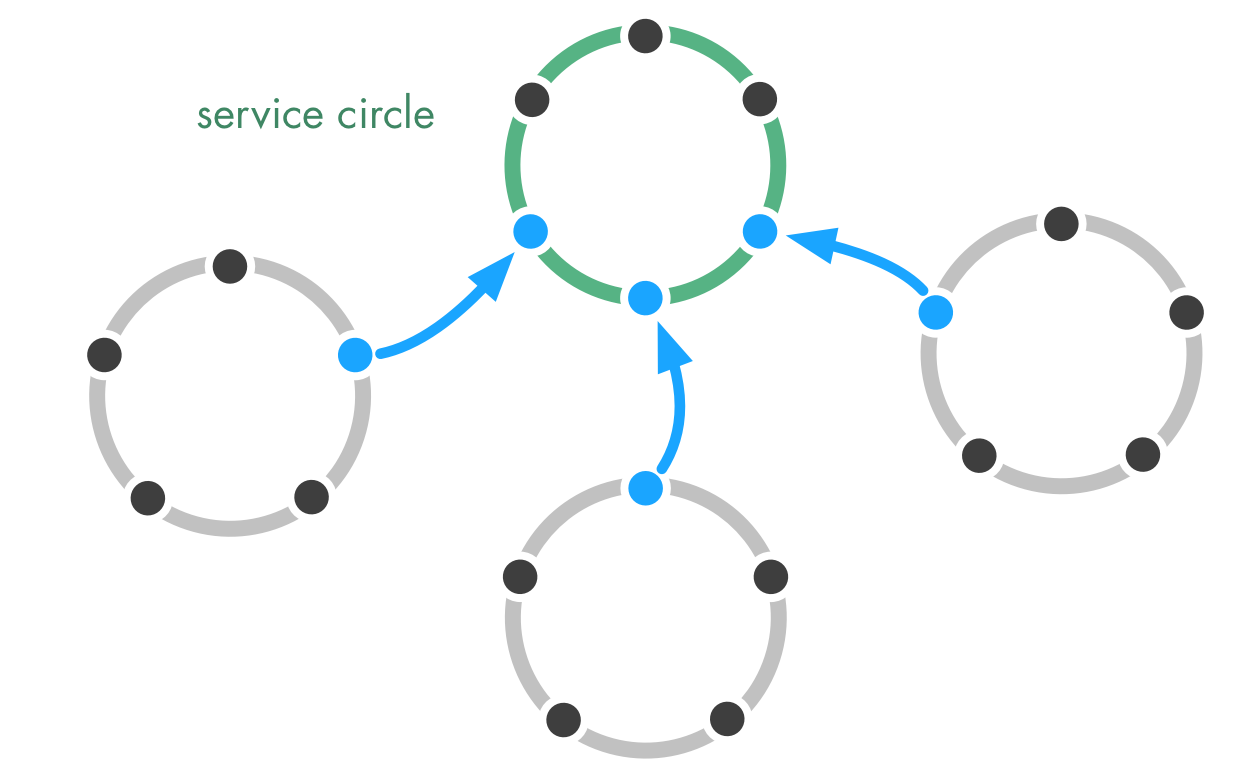
\includegraphics[keepaspectratio,width=\textwidth,height=0.75\textheight]{img/structural-patterns/service-circle.png}
\end{figure}

\chapter{Bringing In S3 Patterns}
\label{bringingins3patterns}

{\ldots}

\section{Adapt Patterns To Context}
\label{adaptpatternstocontext}

{\ldots}

\section{Be The Change}
\label{bethechange}

{\ldots}

\section{Continuous Improvement Of Work Process}
\label{continuousimprovementofworkprocess}

{\ldots}

\section{Open S3 Adoption}
\label{opens3adoption}

{\ldots}

\section{Pull-System For Organizational Change}
\label{pull-systemfororganizationalchange}

{\ldots}

\chapter{Alignment}
\label{alignment}

{\ldots}

\section{Adopt the Seven Principles}
\label{adoptthesevenprinciples}

\begin{itemize}
\item values embrace Sociocracy 3.0 principles

\item collaboration follows principles and values

\end{itemize}

\begin{figure}[htbp]
\centering
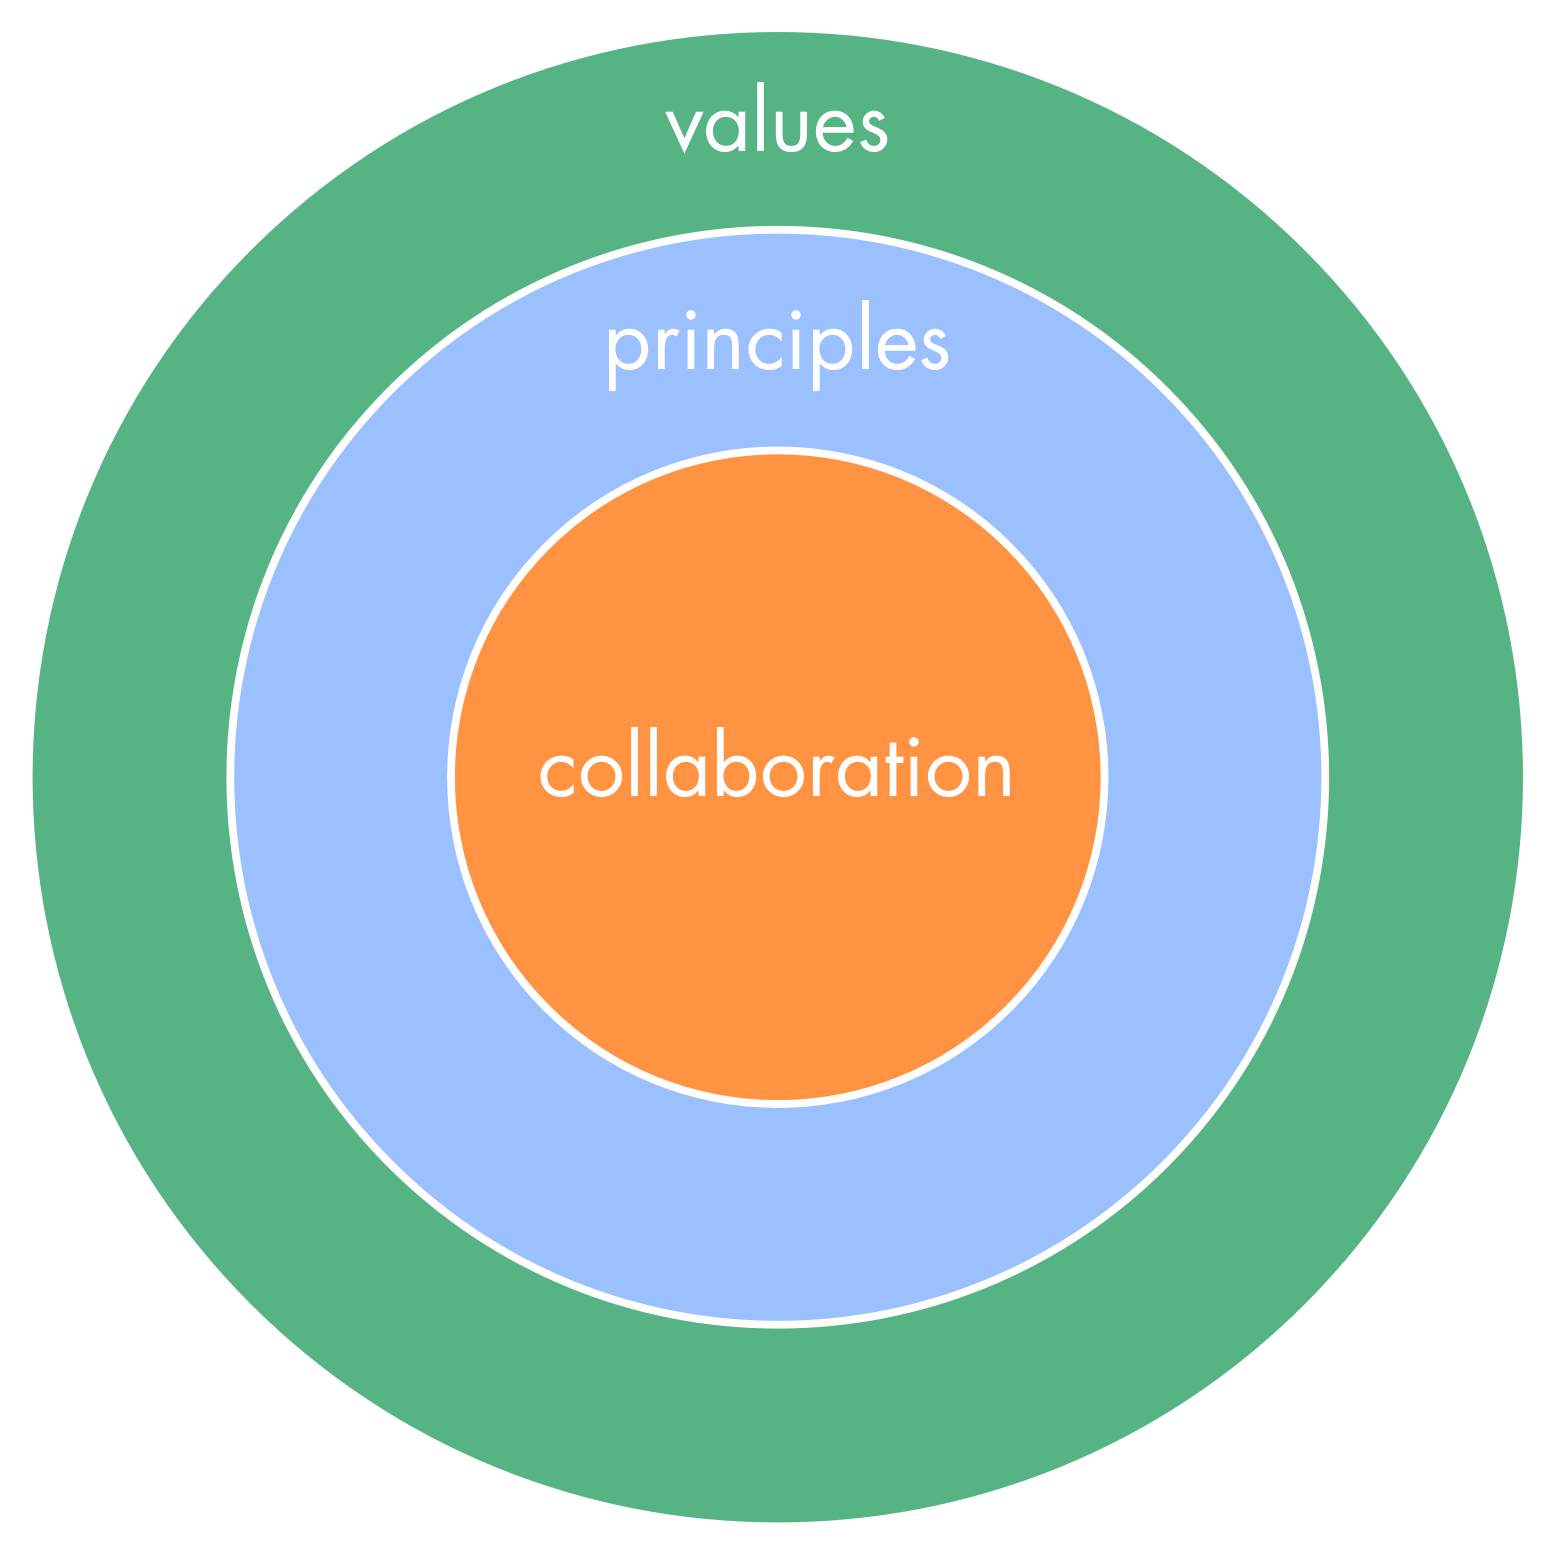
\includegraphics[keepaspectratio,width=\textwidth,height=0.75\textheight]{img/collaboration-values/values-step3.png}
\end{figure}

\section{Agree On Values}
\label{agreeonvalues}

\textbf{Definition:} \emph{A value is a principle of some significance that guides behavior.}

\begin{itemize}
\item In an organization people come together to collaborate

\item every individual has values that are influenced by their experiences and beliefs

\item values may define ethical limitations to action

\end{itemize}

\begin{figure}[htbp]
\centering
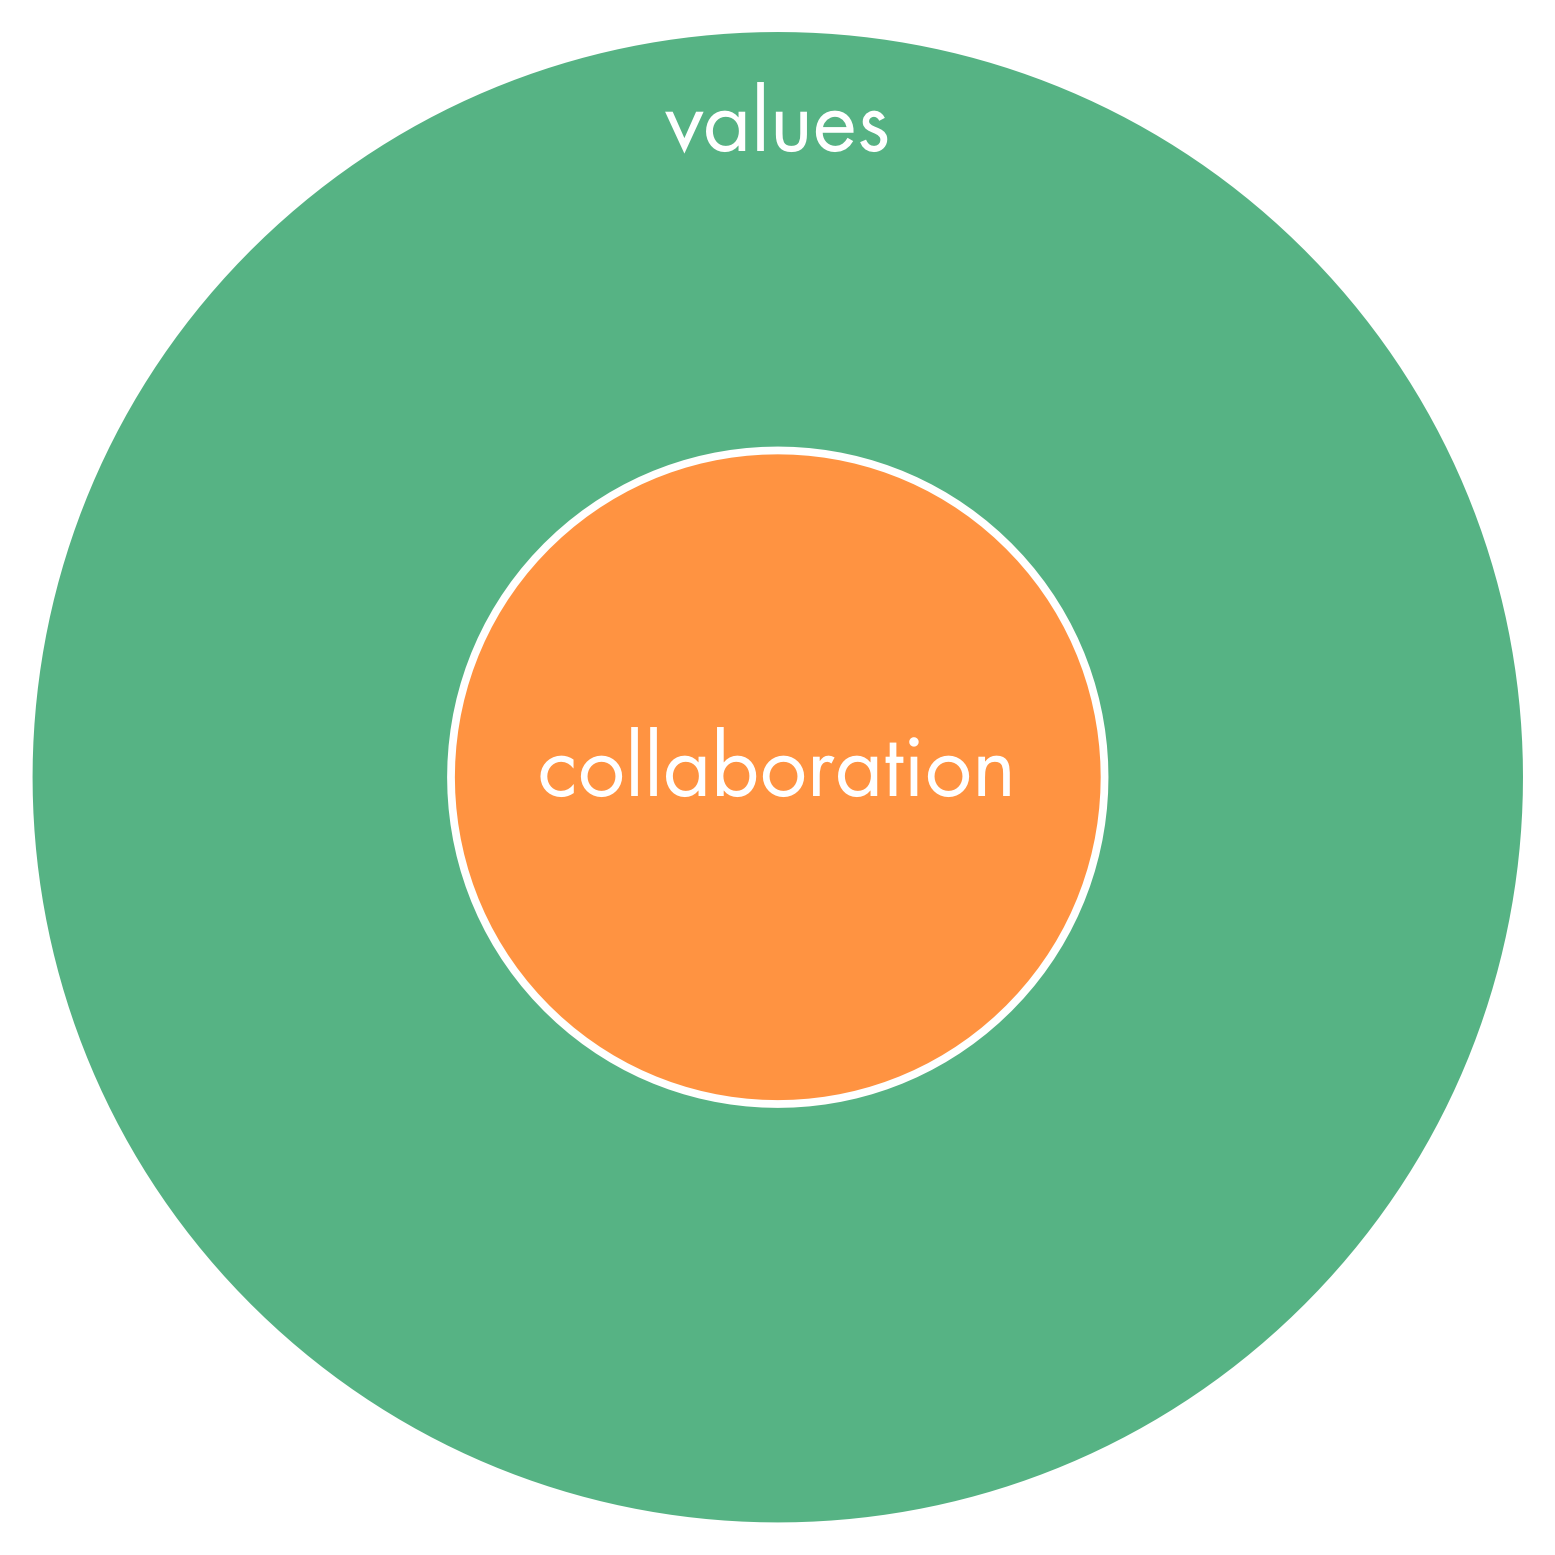
\includegraphics[keepaspectratio,width=\textwidth,height=0.75\textheight]{img/collaboration-values/values-step2.png}
\end{figure}

\begin{itemize}
\item organizational values \textbf{define culture} and set parameters for action

\item values offer guidance to determine appropriate action, even in the absence of explicit agreements

\item a group or organization may \textbf{choose to collectively adopt values}

\item defining values is a \textbf{strategy} that supports effectiveness of an organization:

\begin{itemize}
\item reduces potential for \textbf{misunderstanding}

\item \textbf{aligns} decision making and action

\item \textbf{attracts new members, partners and customers} who are aligned with the organization

\end{itemize}

\item values are an agreement, and thus subject to \textbf{regular reviews}

\end{itemize}

\section{Bylaws}
\label{bylaws}

{\ldots}

\section{Contracting And Accountability}
\label{contractingandaccountability}

\begin{figure}[htbp]
\centering
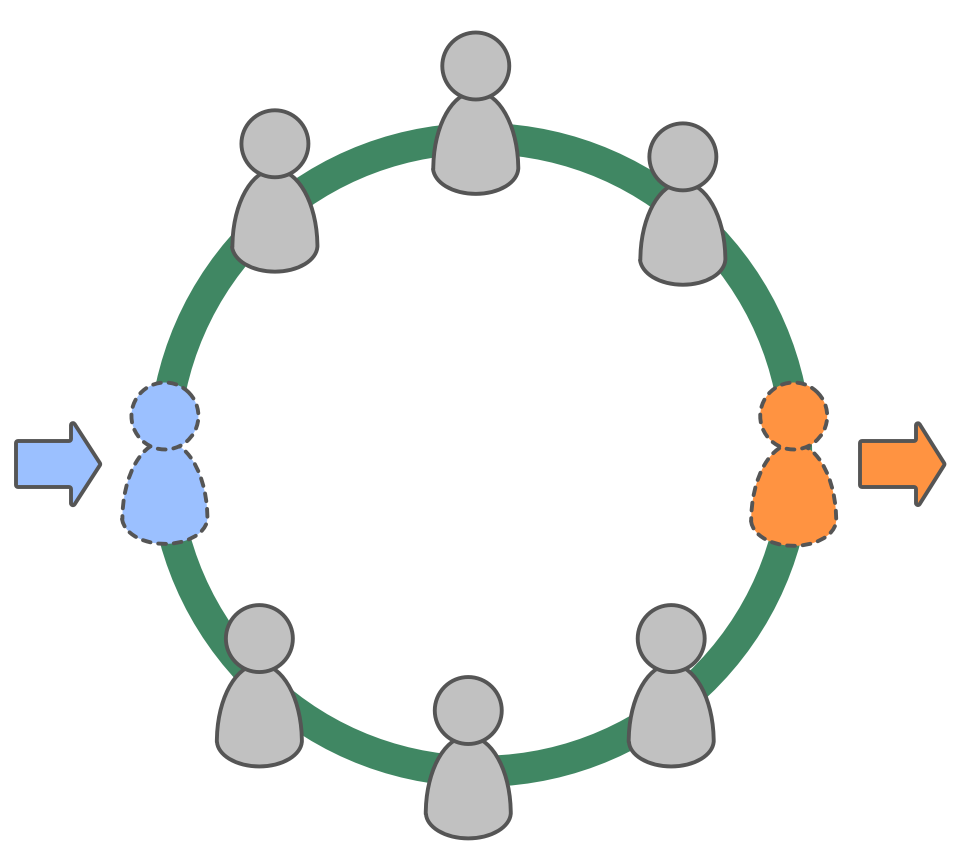
\includegraphics[keepaspectratio,width=\textwidth,height=0.75\textheight]{img/circle/enter-leave-circle.png}
\end{figure}

\begin{itemize}
\item define the process for entering the organization

\item define default role for a new member

\item define the process for leaving an organization

\end{itemize}

\section{Linking}
\label{linking}

\subsection{Connecting two circles}
\label{connectingtwocircles}

\begin{figure}[htbp]
\centering
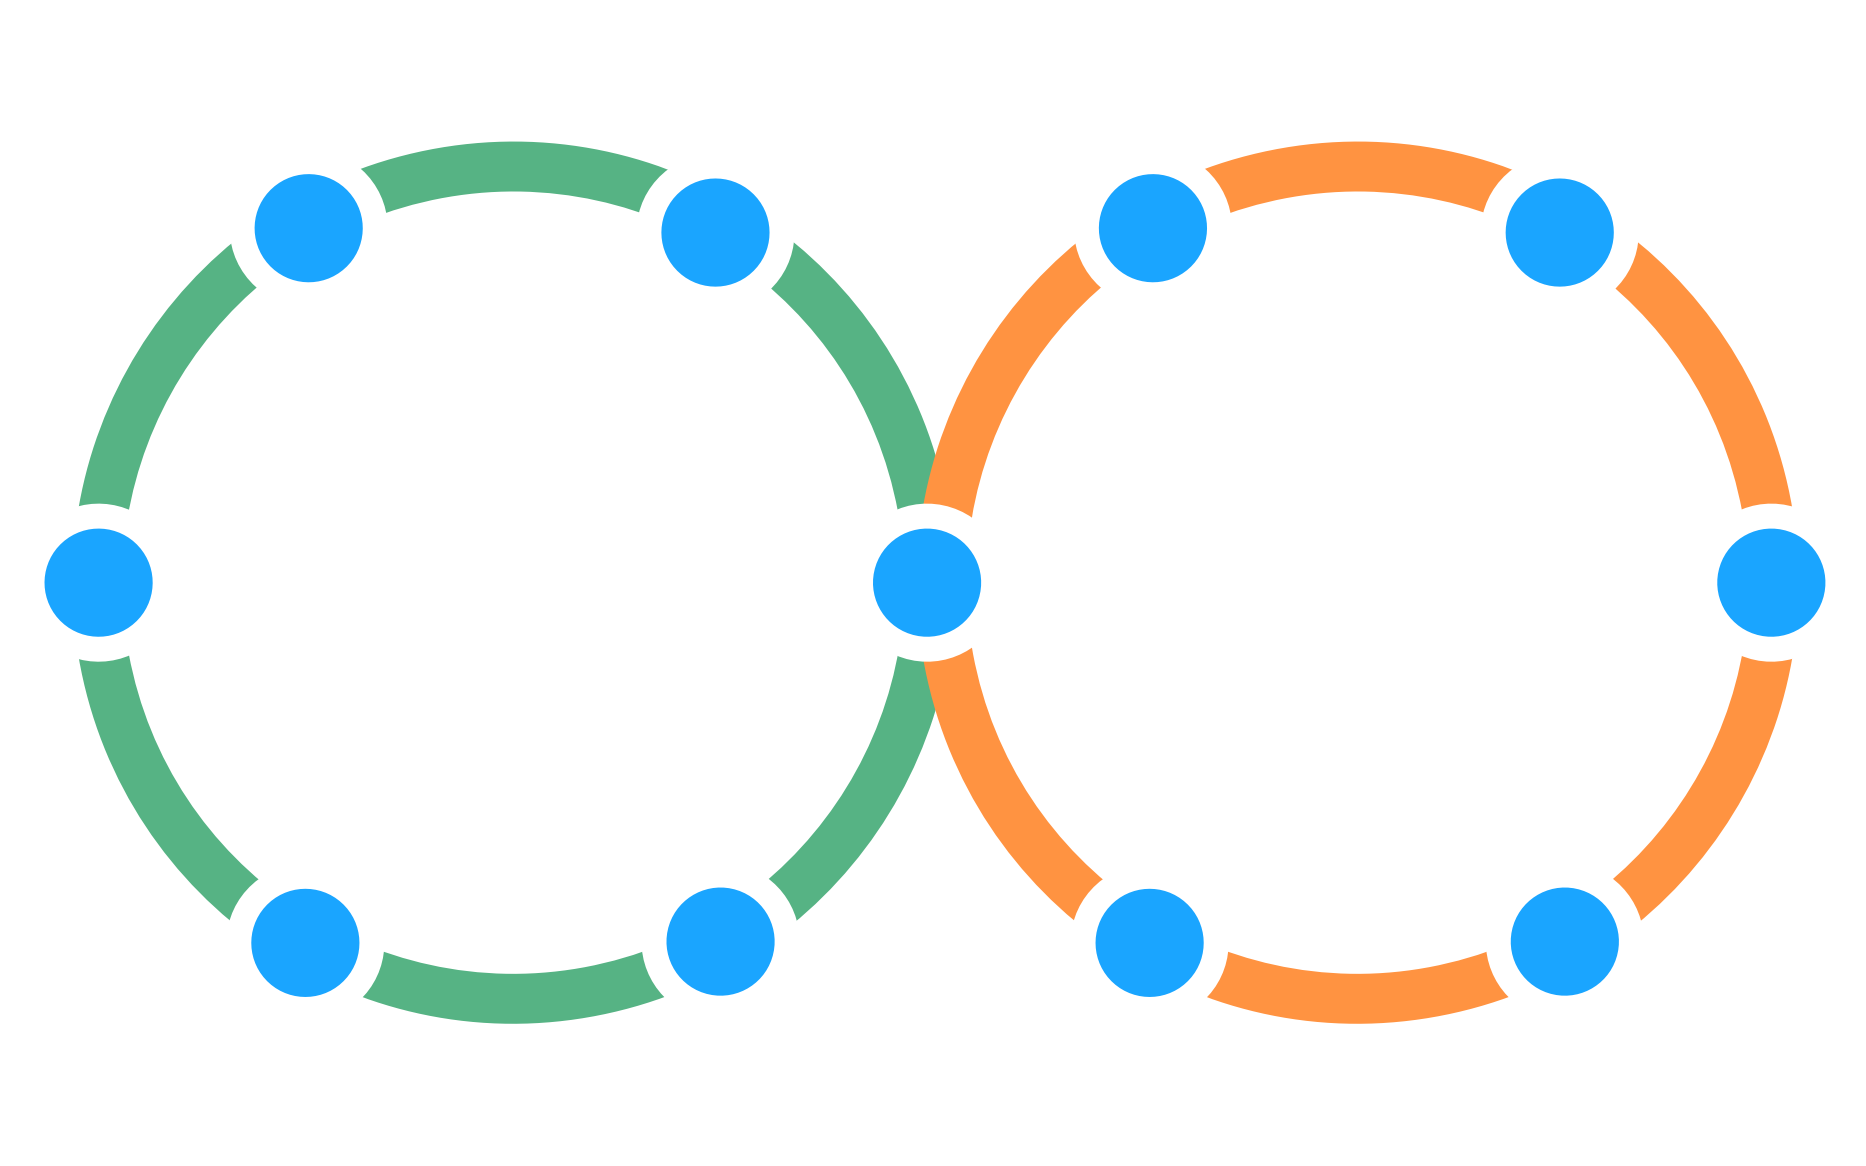
\includegraphics[keepaspectratio,width=\textwidth,height=0.75\textheight]{img/structural-patterns/link.png}
\end{figure}

\section{Transparent Salary}
\label{transparentsalary}

\begin{itemize}
\item transparent salaries need to be fair

\item perception of fairness is specific to organization

\item consider members and relevant stakeholders (e.g. investors)

\item classic sociocracy: everyone feels gains and losses

\item consider remuneration for changing roles

\item create strategy for transitioning towards new contracts and compensation agreements

\end{itemize}

\begin{figure}[htbp]
\centering
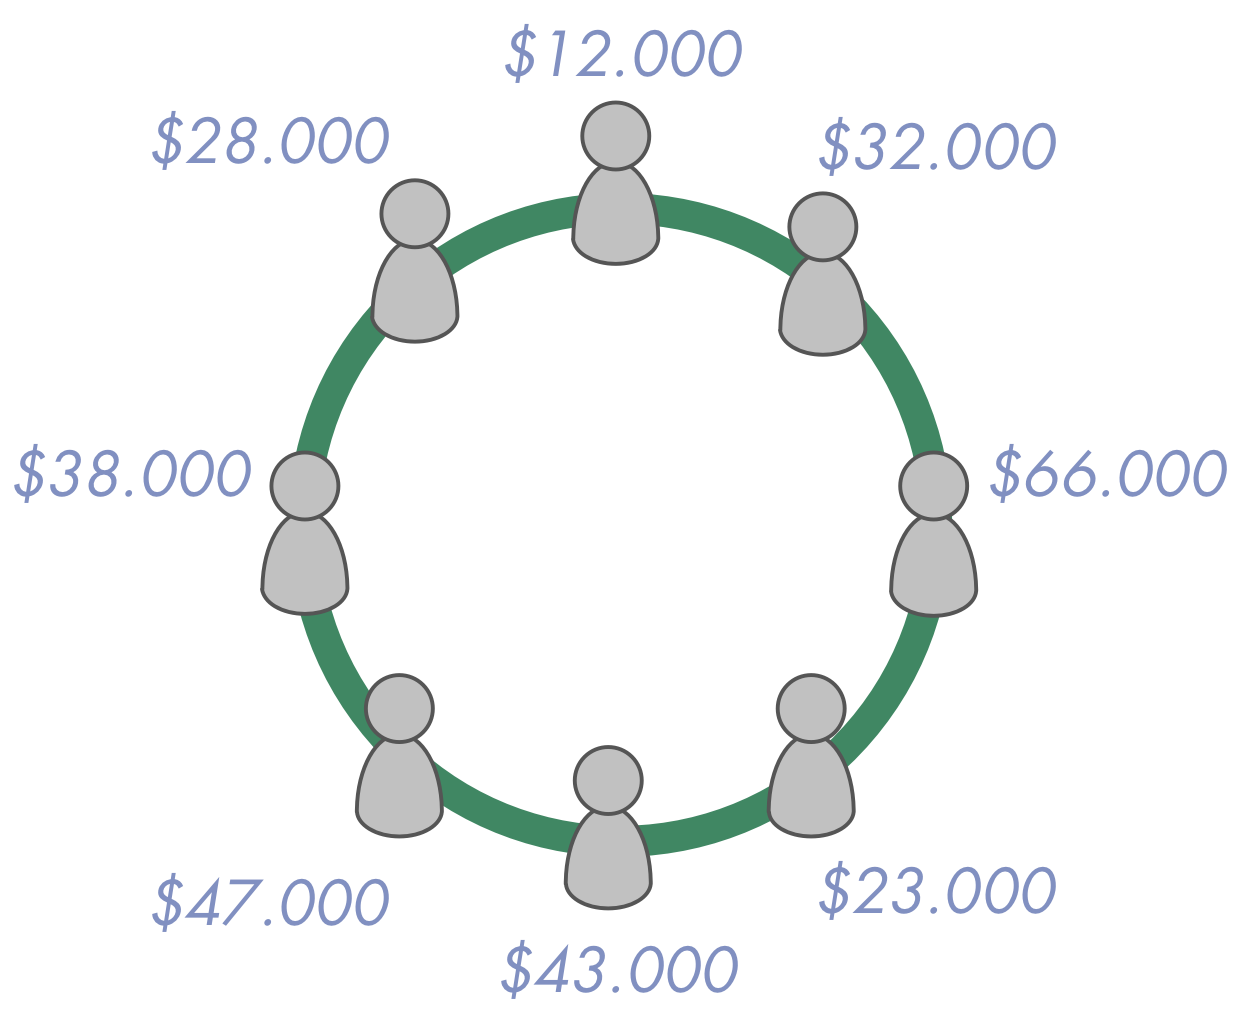
\includegraphics[keepaspectratio,width=\textwidth,height=0.75\textheight]{img/circle/transparent-salary.png}
\end{figure}

\part{Appendix}
\label{appendix}

\chapter{Changelog}
\label{changelog}

\textbf{2016--2--29}

\begin{itemize}
\item cleaned up image folder

\end{itemize}

\textbf{2016--01--28}

\begin{itemize}
\item Conversion of the material contained in the ``Introduction to Sociocracy 3.0'' slide deck

\end{itemize}

\textbf{2016--01--27}

\begin{itemize}
\item Initial setup of the patterns repository.

\end{itemize}
